\documentclass[12pt]{article}
\linespread{1}

% margins
\setlength{\textwidth}{6.5in}
\setlength{\textheight}{8.75in}
\setlength{\oddsidemargin}{-0.1in}
\setlength{\topmargin}{-0.1in}
\setlength{\baselineskip}{10pt}

% load packages
\usepackage{amsmath}
\usepackage{amsfonts}
\usepackage{lscape}
\usepackage[round]{natbib}
\usepackage{graphicx}
\graphicspath{{figures_old/}{figures/}{figures_old/roc}{figures_old/calibration_curves}}
\usepackage{amssymb}
\usepackage{color}
\usepackage{hyperref}
\usepackage{booktabs}
\usepackage{verbatim}
\usepackage{listings}

% style setup
\bibliographystyle{plainnat}
\pagestyle{empty}
\setlength\parindent{0pt}
\setlength{\parskip}{\baselineskip}

% new commands
\newcommand{\indist}{\overset{d}{\rightarrow}}
\newcommand{\inprob}{\overset{P}{\rightarrow}}
\newcommand{\tabby}{\hspace{10pt}}
\newcommand{\ones}{{\bf 1}}
\newcommand{\tp}{\intercal}
\newcommand{\iprod}[2]{\langle #1 , #2 \rangle}

\newcommand{\note}[1]{\textcolor{red}{#1}}

% header
\title{HOSEA project updates}
\author{Peter MacDonald}
\date{\today}

\begin{document}

%\maketitle

\subsubsection*{04/13 update}

\begin{itemize}
  \item Preliminary results on a small, {\bf balanced} subsample (5000 cases, 5000 controls).
  \item Training set of 9000 IDs, test set of 1000 IDs.
  \item Imputed missing variables with median.
  \item Lab data (blood tests, FOBT) and colonoscopies converted to longitudinal summaries (mean,max,min,...).
  \item Lab data restricted to time interval from `indexdate - 3 years' to `indexdate - 1 year'.
  \item No ICD code information, no medication information, no smoking status records (smoking status at index is in demographic variables).
  \item Logistic regression.
\end{itemize}

\begin{center}
\begin{table}[h!!]
\begin{tabular}{|l|l|l|}
\hline
\textbf{Predictors ($p=$ \# of predictors)}                                                & \textbf{Training AUC} & \textbf{Test AUC} \\ \hline
Demographic ($p=10$)                                     & 0.814                 & 0.818             \\ \hline
Charlson ($p=18$)                                     & 0.705               & 0.693         \\ \hline
Demographic + Charlson ($p=28$)             & 0.863                 & 0.862             \\ \hline
Labs ($p=210$)                                                 & 0.824                 & 0.824             \\ \hline
Demographic + Charlson + Labs ($p=238$) & 0.913                 & 0.910             \\ \hline
\end{tabular}
\end{table}
\end{center}

\pagebreak

\subsubsection*{04/20 update}

\begin{itemize}
  \item Preliminary results on a small, {\bf balanced} subsample (5000 cases, 5000 controls).
  \item Training set of 9000 IDs, test set of 1000 IDs.
  \item Imputed missing variables with median.
  \item {\bf Sets of predictors:}
  \begin{itemize}
    \item Demographic data includes race, age, weight, etc. ({\bf Demographic}).
    \item Charlson score inputs plus GERD diagnosis ({\bf Charlson}).
    \item Lab data (blood tests, FOBT) and colonoscopy data converted to longitudinal summaries (mean,max,min,...) ({\bf Labs}).
    \item Medication (H2R and PPI) converted to longitudinal summaries (mean,max,...) ({\bf Meds}).
  \end{itemize}
  \item Lab and medication data restricted to time interval from `indexdate - 3 years' to `indexdate - 1 year'.
  \item Logistic regression.
\end{itemize}

\begin{center}
\begin{table}[h!!]
\begin{tabular}{|l|l|l|}
\hline
\textbf{Predictors ($p=$ \# of predictors)}                                                & \textbf{Training AUC} & \textbf{Test AUC} \\ \hline
Demographic ($p=10$)                                     & 0.814                 & 0.818             \\ \hline
Charlson ($p=18$) & 0.705 & 0.693                                                            \\ \hline
Meds ($p=10$)                                                 & 0.604              & 0.598       \\ \hline
Demographic + Charlson + Labs + Meds ($p=240$)                                                 & 0.915                & 0.912            \\ \hline
\end{tabular}
\end{table}
\end{center}

\pagebreak

\subsubsection*{04/27 update}

\begin{itemize}
  \item Baseline logistic regression on entire sample (no blood labs, no medication data).
  \item Full sample contains $n = 6,649,108$ observations, with $n_{\text{control}} = 6,637,713$ and \\ $n_{\text{case}} = 11,395$.
  %\item About 582 controls for every case.
  \item Imputed numeric variables with medians, imputed smoking status at random, proportional to non-missing in sample (45\% current, 41\% former, 14\% never).
\end{itemize}

\begin{center}
\begin{tabular}{|l|l|l|}
\hline
\textbf{Predictors ($p=$ \# of predictors)}                                                & \textbf{Training AUC} & \textbf{Test AUC} \\ \hline
Demographic ($p=10$)                                     & 0.670                & 0.675            \\ \hline
Charlson ($p=18$) & 0.684 & 0.705                                                          \\ \hline
Demographic + Charlson ($p=28$)                                                 & 0.760               & 0.770     \\ \hline
\end{tabular}
\end{center}
{\bf Smoking status missingness.}

In the entire sample:
\begin{center}
\begin{tabular}{|l|l|l|l|l|}
\hline
\textbf{Smoking Status} & Current & Former & Never & Missing \\ \hline
Count & 1696052 & 1521806 & 537727 & 2893523 \\ \hline
Probability & 0.26 & 0.23 & 0.08 & \note{0.44} \\ \hline
\end{tabular}
\end{center}

Among cases:
\begin{center}
\begin{tabular}{|l|l|l|l|l|}
\hline
\textbf{Smoking Status} & Current & Former & Never & Missing \\ \hline
Count & 3901 & 3546 & 594 & 3354 \\ \hline
Probability & 0.34 & 0.31 & 0.05 & \note{0.29} \\ \hline
\end{tabular}
\end{center}

Among controls:
\begin{center}
\begin{tabular}{|l|l|l|l|l|}
\hline
\textbf{Smoking Status} & Current & Former & Never & Missing \\ \hline
Count & 1692151 & 1518260 & 537133 & 2890169 \\ \hline
Probability & 0.25 & 0.23 & 0.08 & \note{0.44} \\ \hline
\end{tabular}
\end{center}

\pagebreak

\subsubsection*{05/04 update}
\begin{itemize}
  \item Preliminary results on a balanced {\bf random sample} of 5000 cases and 5000 controls.
  \item Most missing variables imputed with their median, SmokeStatus imputed at random proportional to non-missing. %(about 45/41/14\% current/former/never)
  \item Training on 9000 observations, testing on 1000 observations.
  \item Baseline logistic regression fit with subsets of predictors, and all predictors.
  \item Random forest fit with all predictors.
\end{itemize}
\begin{center}
\begin{tabular}{|l|l|l|}
\hline
\textbf{Model/predictors ($p=$ \# of predictors)} & \textbf{Training AUC} & \textbf{Test AUC} \\ \hline
{\bf Logistic regression} & - & - \\ \hline
Demographic ($p=10$) & 0.669 & 0.676 \\ \hline
Charlson ($p=18$) & 0.689 & 0.659 \\ \hline
Meds ($p=10$) & 0.515 & 0.513 \\ \hline
Colonoscopies ($p=2$) & 0.513 & 0.502 \\ \hline
Labs ($p=200$) & 0.671 & 0.621 \\ \hline
All ($p=240$) & {\bf 0.814} & {\bf 0.778} \\ \hline
{\bf Random forest} & - & - \\ \hline
All ($p=240$) & {\bf 0.985} & {\bf 0.844} \\ \hline
\end{tabular}
\end{center}
{\bf Random forest variable importance.}
Most important blood lab measurements (all means of measurements over the 2 year window):
\begin{enumerate}
  \item Hematocrit value (CBC labs)
  \item MCH value (CBC labs)
  \item ALT value (LFT labs)
  \item Alk. Phos. value (LFT labs)
  \item AST value (LFT labs)
  \item White blood cells (WBC) value (CBC labs)
  \item Glucose value (BMP labs)
\end{enumerate}
{\bf Next steps:}
\begin{itemize}
  \item Better approaches to impute missing variables (esp. SmokeStatus).
  \item Improved non-linear classifiers for subsample.
  \item Logistic regression baselines for the full sample of 6M observations.
\end{itemize}

\pagebreak

\subsubsection*{05/11 update}
\begin{itemize}
  \item Baseline logistic regression on full sample (no medication data).
  \item $n = 6,649,108$ observations, with $n_{\text{control}} = 6,637,713$ and $n_{\text{case}} = 11,395$.
  %\item About 582 controls for every case.
  \item Most missing variables imputed with their median, SmokeStatus imputed at random proportional to non-missing.
  \item For lab information, only means of each measurement, no longitudinal information so far.
  \item \note{05/27 update:} Charlson and Demographic+Charlson updated to exclude Cancer and Metastatic Carcinoma.
\end{itemize}
\begin{center}
\begin{tabular}{|l|l|l|}
\hline
\textbf{Model/predictors ($p=$ \# of predictors)} & \textbf{Training AUC} & \textbf{Test AUC} \\ \hline
Demographic ($p=10$) & 0.670 & 0.675 \\ \hline
Charlson (\note{$p=16$}) & \note{0.684} & \note{0.705} \\ \hline
Demographic + Charlson (\note{$p=26$})                                                 & \note{0.760}               & \note{0.770}     \\ \hline
Colonoscopies ($p=2$) & 0.511 & 0.504 \\ \hline
Labs ($p=34$) & 0.604 & 0.601 \\ \hline
\note{Meds ($p=10$)} & \note{0.523} & \note{0.512} \\ \hline
%All ($p=64$) & {\bf 0.814} & {\bf 0.778} \\ \hline
\end{tabular}
\end{center}
{\bf Next steps:}
\begin{itemize}
  \item Process medication data.
  \item Approaches to impute missing variables (esp. SmokeStatus).
  \item Non-linear classifiers for subsample, plots/graphics to interpret predictor effects.
\end{itemize}

\pagebreak

\subsubsection*{05/18 update}

\begin{itemize}
  \item Medication data processed for full sample, new line (\note{red}) added to last week's table of baseline logistic regression AUCs.
  \item Gradient boosting implemented for the random sample of 5000 cases and 5000 controls.
\end{itemize}
\begin{center}
\begin{tabular}{|l|l|l|}
\hline
\textbf{Model/predictors ($p=$ \# of predictors)} & \textbf{Training AUC} & \textbf{Test AUC} \\ \hline
{\bf Logistic regression} & - & - \\ \hline
All ($p=240$) & 0.814 & 0.778 \\ \hline
{\bf Random forest} & - & - \\ \hline
All ($p=240$) & {\bf 0.985} & 0.844 \\ \hline
{\bf Gradient boosting} & - & - \\ \hline
All ($p=240$), no interactions & 0.900 & 0.847 \\ \hline
All ($p=240$), 2-way interactions & 0.924 & 0.857 \\ \hline
All ($p=240$), 3-way interactions & 0.937 & {\bf 0.864} \\ \hline
\end{tabular}
\end{center}
Same gradient boosting results without Charlson score inputs or GERD at index:
\begin{center}
\begin{tabular}{|l|l|l|}
\hline
\textbf{Model/predictors ($p=$ \# of predictors)} & \textbf{Training AUC} & \textbf{Test AUC} \\ \hline
{\bf Gradient boosting} & - & - \\ \hline
No Charlson inputs ($p=222$), no interactions & 0.881 & 0.811 \\ \hline
No Charlson inputs ($p=222$), 2-way interactions & 0.898 & 0.820 \\ \hline
No Charlson inputs ($p=222$), 3-way interactions & 0.909 & 0.817 \\ \hline
\end{tabular}
\end{center}

{\bf Next steps}
\begin{itemize}
  \item Scaling up gradient boosting, dealing with unbalanced classes in full sample.
  \item Plots/graphics to interpret black box models.
\end{itemize}

\pagebreak

\subsubsection*{05/25 update}

\begin{itemize}
  \item Results now without Cancer and Metastatic Carcinoma inputs to Charlson score.
  \item Implemented scalable \texttt{xgboost} model, test AUC \textbf{0.860}.
\end{itemize}

\textbf{Partial dependence plots} (from xgboost model).
Demographic variables:
\begin{center}
\begin{tabular}{cc}
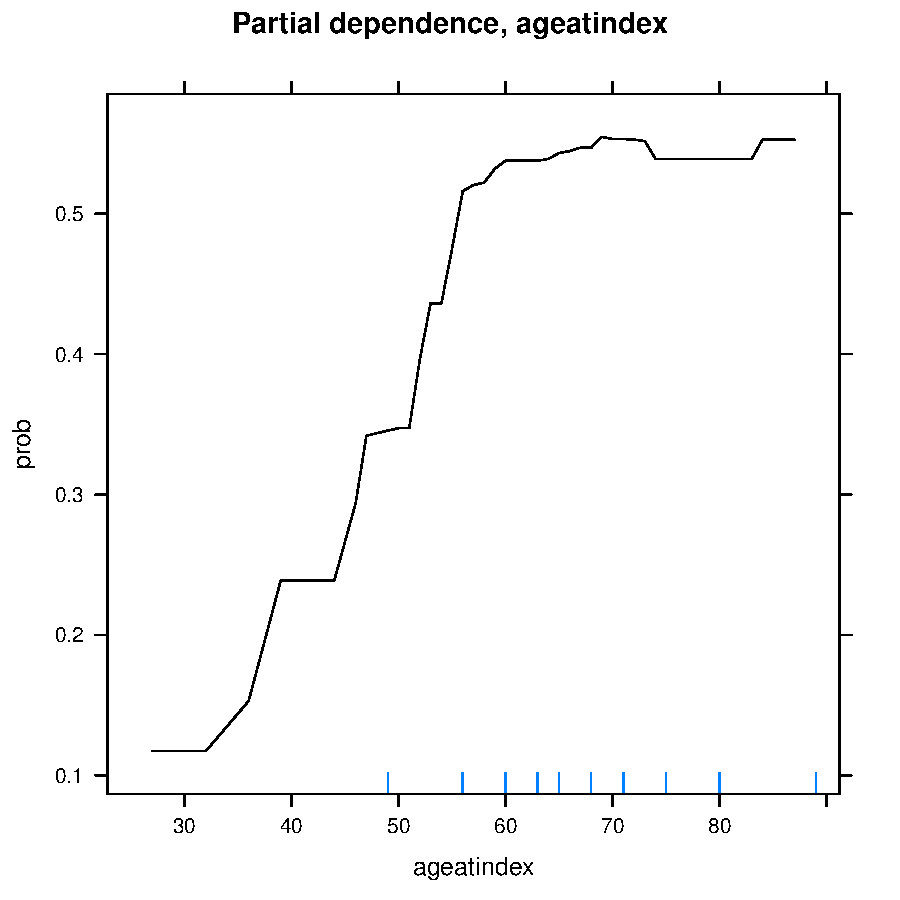
\includegraphics[width=.4\textwidth]{pdp_age.pdf} &
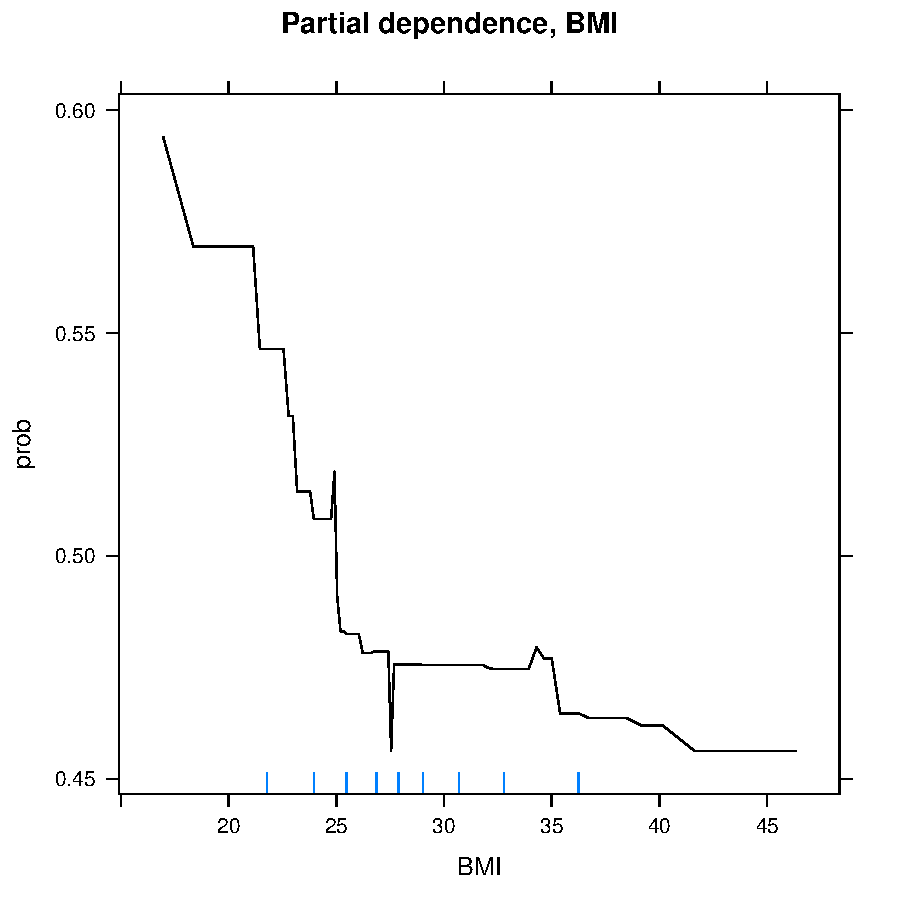
\includegraphics[width=.4\textwidth]{pdp_bmi.pdf} \\
\end{tabular}
\end{center}
Most influential blood lab variables:
\begin{center}
\begin{tabular}{cc}
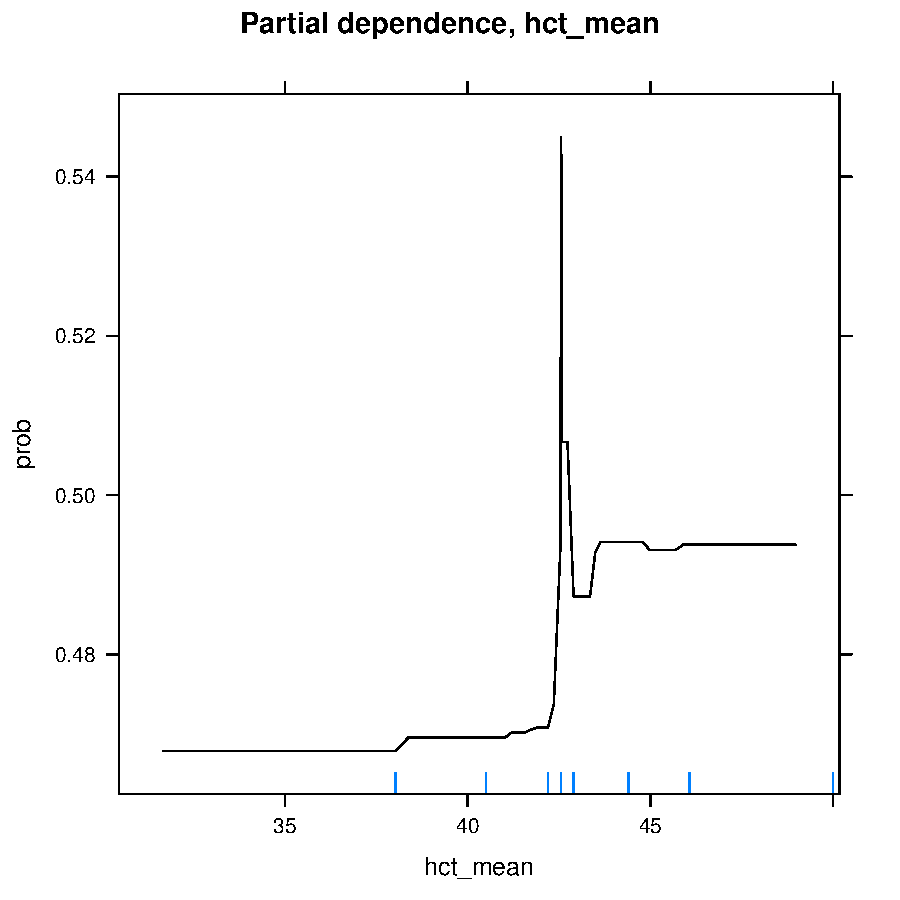
\includegraphics[width=.3\textwidth]{pdp_hct.pdf} &
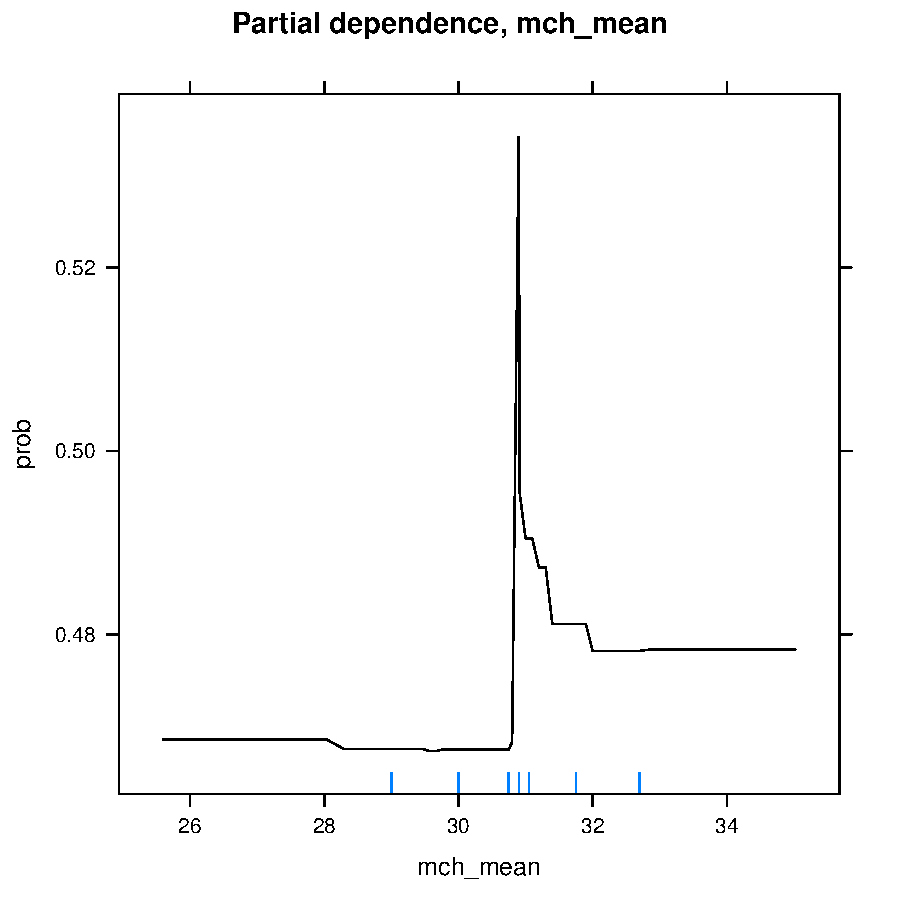
\includegraphics[width=.3\textwidth]{pdp_mch.pdf} \\
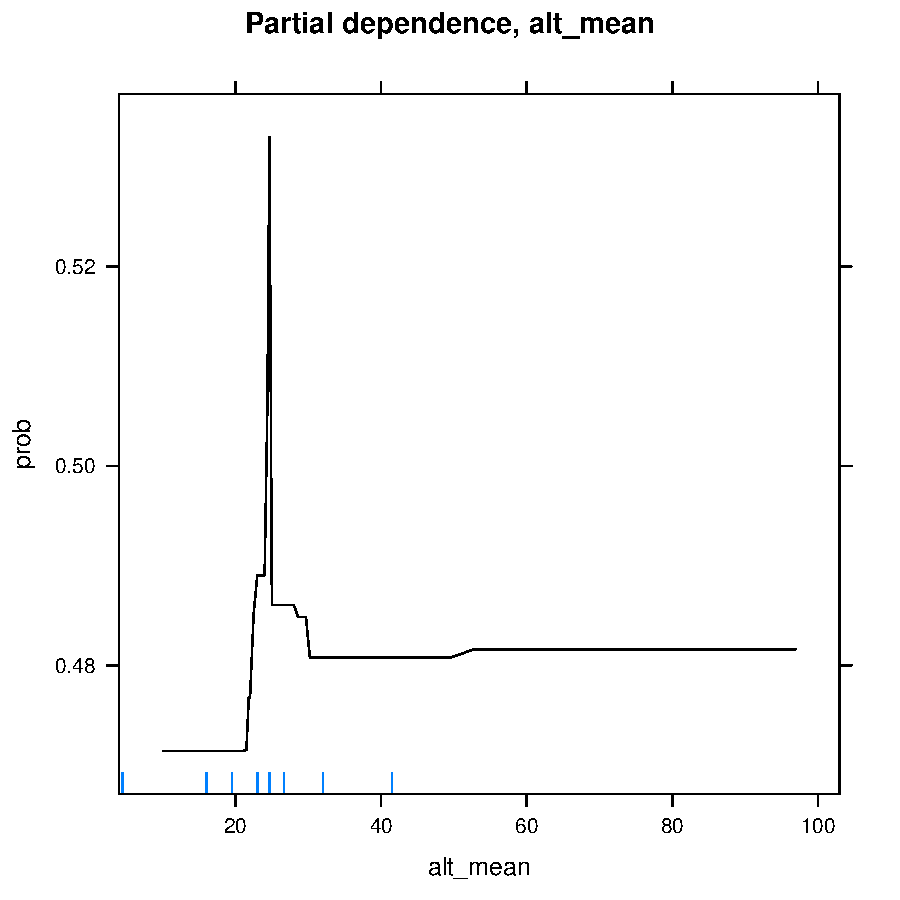
\includegraphics[width=.3\textwidth]{pdp_alt.pdf} &
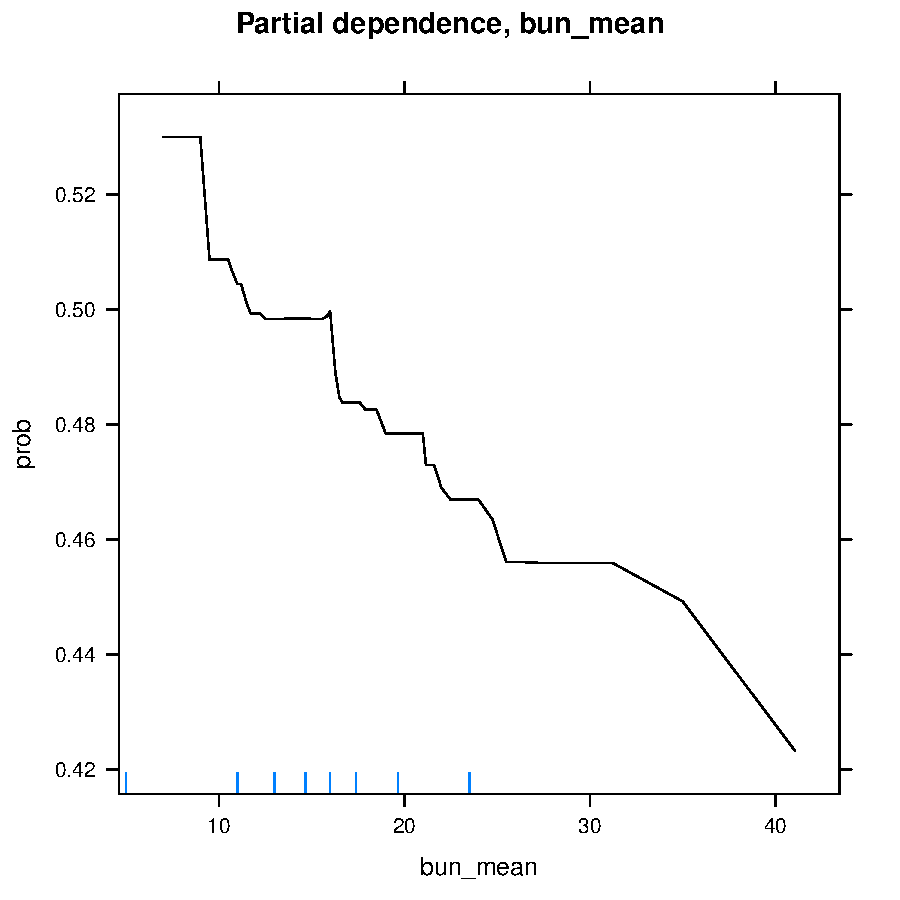
\includegraphics[width=.3\textwidth]{pdp_bun.pdf} \\
\end{tabular}
\end{center}

\textbf{Missingness rates for blood lab variables} (where `missing' means zero measurements of that variable in the 2 year window):
\begin{center}
\begin{tabular}{|l|l|l|}
\hline
\textbf{Proportion missing} & controls & cases \\ \hline
A1c\_mean (A1C Labs) & 0.51 & 0.52 \\ \hline
bun\_mean (BMP Labs) & 0.17 & 0.30 \\ \hline
hct\_mean (CBC Labs) & 0.20 & 0.50 \\ \hline
CRP\_mean (CRP Labs) & 0.95 & 0.94 \\ \hline
alkphos\_mean (LFT Labs) & 0.23 & 0.47 \\ \hline
chol\_mean (Lipid Labs) & 0.19 & 0.32 \\ \hline
\end{tabular}
\end{center}
\note{08/20: now with the new data, 4 year window from index-1 to index-5}
\begin{center}
\begin{tabular}{|l|l|l|}
\hline
\textbf{Proportion missing} & controls & cases \\ \hline
A1c\_mean (A1C Labs) & 0.43 & 0.47 \\ \hline
bun\_mean (BMP Labs) & 0.11 & 0.26 \\ \hline
hct\_mean (CBC Labs) & 0.12 & 0.46 \\ \hline
CRP\_mean (CRP Labs) & 0.93 & 0.91 \\ \hline
alkphos\_mean (LFT Labs) & 0.15 & 0.42 \\ \hline
chol\_mean (Lipid Labs) & 0.12 & 0.29 \\ \hline
\end{tabular}
\end{center}
\note{uniformly fewer missing, but rates are not cut in half, moreover heterogeneity of missingness between cases and controls is not fixed.}

\pagebreak

\subsubsection*{06/08 update}

\begin{itemize}
  \item Re-coded BMI/weight measurements?
  \item Re-run xgboost on balanced subsample with \texttt{NA}s, test AUC \textbf{0.880}, but it is using missing values to identify cases.
  \item Source of missingness? More detailed breakdown for LFT Labs.
\end{itemize}

\textbf{Updated partial dependence plots for blood lab variables.} Using new xgboost model on subsample.
\begin{center}
\begin{tabular}{cc}
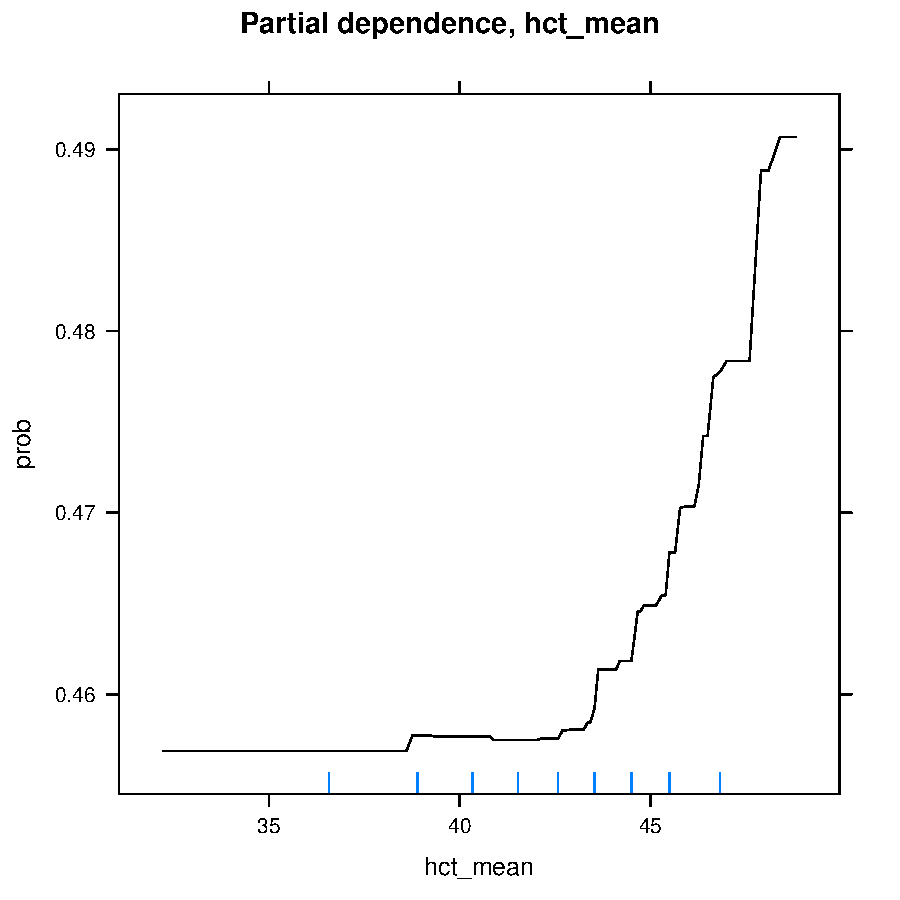
\includegraphics[width=.4\textwidth]{pdp_hct2.pdf} &
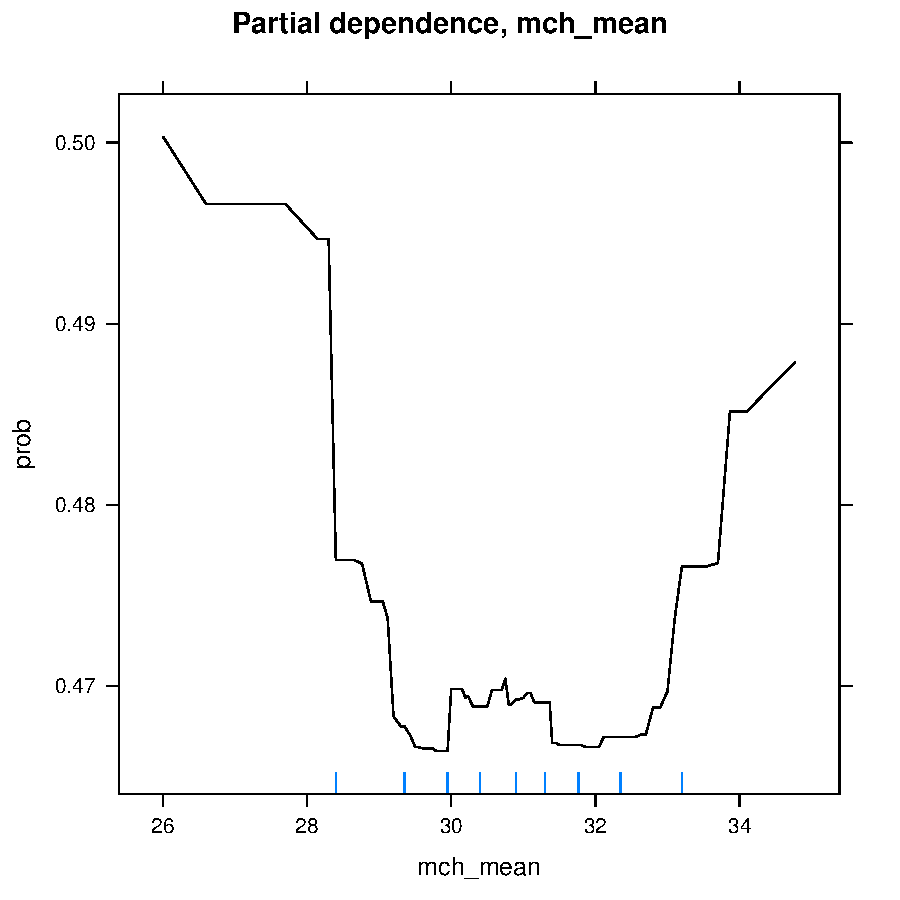
\includegraphics[width=.4\textwidth]{pdp_mch2.pdf} \\
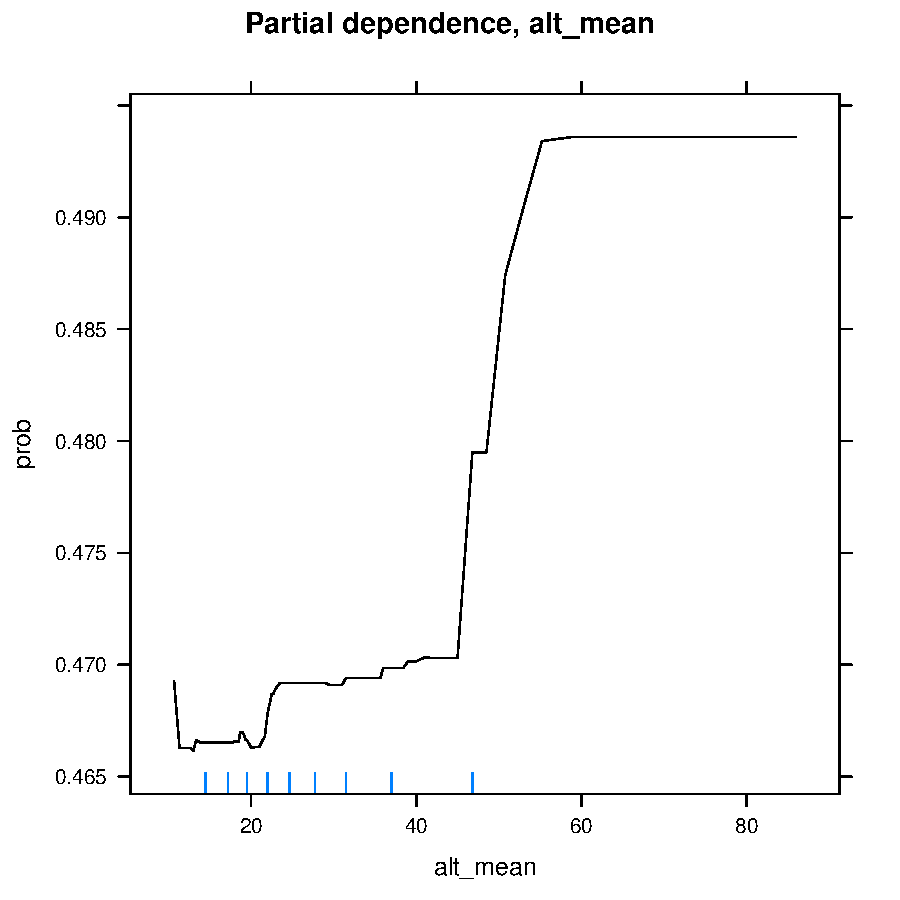
\includegraphics[width=.4\textwidth]{pdp_alt2.pdf} &
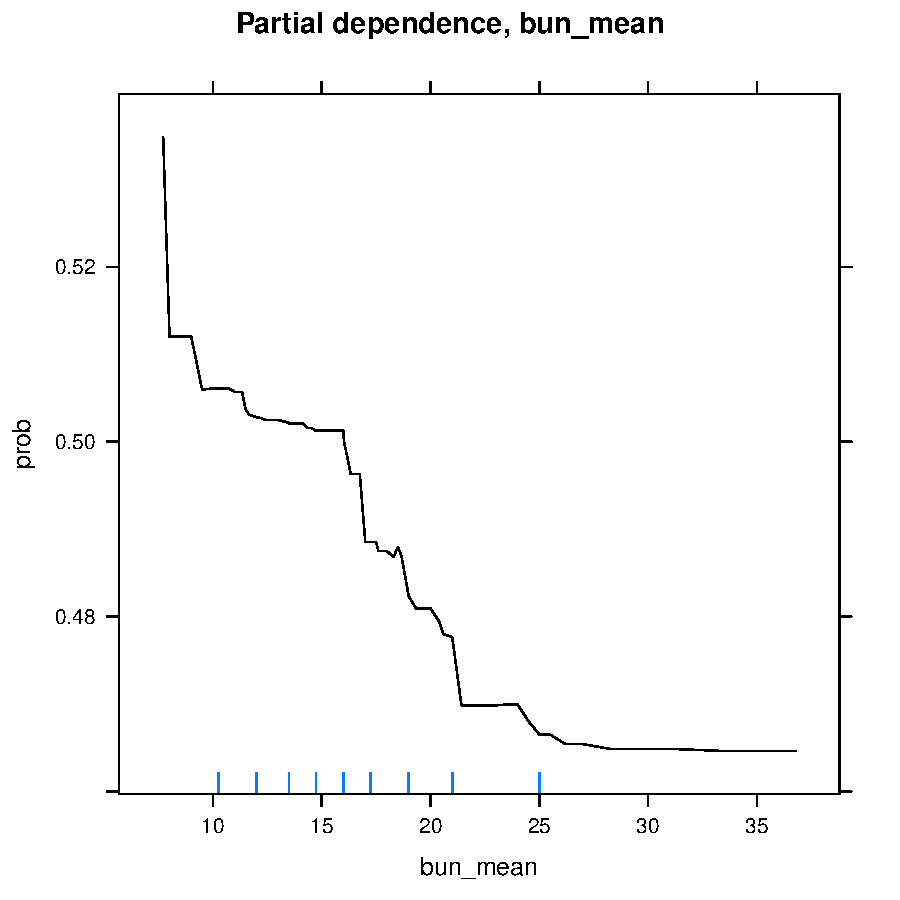
\includegraphics[width=.4\textwidth]{pdp_bun2.pdf} \\
\end{tabular}
\end{center}

\pagebreak

\textbf{Detailed breakdown of missingness for LFT labs.} (Prediction window is second and third years before index)
\begin{center}
\begin{tabular}{|l|l|l|}
\hline
\textbf{Mean \# of labs} & controls & cases \\ \hline
First year before index & 1.87 & 2.42 \\ \hline
Second year before index & 1.47 & 1.52 \\ \hline
Third year before index & 1.42 & 1.34 \\ \hline
\end{tabular}
\end{center}
Detailed breakdown for the prediction window (index minus 3 years to index minus 1 year):
\begin{center}
\begin{tabular}{|l|l|l|}
\hline
\textbf{Proportion} & controls & cases \\ \hline
At least 1 lab & 0.83 & 0.69 \\ \hline
At least 2 labs & 0.67 & 0.59 \\ \hline
At least 3 labs & 0.45 & 0.44 \\ \hline
At least 4 labs & 0.30 & 0.31 \\ \hline
At least 5 labs & 0.18 & 0.21 \\ \hline
\end{tabular}
\end{center}

\textbf{Next Steps:}
\begin{itemize}
  \item Imputation with xgboost
  \item Implement xgboost for entire sample
\end{itemize}

\pagebreak

\subsubsection*{06/22 update}

\begin{itemize}
  \item Set up code on GitLab (waljee-zhu-ml-projects/hosea-project).
  \item Received updated sample with recoded BMIs. BMIs are more likely to be missing for cases (14\%) than controls (8\%).
  \item Continuing to code imputation following Deng and Lumley (2021).
\end{itemize}

BMI comparison on the original sample data:
\begin{center}
\begin{tabular}{|l|l|l|l|l|l|l|}
\hline
 \textbf{Original BMI} & $< 20$ & $\in (20,25]$ & $\in (25,30]$ & $\in (30,35]$ & $\in (35,40]$ & $> 40$  \\ \hline
$\mathbb{P}(Control | BMI)$ & 0.9960 & 0.9978 & 0.9985 & 0.9985 & 0.9986 & 0.9986 \\ \hline
$\mathbb{P}(Case | BMI)$ & 0.0040 & 0.0022 & 0.0015 & 0.0015 & 0.0014 & 0.0014 \\ \hline
\end{tabular}
\end{center}

With the re-coded sample data:
\begin{center}
\begin{tabular}{|l|l|l|l|l|l|l|}
\hline
 \textbf{New BMI} & $< 20$ & $\in (20,25]$ & $\in (25,30]$ & $\in (30,35]$ & $\in (35,40]$ & $> 40$  \\ \hline
$\mathbb{P}(Control | BMI)$ & 0.9983 & 0.9985 & 0.9985 & 0.9984 & 0.9981 & 0.9979 \\ \hline
$\mathbb{P}(Case | BMI)$ & 0.0017 & 0.0015 & 0.0015 & 0.0016 & 0.0019 & 0.0021 \\ \hline
\end{tabular}
\end{center}

\pagebreak

\subsubsection*{06/29 update}

\begin{itemize}
  \item Now using updated data (new BMIs, Charlson scores).
  %\item Can bring back CANCER and MET\_CAR as predictors after re-processing?
  %\item Logistic regression is ``cheating'' with median imputation, using highly different missingess rates for Charlson scores
  \item For subsample, comparison of baseline logistic regression and xgboost models for different imputation approaches:
  \begin{enumerate}
    \item \textbf{No imputation}: leave NAs in the data, learn a classification for subjects with missing data (only compatible with xgboost).
    \item \textbf{Median imputation}: impute all variables with median/most common class.
    \item \textbf{Regression imputation}: impute by (linear) regression of each predictor variable on the others (similar to MICE).
    \item \textbf{Random sample imputation}: impute each predictor by sampling at random from the non-missing entries.
  \end{enumerate}
\end{itemize}

AUC results for xgboost/logistic regression for different imputation approaches. Results still on balanced subsample.
\begin{center}
\begin{tabular}{|l|l|l|l|}
\hline
\textbf{Imputation method/model} & \textbf{Training AUC} & \textbf{Test AUC} & \note{\textbf{Test AUC (complete records)}} \\ \hline
{\bf No imputation} & - & - & - \\ \hline
xgboost & 0.977 & 0.942 & \note{0.643} \\ \hline
{\bf Median imputation} & - & - & - \\ \hline
logistic regression & 0.834 & 0.810 & \note{0.585} \\ \hline
xgboost & 0.970 & 0.857 & \note{0.623} \\ \hline
{\bf Regression imputation} & - & - & - \\ \hline
logistic regression & 0.805 & 0.760 & \note{0.557} \\ \hline
xgboost & 0.948 & 0.815 & \note{0.705} \\ \hline
{\bf Random sample imputation} & - & - & - \\ \hline
logistic regression & 0.724 & 0.689 & \note{0.724} \\ \hline
xgboost & 0.919 & 0.729 & \note{\textbf{0.745}} \\ \hline
\end{tabular}
\end{center}

Regression imputation still has `regression to mean' effect for imputed values, imputed values have smaller variance than the true values (with observation error). Maybe try a version that imputes a rank then resamples from observed values.

% \textbf{Example:} Peptic Ulcer Disease (PUD) indicator.
%
% Among non-missing cases, 6.2\% have PUD=1. Among non-missing controls, 2.7\% have PUD=1.
%
% About 85\% of cases are missing PUD indicator, while about 47\% of controls are missing PUD indicator.
%
% After median imputation (PUD=NA becomes PUD=0 for all missing entries), 0.9\% of cases have PUD=1, 1.4\% of controls have PUD=1.

\pagebreak

\subsubsection*{07/06 update}

\begin{itemize}
  \item Source of missingness in the data? About 85\% of cases missing Charlson score inputs (compared to about 47\% of controls).
  \item Missingness in test set/use case?
  \item Updated \note{(in red)} last weeks results with a test set of 1000 complete records (226 cases, 774 controls).
  \begin{itemize}
    \item Poor generalization to complete cases for no imputation, median imputation implies that those models are fitting to the missingness, patterns won't continue to hold with fully observed data.
    \item Regression imputation still has `regression to mean' effect for imputed values, imputed values have smaller variance than the observed values (observation error).
    \item Good generalization of random sample imputation implies that there is no bias introduced from training on data with missingness.
  \end{itemize}
  %\item Memory issues fitting xgboost on the full data, will need to do some kind of batch training to handle the entire data.
\end{itemize}

\pagebreak

\subsubsection*{07/13 update}

\begin{itemize}
  \item Should we evaluate the model on complete records or missing/imputed records?
  \item Recall: previous results with an additional test set of 1000 complete records (226 cases, 774 controls).
  \begin{itemize}
    \item New comparison for \textbf{multiple} random sample imputation: imputes by sampling from non-missing entries several times (reps) for each missing value, training on the multiple imputed records.
    %\item Poor generalization to complete cases for no imputation, median imputation implies that those models are fitting to the missingness, patterns won't continue to hold with fully observed data.
    %\item Good generalization of random sample imputation implies that there is no bias introduced from training on data with missingness.
  \end{itemize}
  \item Memory issues fitting xgboost on the full data, implementing ``batched'' training.
\end{itemize}

AUC's for xgboost/logistic regression for different imputation approaches. Results still on balanced subsample.
\begin{center}
\begin{tabular}{|l|l|l|l|}
\hline
\textbf{Imputation method/} & \textbf{Training AUC} & \textbf{Test AUC} & \textbf{Test AUC} \\
\textbf{prediction model}& & \textbf{(imputed records)} & \textbf{(complete records)} \\ \hline
{\bf No imputation} & - & - & - \\ \hline
xgboost & 0.977 & 0.942 & 0.643 \\ \hline
{\bf Median imputation} & - & - & - \\ \hline
logistic regression & 0.834 & 0.810 & 0.585 \\ \hline
xgboost & 0.970 & 0.857 & 0.623 \\ \hline
{\bf Regression imputation} & - & - & - \\ \hline
logistic regression & 0.805 & 0.760 & 0.557 \\ \hline
xgboost & 0.948 & 0.815 & 0.705 \\ \hline
{\bf Random sample imputation} & - & - & - \\ \hline
logistic regression & 0.724 & 0.689 & 0.724 \\ \hline
xgboost & 0.919 & 0.729 & 0.745 \\ \hline
{\bf Multiple rand. samp.} & - & - & - \\ \hline
xgboost, 10 reps & 0.909 & 0.742 & 0.781 \\ \hline
xgboost, 20 reps & 0.939 & 0.765 & 0.820 \\ \hline
xgboost, 30 reps & 0.948 & 0.768 & 0.781 \\ \hline
\end{tabular}
\end{center}

Final two columns suggest two different evaluation metrics, ensuring the model performs well on \textbf{both} (A) new patients with imputed data and (B) new patients with fully observed blood labs, etc.

\pagebreak

\subsubsection*{07/20 update}

\begin{itemize}
  \item Continuing to test/tune imputation approaches.
  \item Notes on decision curve analysis.
\end{itemize}

\begin{center}
\begin{tabular}{|l|l|l|l|}
\hline
\textbf{Imputation method/} & \textbf{Training AUC} & \textbf{Test AUC} & \textbf{Test AUC} \\
\textbf{prediction model}& & \textbf{(imputed records)} & \textbf{(complete records)} \\ \hline
{\bf Separate class} & - & - & - \\ \hline
xgboost & 0.977 & 0.942 & 0.643 \\ \hline
{\bf Median} & - & - & - \\ \hline
logistic regression & 0.834 & 0.810 & 0.585 \\ \hline
xgboost & 0.970 & 0.857 & 0.623 \\ \hline
{\bf Regression} & - & - & - \\ \hline
logistic regression & 0.805 & 0.760 & 0.557 \\ \hline
xgboost & 0.948 & 0.815 & 0.705 \\ \hline
{\bf Regression v2} & - & - & - \\ \hline
logistic regression & 0.769 & 0.706 & 0.564 \\ \hline
xgboost & 0.928 & 0.722 & 0.764 \\ \hline
% {\bf ``Hybrid'' reg + dist'n match} & - & - & - \\ \hline
% logistic regression & 0.759 & 0.704 & 0.657 \\ \hline
% xgboost & 0.902 & 0.742 & 0.757 \\ \hline
{\bf Random sample} & - & - & - \\ \hline
logistic regression & 0.724 & 0.689 & 0.724 \\ \hline
xgboost & 0.919 & 0.729 & 0.756 \\ \hline
{\bf Multiple rand. samp.} & - & - & - \\ \hline
xgboost, 10 imputes $\times$ 50 trees & 0.909 & 0.742 & 0.781 \\ \hline
xgboost, 20 imputes $\times$ 25 trees & 0.906 & 0.750 & 0.778 \\ \hline
xgboost, 30 imputes $\times$ 20 trees & 0.909 & 0.765 & 0.788 \\ \hline
xgboost, 100 imputes $\times$ 5 trees & 0.898 & 0.762 & 0.806 \\ \hline
\end{tabular}
\end{center}

%Compare regression + dist'n match to random sample (with xgboost) and note that there is no significant difference in performance, implying that under the constraint of matched distributions, there is little additional information learned by regression approach.

\pagebreak

\subsubsection*{07/27 update}

\begin{itemize}
  %\item Drafted quarterly report.
  \item Continuing to tweak regression imputation approaches.
  \item Comparing parameters/number of imputations needed for multiple sample imputation.
  \item Notes on decision curve analysis.
\end{itemize}

\textbf{Next steps:}
\begin{itemize}
  \item Re-process new data when available%; compare missingness rates, total number of complete cases, baseline prediction AUCs.
\end{itemize}

\begin{center}
\begin{tabular}{|l|l|l|l|}
\hline
\textbf{Imputation method/} & \textbf{Training AUC} & \textbf{Test AUC} & \textbf{Test AUC} \\
prediction model& & \textbf{(imputed records)} & \textbf{(complete records)} \\ \hline
{\bf Separate class} & - & - & - \\ \hline
xgboost & 0.977 & 0.942 & 0.643 \\ \hline
{\bf Median} & - & - & - \\ \hline
logistic regression & 0.834 & 0.810 & 0.585 \\ \hline
xgboost & 0.970 & 0.857 & 0.623 \\ \hline
{\bf Regression} & - & - & - \\ \hline
logistic regression & 0.759 & 0.704 & 0.657 \\ \hline
xgboost & 0.902 & 0.742 & 0.757 \\ \hline % This is the current best regression imputation approach (hybrid, distn matching, but without using lab means to impute other lab means)
{\bf Single rand. samp.} & - & - & - \\ \hline
logistic regression & 0.724 & 0.689 & 0.724 \\ \hline
xgboost & 0.919 & 0.729 & 0.756 \\ \hline
{\bf Multiple rand. samp.} & - & - & - \\ \hline
xgboost, 10 imputes & 0.909 & 0.742 & 0.781 \\ \hline
xgboost, 20 imputes & 0.906 & 0.750 & 0.778 \\ \hline
xgboost, 30 imputes & 0.909 & 0.765 & 0.788 \\ \hline
xgboost, 100 imputes & 0.898 & 0.762 & 0.806 \\ \hline % all with 500-600 total trees
\end{tabular}
\end{center}

\pagebreak

\subsubsection*{08/03 update}

\begin{itemize}
  \item Received new data, loading/processing files
  \item Still issues with missing Charlson scores (0's vs NAs), relationship between CaseControl indicator and number of visits.
\end{itemize}

\pagebreak

\subsubsection*{08/17 update}

\begin{itemize}
  \item Processed longitudinal summaries for BMP labs. Missingness rates down but still different for cases and controls. Continuing to process new blood lab data.
  \item Incidence rates for some example Charlson inputs: Peptic Ulcer Disease, Renal Disease, GERD. Full tables for all inputs are on the next page.
\end{itemize}


\begin{center}
\begin{tabular}{|l|l|l|}
  \hline
Variable {\bf (ignoring NA's)} & Among cases & Among controls \\ \hline
pud                     & 6.8\% (120/1762)            & 3.8\% (142821/3803451)               \\ \hline
RD                      & 11.8\% (208/1762)            & 12.1\% (460302/3803451)               \\ \hline
GERD                    & -             & - \\ \hline
\end{tabular}

\begin{tabular}{|l|l|l|}
  \hline
Variable {\bf (impute NA's as 0's)} & Among cases & Among controls \\ \hline
pud                     & 1.1\% (120/11395)            & 2.2\% (142821/6637713)               \\ \hline
RD                      & 1.8\% (208/11395)            & 6.9\% (460302/6637713)                \\ \hline
GERD                    & 17.9\% (2044/11395)            &  15.7\% (1039206/6637713) \\ \hline
\end{tabular}
\end{center}

Cross-classified by number of BMP lab results (0, 1 or 2+):

Peptic Ulcer Disease, {\bf controls}:
\begin{center}
\begin{tabular}{|l|l|l|l|}
  \hline
Number of BMP labs & 0 & 1 & NA \\ \hline
0                   & 29.3\% & 0.9\% & 69.8\% \\ \hline
1                     & 32.2\% & 0.9\% & 66.8\% \\ \hline
2+                    & 61.5\% & 2.5\% & 36.0\% \\ \hline
\end{tabular}
\end{center}

Peptic Ulcer Disease, {\bf cases}:
\begin{center}
\begin{tabular}{|l|l|l|l|}
  \hline
Number of BMP labs & 0 & 1 & NA \\ \hline
0                   & 8.6\% & 0.7\% & 90.8\% \\ \hline
1                     & 10.7\% & 0.4\% & 88.8\% \\ \hline
2+                    & 17.0\% & 1.3\% & 81.7\% \\ \hline
\end{tabular}
\end{center}

% GERD, {\bf controls}:
% \begin{center}
% \begin{tabular}{|l|l|l|}
%   \hline
% Number of BMP labs & 0 & 1 \\ \hline
% 0                   & 93.1\% & 6.9\% \\ \hline
% 1                     & 91.9\% & 8.1\% \\ \hline
% 2+                    & 82.2\% & 17.8\% \\ \hline
% \end{tabular}
% \end{center}
%
% GERD, {\bf cases}:
% \begin{center}
% \begin{tabular}{|l|l|l|}
%   \hline
% Number of BMP labs & 0 & 1 \\ \hline
% 0                   & 90.3\% & 9.7\% \\ \hline
% 1                     & 86.3\% & 13.7\% \\ \hline
% 2+                    & 78.5\% & 21.5\%  \\ \hline
% \end{tabular}
% \end{center}

\pagebreak

Full tables for all Charlson indicators (\note{red} indicates these variables have been dropped from past models):

\begin{center}
\begin{tabular}{|l|l|l|}
  \hline
Variable {\bf (ignoring NA's)} & Among cases & Among controls \\ \hline
\note{CANCER}                  & 30.5\% (538/1762)         & 18.3\% (695558/3803451)        \\ \hline
CHF                     & 12.3\% (217/1762)            & 11.8\% (450090/3803451)               \\ \hline
CTD                     & 2.9\% (51/1762)            & 3.0\% (115492/3803451)               \\ \hline
DEM                     & 1.4\% (24/1762)          & 2.3\% (85704/3803451)              \\ \hline
DIAB\_C                 & 15.5\% (273/1762)            &  13.8\% (525226/3803451)              \\ \hline
HIV                     & 0.3\% (6/1762)            & 0.8\% (30507/3803451)                \\ \hline
\note{MET\_CAR}                & 6.6\% (117/1762)            & 1.3\% (47696/3803451)               \\ \hline
MLD                     & 9.1\% (160/1762)            & 8.0\% (305462/3803451)               \\ \hline
MSLD                    & 0.7\% (13/1762)            & 0.8\% (29495/3803451)              \\ \hline
PARA                    & 1.9\% (33/1762)            & 1.9\% (72051/3803451)               \\ \hline
RD                      & 11.8\% (208/1762)            & 12.1\% (460302/3803451)               \\ \hline
cd                      & 16.3\% (287/1762)            & 15.3\% (582328/3803451)               \\ \hline
copd                    & 43.1\% (759/1762)             & 35.9\% (1365577/3803451)               \\ \hline
diab\_nc                & 44.6\% (786/1762)            & 44.8\% (1702629/3803451)               \\ \hline
mi                      & 9.1\% (161/1762)            & 7.0\% (264731/3803451)               \\ \hline
pud                     & 6.8\% (120/1762)            & 3.8\% (142821/3803451)               \\ \hline
pvd                     & 20.1\% (354/1762)             & 16.0\% (609425/3803451)               \\ \hline
GERD                    & -             & - \\ \hline
\end{tabular}

\begin{tabular}{|l|l|l|}
  \hline
Variable {\bf (impute NA's as 0's)} & Among cases & Among controls \\ \hline
\note{CANCER}                  & 4.7\% (538/11395)           &  10.5\% (69558/6637713)              \\ \hline
CHF                     & 1.9\% (217/11395)            & 6.8\% (450090/6637713)                \\ \hline
CTD                     & 0.4\% (51/11395)             & 1.7\% (115492/6637713)               \\ \hline
DEM                     & 0.2\% (24/11395)             & 1.3\% (85704/6637713)                \\ \hline
DIAB\_C                 & 2.4\% (273/11395)             & 7.9\% (525226/6637713)               \\ \hline
HIV                     & 0.1\% (6/11395)            & 0.5\% (30507/6637713)                \\ \hline
\note{MET\_CAR}                & 1.0\% (117/11395)             & 0.7\% (47696/6637713)              \\ \hline
MLD                     & 1.4\% (160/11395)            & 4.6\% (305462/6637713)                \\ \hline
MSLD                    & 0.1\% (13/11395)            & 0.4\% (29459/6637713)              \\ \hline
PARA                    & 0.3\% (33/11395)            & 1.1\% (72051/6637713)               \\ \hline
RD                      & 1.8\% (208/11395)            & 6.9\% (460302/6637713)                \\ \hline
cd                      & 2.5\% (287/11395)            & 8.8\% (582328/6637713)               \\ \hline
copd                    & 6.7\% (759/11395)            & 20.6\% (1365577/6637713)               \\ \hline
diab\_nc                & 6.9\% (786/11395)             & 25.6\% (1702629/6637713)               \\ \hline
mi                      & 1.4\% (161/11365)            & 4.0\% (264731/6637713)               \\ \hline
pud                     & 1.1\% (120/11395)            & 2.2\% (142821/6637713)               \\ \hline
pvd                     & 3.1\% (354/11395)            & 9.2\% (609425/6637713)               \\ \hline
GERD                    & 17.9\% (2044/11395)            &  15.7\% (1039206/6637713) \\ \hline
\end{tabular}
\end{center}

\pagebreak

\subsubsection*{08/31 update}

\begin{itemize}
  \item Re-fit xgboost models on new subsampled data (compare to 07/27 results). \\ $n_{\mathrm{train}}=9000$, $n_{\mathrm{test}}=1000$, $n_{\mathrm{complete.test}}=1000$.
  \item Compare (xgboost) model performance with different groups of variables included.
  \item Ongoing: a proxy for number of visits to better impute Charlson ICD codes?
\end{itemize}

Comparing different imputation approaches and prediction models:
\begin{center}
\begin{tabular}{|l|l|l|l|}
\hline
\textbf{Imputation method/} & \textbf{Training AUC} & \textbf{Test AUC} & \textbf{Test AUC} \\
prediction model& & \textbf{(imputed records)} & \textbf{(complete records)} \\ \hline
{\bf Separate class} & - & - & - \\ \hline
xgboost & 0.985 & 0.962 & 0.582 \\ \hline
{\bf Median} & - & - & - \\ \hline
logistic regression & 0.853 & 0.846 & 0.583 \\ \hline
xgboost & 0.963 & 0.911 & 0.618 \\ \hline
{\bf Regression} & - & - & - \\ \hline
logistic regression & 0.772 & 0.726 & 0.651 \\ \hline
xgboost & 0.911 & 0.750 & 0.798 \\ \hline % This is the current best regression imputation approach (hybrid, distn matching, without using lab means to impute other lab means)
{\bf Single rand. samp.} & - & - & - \\ \hline
logistic regression & 0.739 & 0.695 & 0.703 \\ \hline
xgboost & 0.916 & 0.780 & 0.833 \\ \hline
{\bf Multiple rand. samp.} & - & - & - \\ \hline
xgboost, 10 imputes & 0.942 & 0.824 & 0.885 \\ \hline
xgboost, 20 imputes & 0.935 & 0.820 & 0.872 \\ \hline
xgboost, 30 imputes & 0.943 & 0.810 & 0.879 \\ \hline
xgboost, 100 imputes & 0.931 & 0.824 & 0.891 \\ \hline % all with 500-600 total trees
\end{tabular}
\end{center}

Comparing different included variables (imputing with single random sampling, fit with xgboost):
\begin{center}
\begin{tabular}{|l|l|l|l|}
\hline
\textbf{Variables included} & \textbf{Training AUC} & \textbf{Test AUC} & \textbf{Test AUC} \\
 & & \textbf{(imputed records)} & \textbf{(complete records)} \\ \hline
Demographic ($p=11$) & 0.743 & 0.700 & 0.663 \\ \hline
Charlson + GERD ($p=16$) & 0.600 & 0.542 & 0.530 \\ \hline
Medications ($p=10$) & 0.594 & 0.501 & 0.539 \\ \hline
Labs ($p=202$) & 0.903 & 0.687 & 0.829 \\ \hline
\end{tabular}
\end{center}

%\bibliography{mybib}

\pagebreak

\subsubsection*{09/21 update}

{\bf Overall missingness of Charlson score inputs.} A histogram of the total number of visits in the 4-year prediction window:

\begin{center}
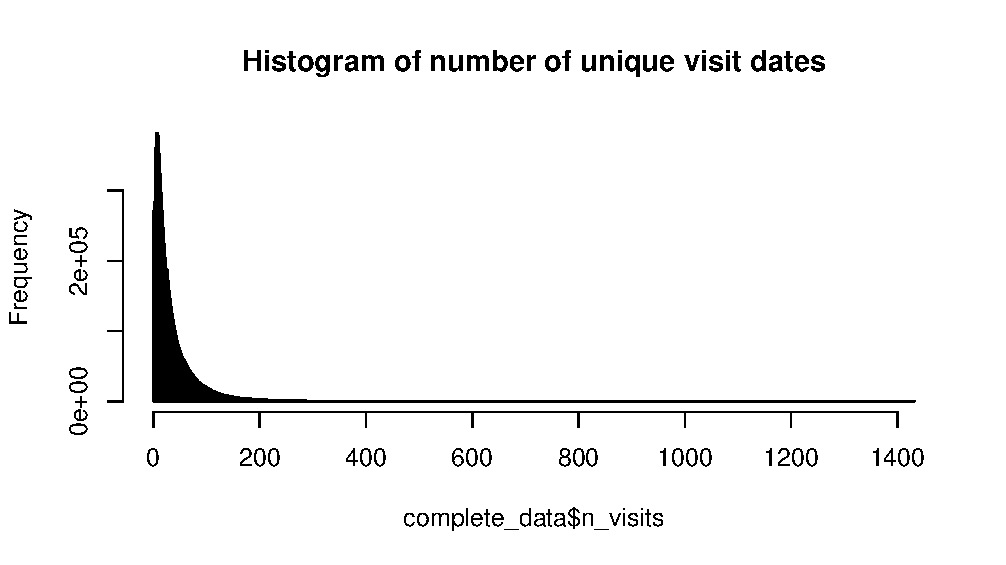
\includegraphics[width=.7\textwidth]{nvisits_hist.pdf}
\end{center}

The median control has 22 visits, while the median case has 33 visits.

Proportion of observed Charlson scores plotted against number of visits, separating controls (black) and cases (red):

\begin{center}
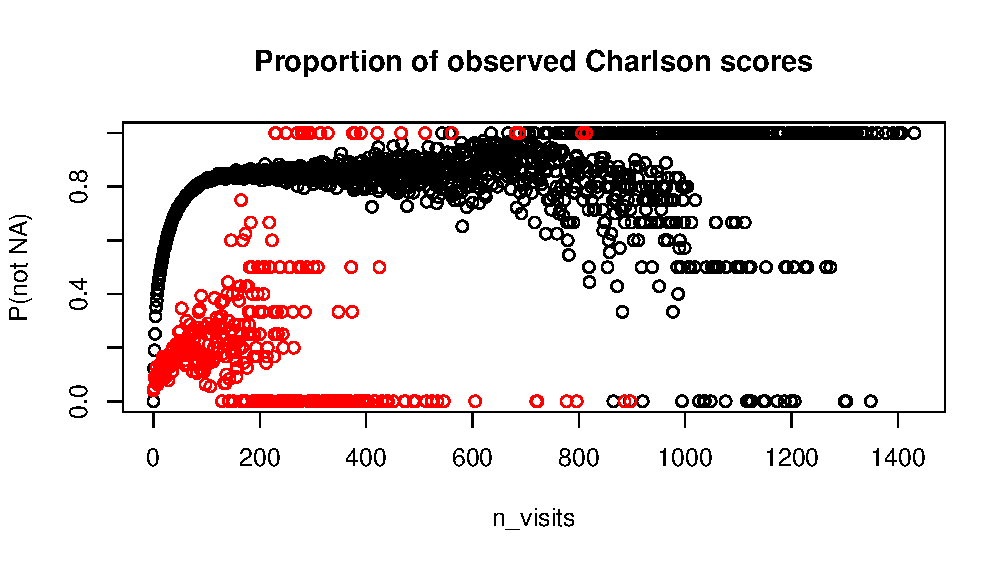
\includegraphics[width=.6\textwidth]{nvisits_scatter.pdf}
\end{center}

The same plot restricted to $\leq 200$ visits.
%Sample sizes are reasonably high (cases have a mean of 55 patients at each level of n\_visits):

\begin{center}
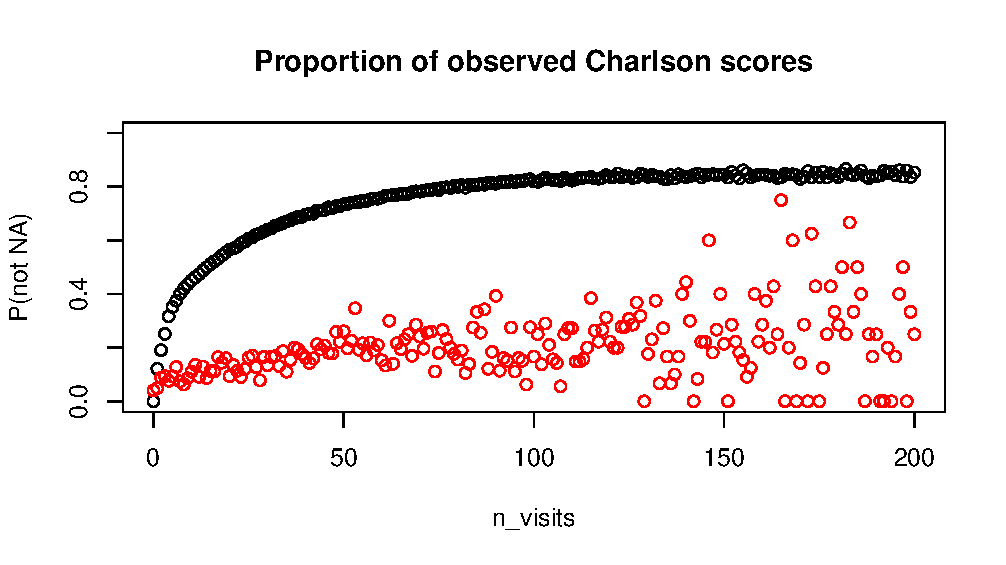
\includegraphics[width=.6\textwidth]{nvisits_scatter200.pdf}
\end{center}

{\bf Example: missingness of COPD.} Proportion of patients coded COPD=1, plotted against number of visits, separating controls (black) and cases (red):

\begin{center}
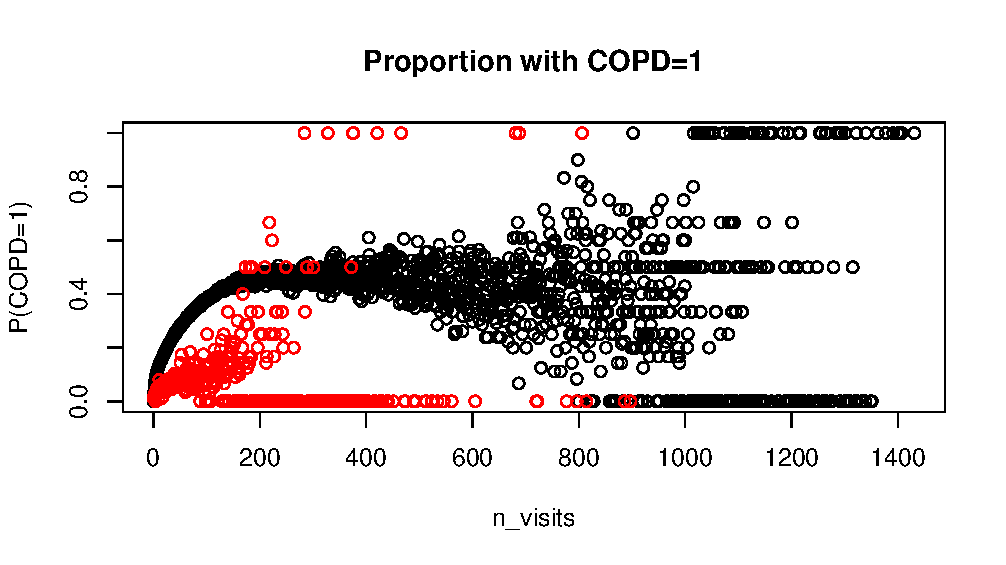
\includegraphics[width=.6\textwidth]{nvisits_scatterCOPD.pdf}
\end{center}

The same plot restricted to $\leq 200$ visits. The blue line is a model-based estimate of \\ $\mathbb{P}(\text{COPD}=1 | \text{n\_visits})$ using pooled case and control data.

\begin{center}
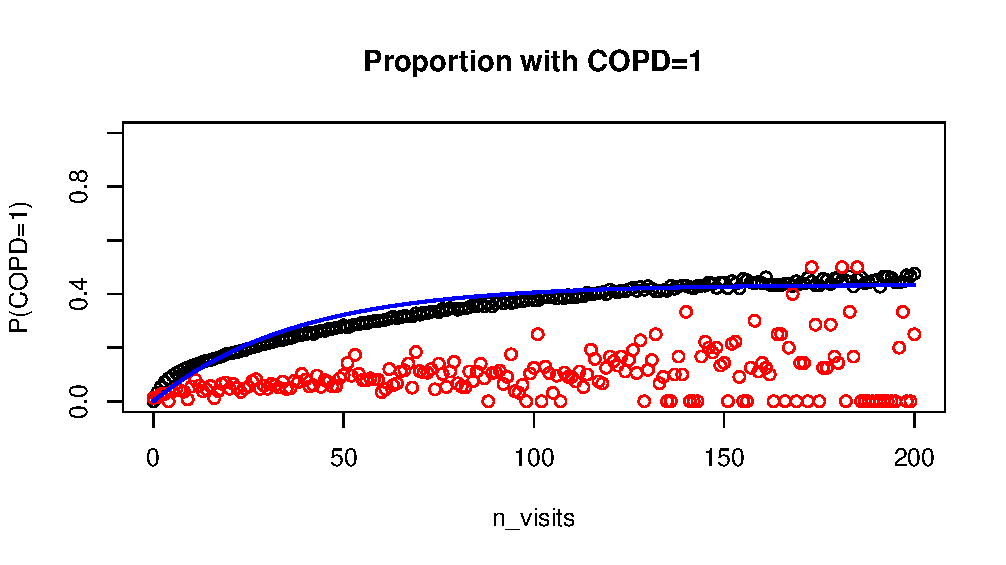
\includegraphics[width=.6\textwidth]{nvisits_scatterCOPD200.pdf}
\end{center}

For cases only, created a new COPD indicator based on the `alldxscx' table. For ICD9, 1 means you have a code `49x', for ICD10, 1 means you have a code starting with 'J44'.

Cross-classification of old and new indicator for total of 11,395 cases (overall proportions in parentheses).

\begin{center}
\begin{tabular}{|l|l|l|}
\hline
 & New COPD=1 & New COPD=0/NA \\ \hline
 Old COPD=1 & 7845 (0.688) & 2791 (0.245) \\ \hline
 New COPD=0/NA & 160 (0.014) & 599 (0.053) \\ \hline
\end{tabular}
\end{center}

Proportion of patients with COPD=1 plotted against number of visits, restricted to $\leq 200$ visits, with the old indicator in red and the new indicator in blue.

\begin{center}
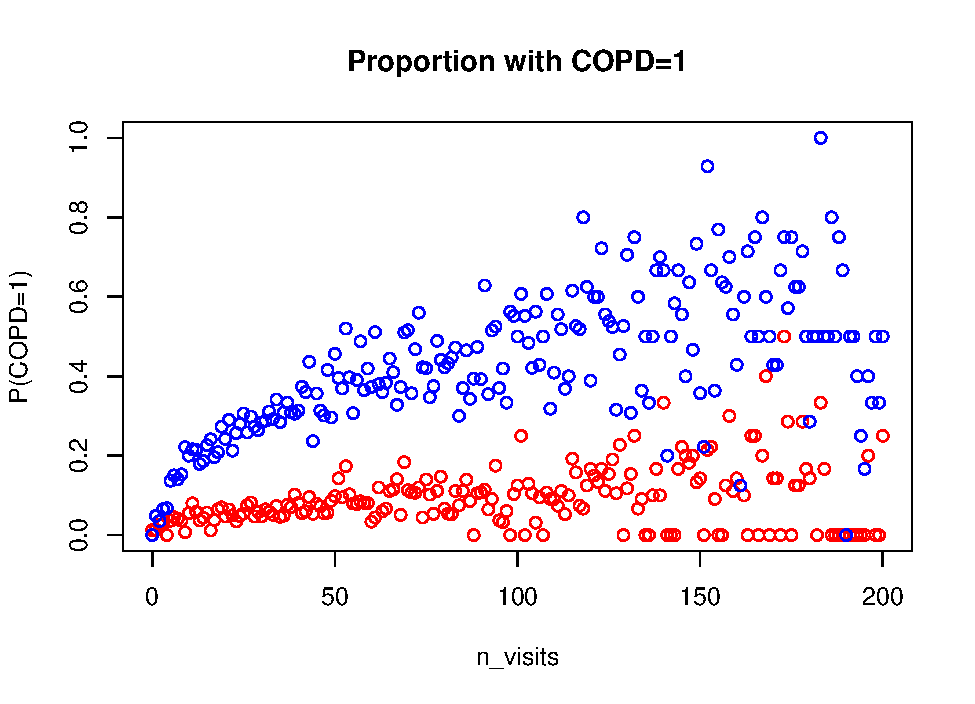
\includegraphics[width=.6\textwidth]{nvisits_scatternewCOPD200.pdf}
\end{center}

{\bf Next steps:} similarly code a new indicator for controls, see if it changes results. Generalize to other Charlson inputs (or other entirely new ICD codes), and look at ways to impute by incorporating n\_visits.

\pagebreak

Sample sizes for controls and cases for calculating the proportions in the above plots.

\begin{center}
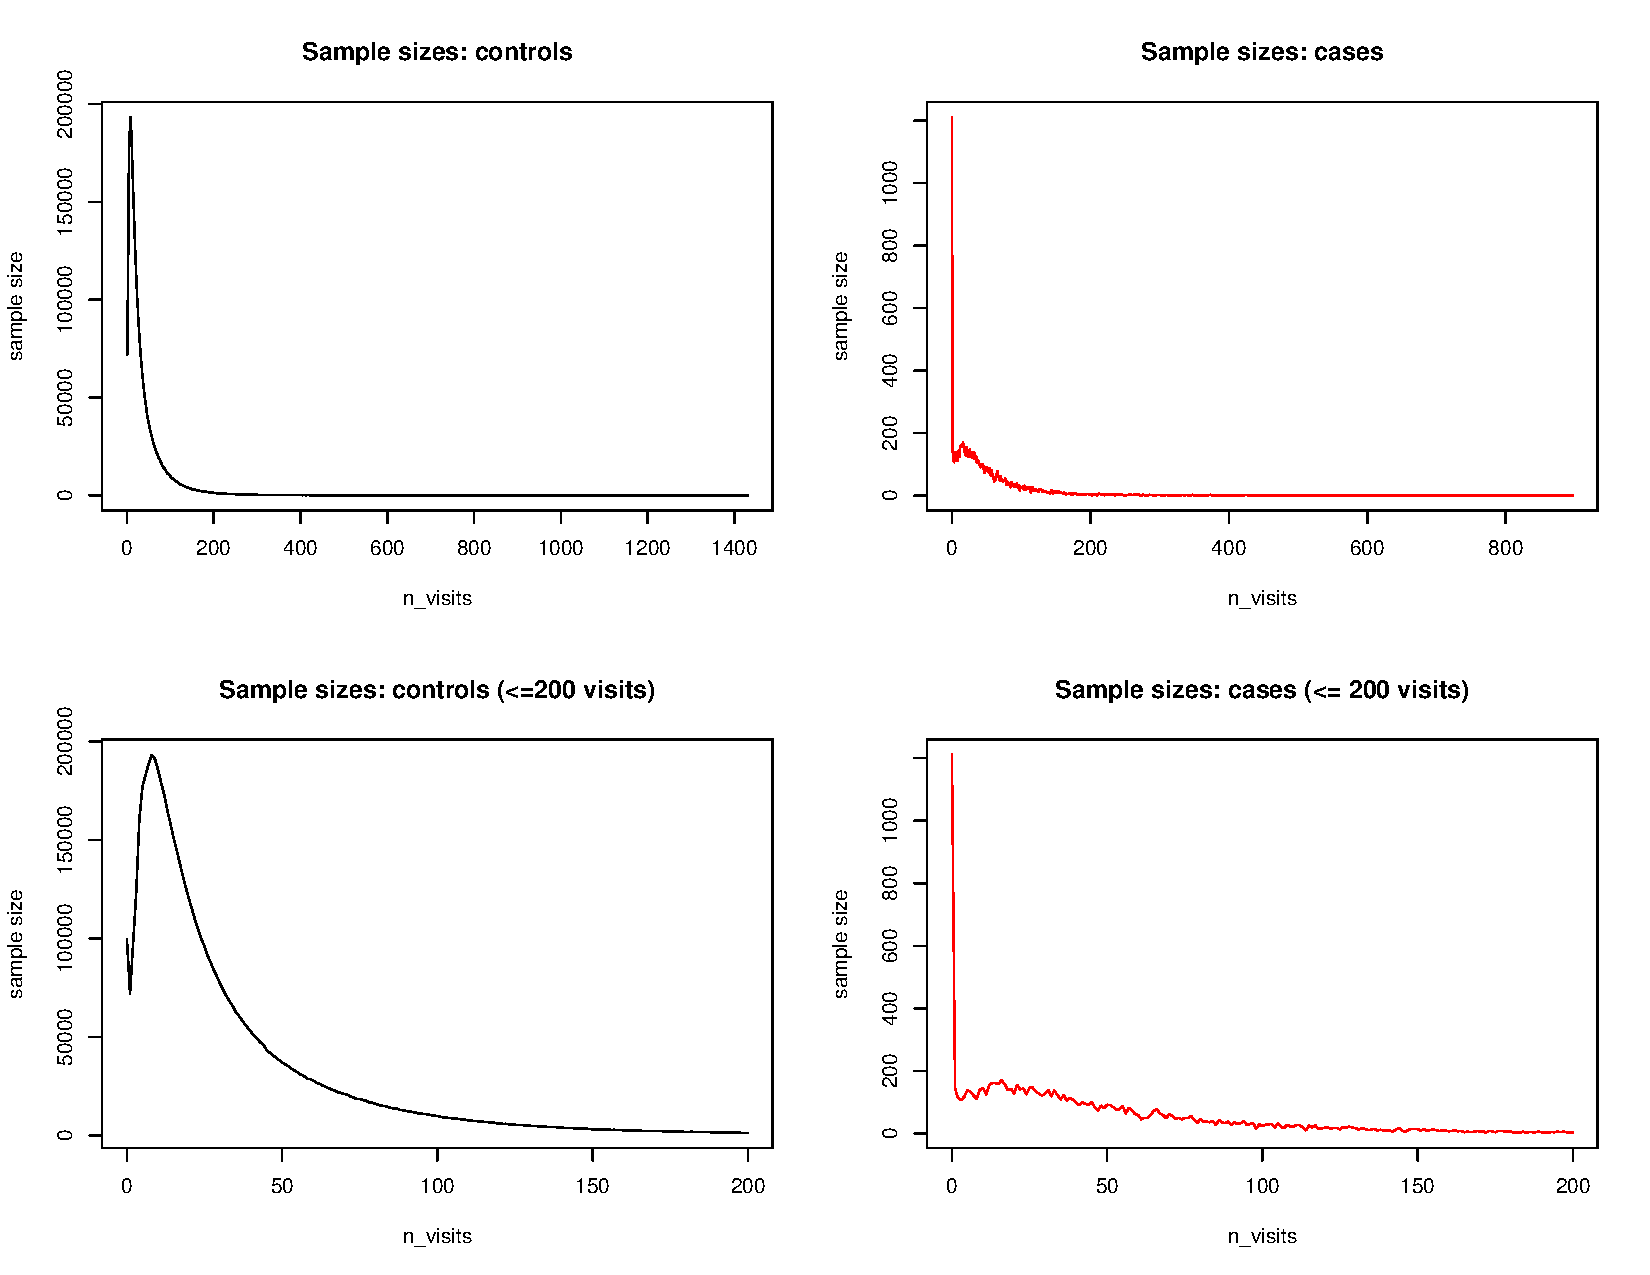
\includegraphics[width=\textwidth]{nvisits_samplesize.pdf}
\end{center}

\pagebreak
\subsubsection*{09/28 update}

\begin{itemize}
	\item Implemented new train/valid/test scheme
	\begin{itemize}
		\item Imputed records results are not exactly comparable
		\item Complete records results are comparable
	\end{itemize}
	\item Experimentation with regression imputation
	\item Experimentation with \texttt{xgboost} tuning parameters
	\item Currently working on multiple random sample with new train/valid/test scheme
\end{itemize}

\begin{table}[ht]
\centering
\begin{tabular}{lccc}
  \toprule
 & \textbf{Training AUC} & \textbf{Test AUC} & \textbf{Test AUC} \\
\textbf{Imputation method}& & \textbf{(imputed records)} & \textbf{(complete records)} \\
  \midrule
Separate class & 0.974 & 0.953 & 0.607 \\ 
 & (0.985) & (0.962) & (0.582) \\ \addlinespace
Median & 0.979 & 0.939 & 0.649 \\
   & (0.963) & (0.911) & (0.618) \\ \addlinespace
Regression & 0.952 & 0.739 & 0.770 \\ 
   & (0.911) & (0.750) & (0.798) \\ \addlinespace
1 rand. samp. & 0.987 & 0.783 & 0.890 \\
   & (0.916) & (0.780) & (0.833) \\  \addlinespace
   \midrule
   \multicolumn{4}{c}{10/04 update} \\
   \midrule
2 rand. samp. & 1.000 & 0.801 & 0.918 \\  \addlinespace
5 rand. samp. & 0.977 & 0.807 & 0.928 \\  \addlinespace
10 rand. samp. & 1.000 & 0.818 & 0.915 \\ 
   & (0.942) & (0.824) & (0.885) \\ \addlinespace
20 rand. samp. & 0.953 & 0.804 & 0.909 \\ 
   & (0.935) & (0.820) & (0.872) \\ \addlinespace
50 rand. samp. & 0.978 & 0.814 & 0.912 \\ \addlinespace
100 rand. samp. &  0.975 & 0.822 & 0.925 \\ 
   & (0.931) & (0.824) & (0.891) \\ 
   \bottomrule
\end{tabular}
   *all with \texttt{xgboost} prediction model; AUCs in parentheses 
   denote previous results.
\end{table}




\pagebreak
\subsubsection*{10/04 update}

\begin{itemize}
	\item Implemented new train/valid/test scheme with multiple imputation
	\item Updated table on previous page with result with multiple imputation
	\item Some improvement with a single random simpling imputation
	\item Some improvement compared to previous results, mostly for ``complete records'' test set
	\item Next step: utilize all of the data
\end{itemize}


\pagebreak
\subsubsection*{10/12 update}

\begin{itemize}
	\item Redo analysis with various Charlson variable treatments:
	\begin{itemize}
		\item no Charlson
		\item sampling from observed values (what was done previously)
		\item imputing a probability using number of visit (see Peter's proposed Geometric model)
		\item imputing by sampling using the fitted probability
	\end{itemize}
	\item Results:
	\begin{itemize}
		\item see table below
		\item dropping Charlson leads to a small decrease in testing performance for both imputed and ``complete'' records
		\item sampling with fitted probability has similar performance compared to the previous methods
		\item imputing the fitted probability leads to a huge improvement in performance
	\end{itemize}
	\item Currently examining where this large improvement comes from, still suspicious
	\item Try the same with multiple random samples
	\item Working on utilizing all data ...
\end{itemize}

\begin{table}[ht]
\centering
\begin{tabular}{lccc}
  \toprule
 & \textbf{Training AUC} & \textbf{Test AUC} & \textbf{Test AUC} \\
\textbf{Imputation method}& & \textbf{(imputed)} & \textbf{(complete)} \\
  \midrule
Separate class & 0.974 & 0.953 & 0.607 \\ \addlinespace
  Median & 0.990 & 0.941 & 0.674 \\ \addlinespace
  \multicolumn{4}{l}{\textbf{Simple random sample}} \\
  no Charlson & 0.988 & 0.771 & 0.873 \\ 
  random Charlson & 0.999 & 0.786 & 0.905 \\ 
  proba. Charlson & 1.000 & 0.906 & 0.975 \\ 
  proba.-weighted random Charlson & 0.997 & 0.795 & 0.896 \\ 
   \bottomrule
\end{tabular}
\end{table}




\pagebreak
\subsubsection*{10/26 update}

\textbf{Some follow-ups:}
\begin{itemize}
	\item Using number of visits to impute Charlson/GERD variables:
	\begin{itemize}
		\item Imputing probabilities is not a good idea as it is easy to spot missing values (between 0 and 1) from observed values (0/1)
		\item randomizing using the probability does not improve performance
		\item preferable to have a unified treatment
	\end{itemize}
	\item ICD codes reconding for cases comparing before and after
	\begin{itemize}
		\item we no longer see the large discrepancy between cases and control
		\item see COPD graphs below
	\end{itemize}
	\item Does the ``tv'' lab summaries contain some information about the number of measurements?
	\begin{itemize}
		\item there were some concern that variability would be associated with numer of measurements
		\item see density plots for ``chol'', ``hdl'' and ``trig'' below
		\item ``tv'' stands for ``total variation'' and is the average absolute  change between measurement (standardized by time between measurements)
		\item there does not seem to be strong associations
	\end{itemize}
\end{itemize}

\begin{center}
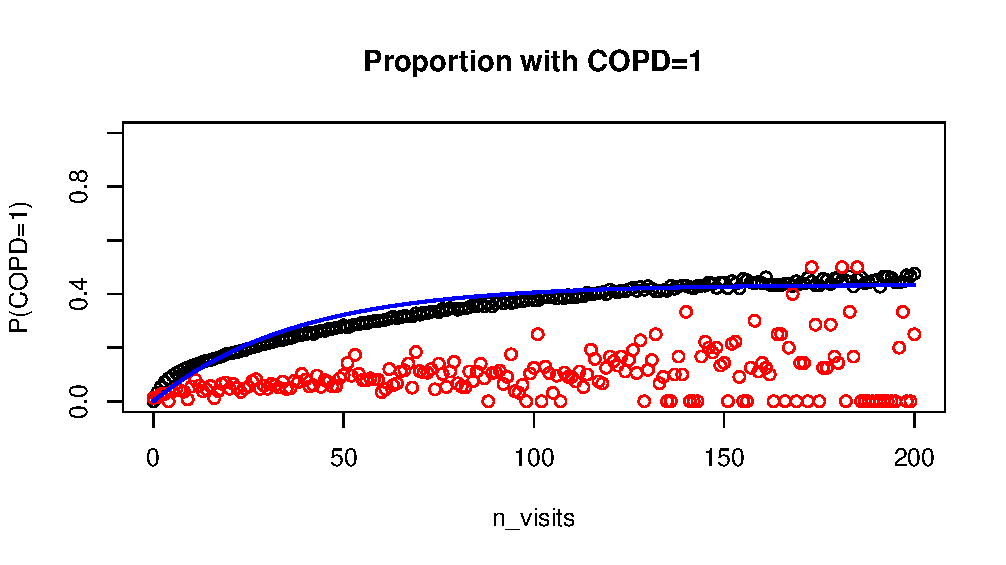
\includegraphics[width=.9\textwidth]{nvisits_scatterCOPD200.pdf}
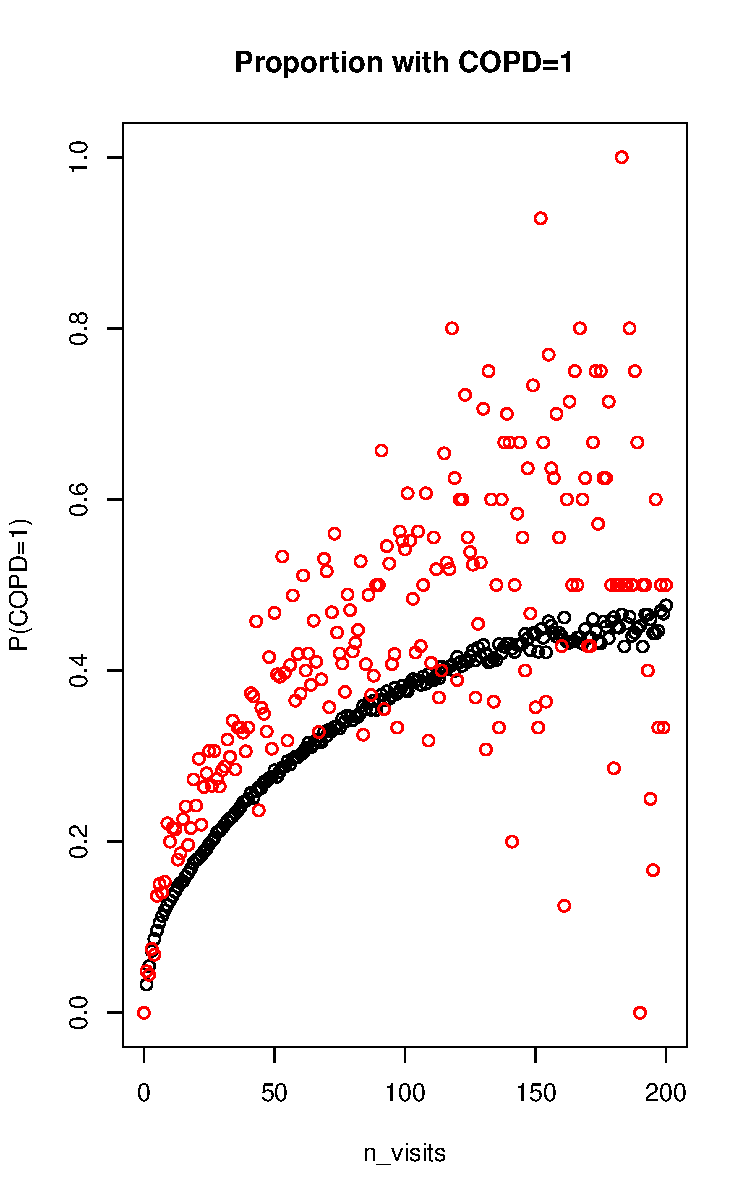
\includegraphics[width=.9\textwidth]{nvisits_scatterCOPDnew.pdf}
\end{center}




\begin{center}
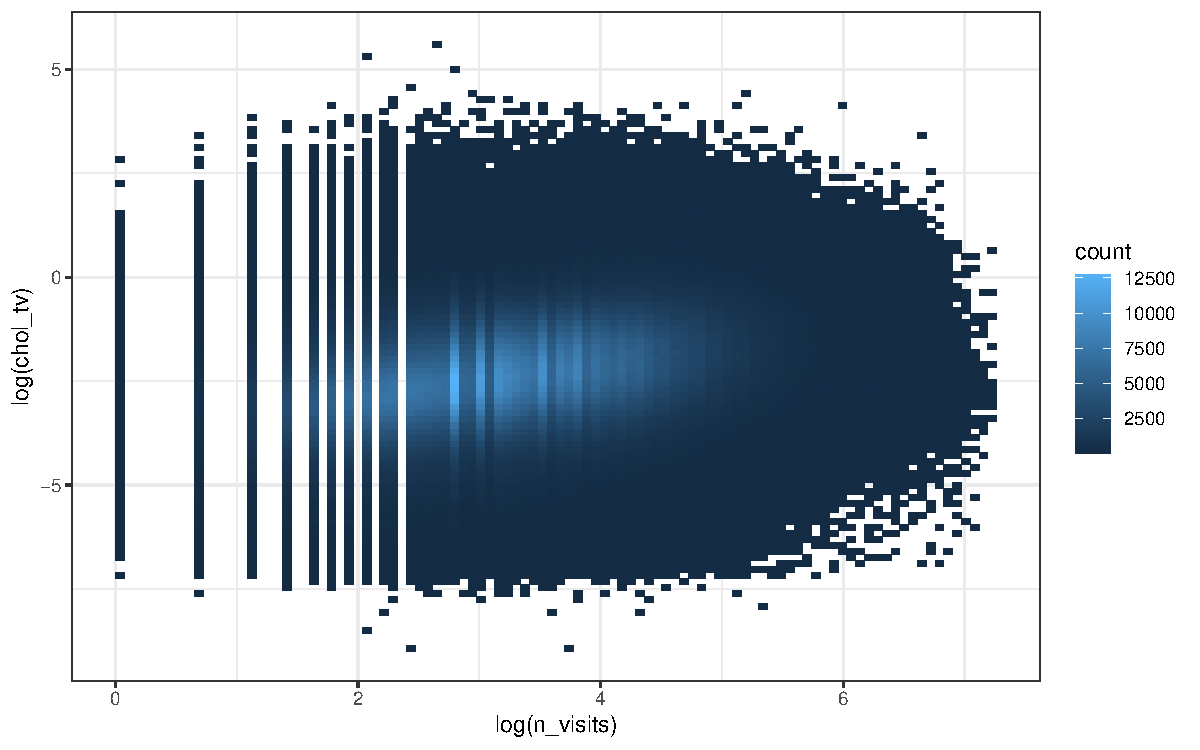
\includegraphics[width=.6\textwidth]{nvisits_chol_tv.pdf}
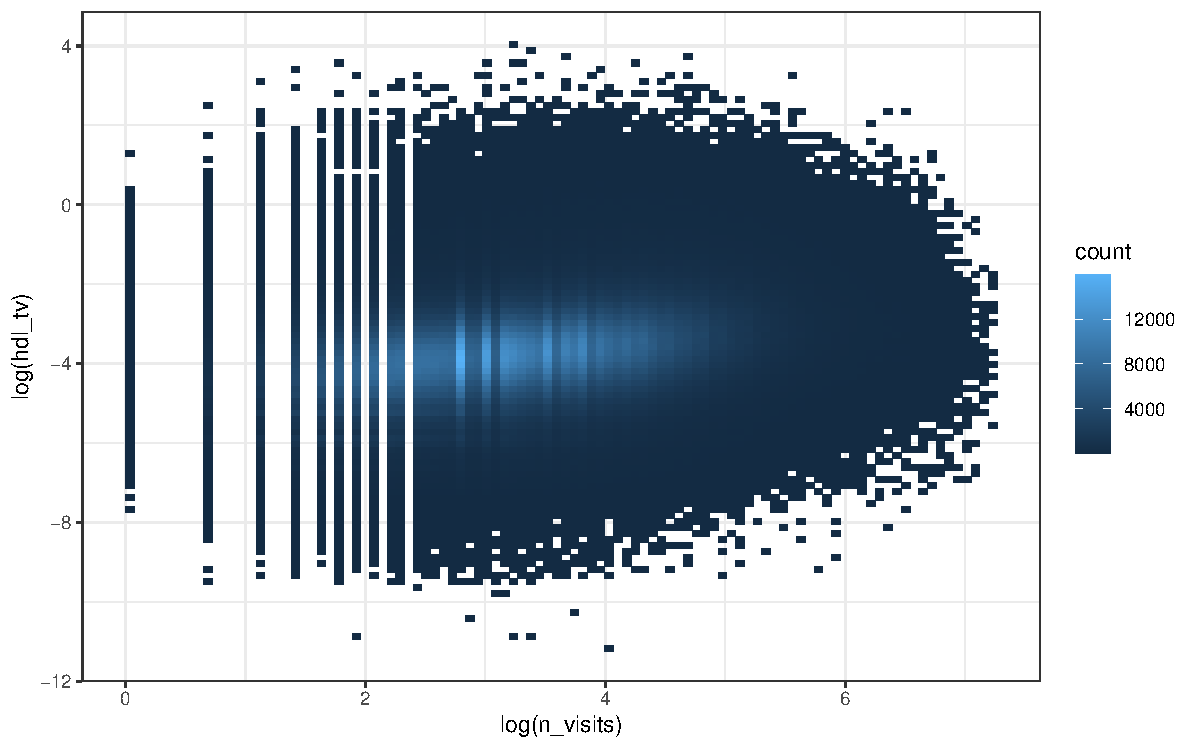
\includegraphics[width=.6\textwidth]{nvisits_hdl_tv.pdf}
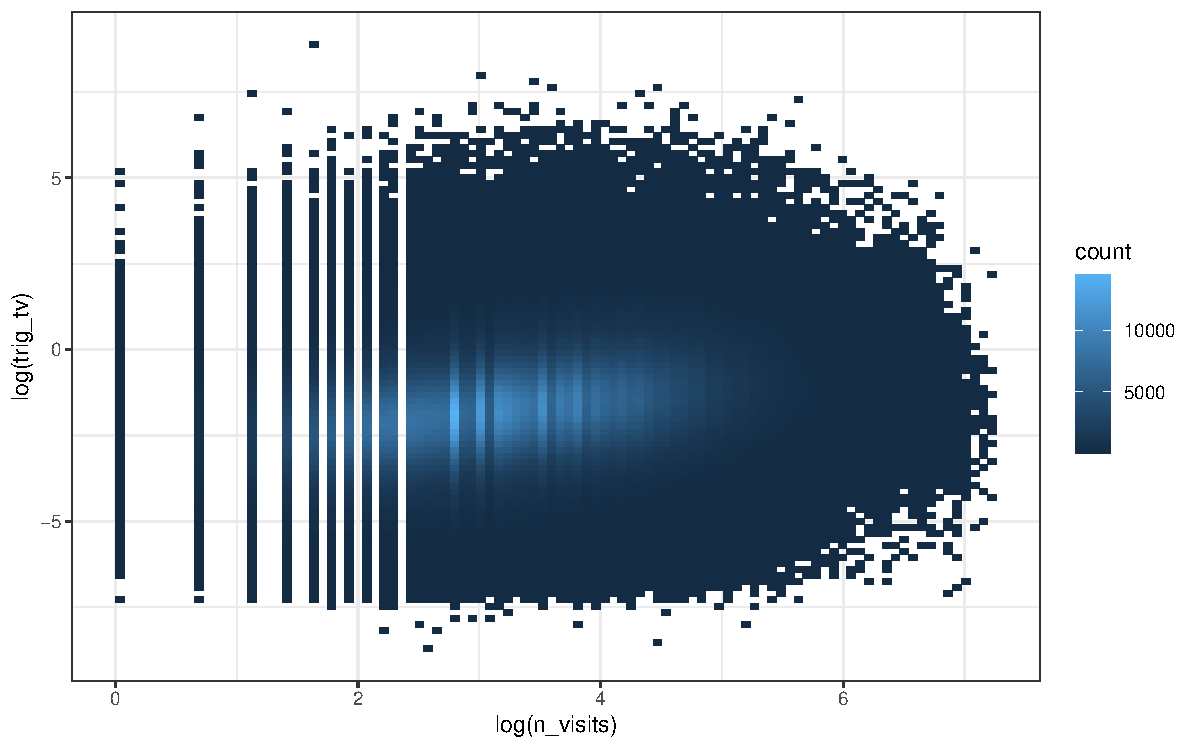
\includegraphics[width=.6\textwidth]{nvisits_trig_tv.pdf}
\end{center}

\newpage

\textbf{Using all data:}
\begin{itemize}
	\item Scalability study
	\item Sample 1M controls, keep all 11.4K cases (1M/11.4K)
	\item Train-test split 75-25 stratified
	\begin{itemize}
		\item Fixed test set (250K/2.8K)
		\item Training using increasing subsets of (750K/8.5K)
	\end{itemize}
	\item Working training set consisting of downsampling the controls
	\begin{itemize}
		\item $n=$10K, 20K, 50K, 100K
		\item keeping all 8.5K cases
		\item as $n$ increases, the training set becomes more and more unbalanced
		\item $n=$10K is close to balanced
	\end{itemize}
	\item Validation set: stratified 2-1
	\begin{itemize}
		\item Model/imputation trained on 67\%, validation/model selection on 33\%
	\end{itemize}
	\item Extra testing set: ``complete cases'' (same as before, 710/290)
	\begin{itemize}
		\item small, with possible overlap 
		\item not a super reliable testing set
	\end{itemize}
	\item Methods (e.g. with 100K/8.5K $\to$ 66.7K/5.7K)
	\begin{itemize}
		\item Unweighted: do nothing special
		\item Downsample: sample controls to get a balance training set (5.7K/5.7K)
		\item Resample: resample cases to get a balance training set (66.7K/66.7K)
		\item Weighted: cases' loss reweighted by $w=66.7/5.7$
		\item Weighted\_ sqrt: by $\sqrt(w)$
		\item Weighted\_ sq: by $w^2$
	\end{itemize}
\end{itemize}

\begin{center}
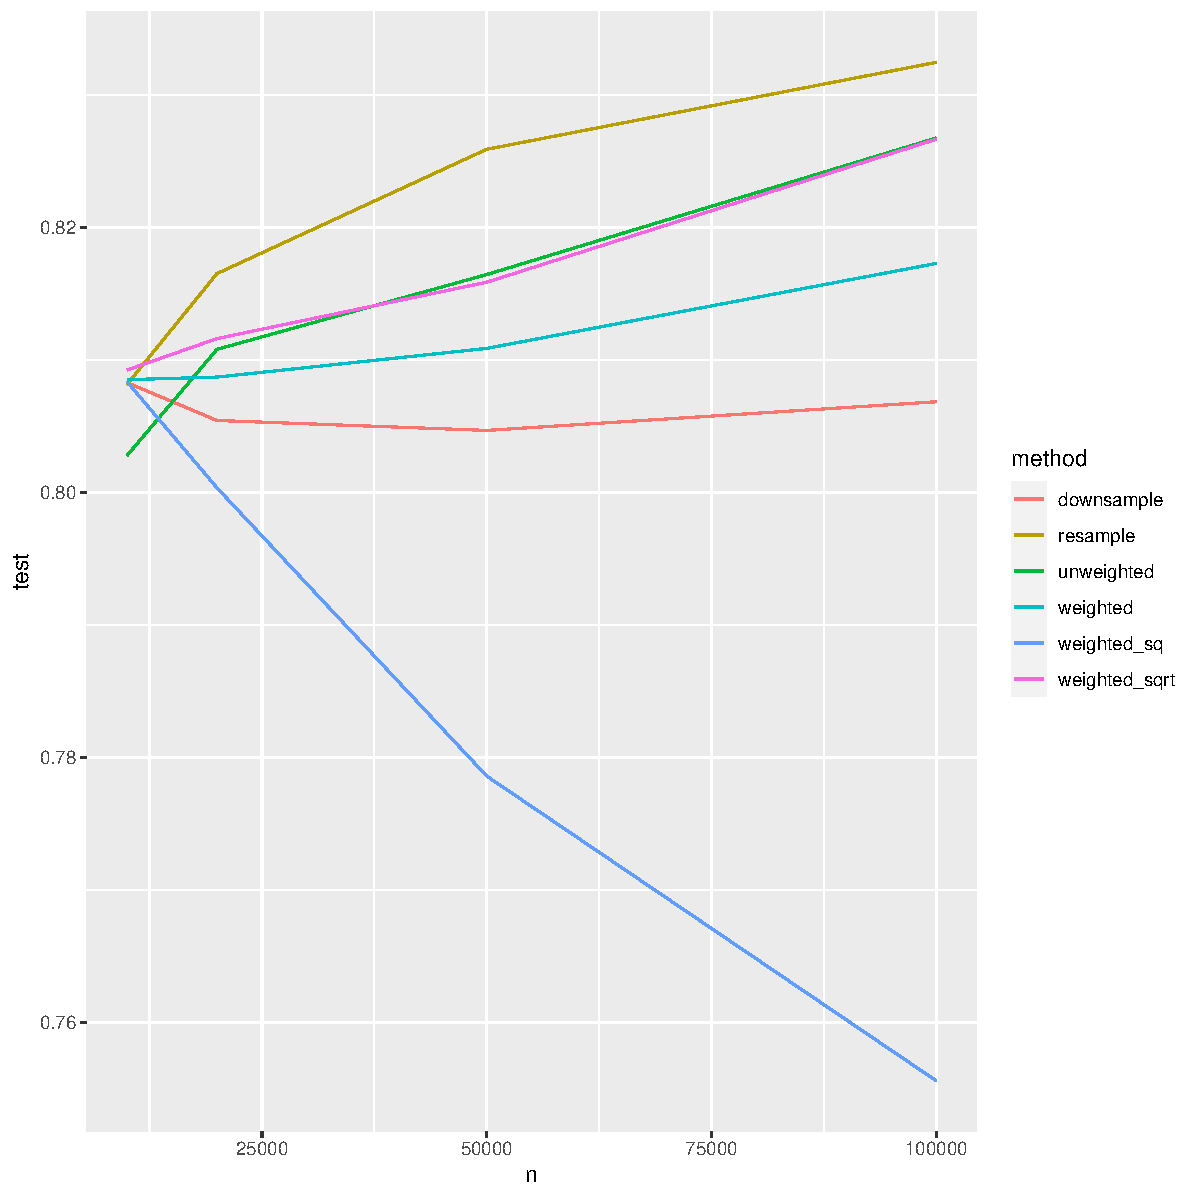
\includegraphics[width=.9\textwidth]{aucs_large_test.pdf}
\end{center}

\begin{center}
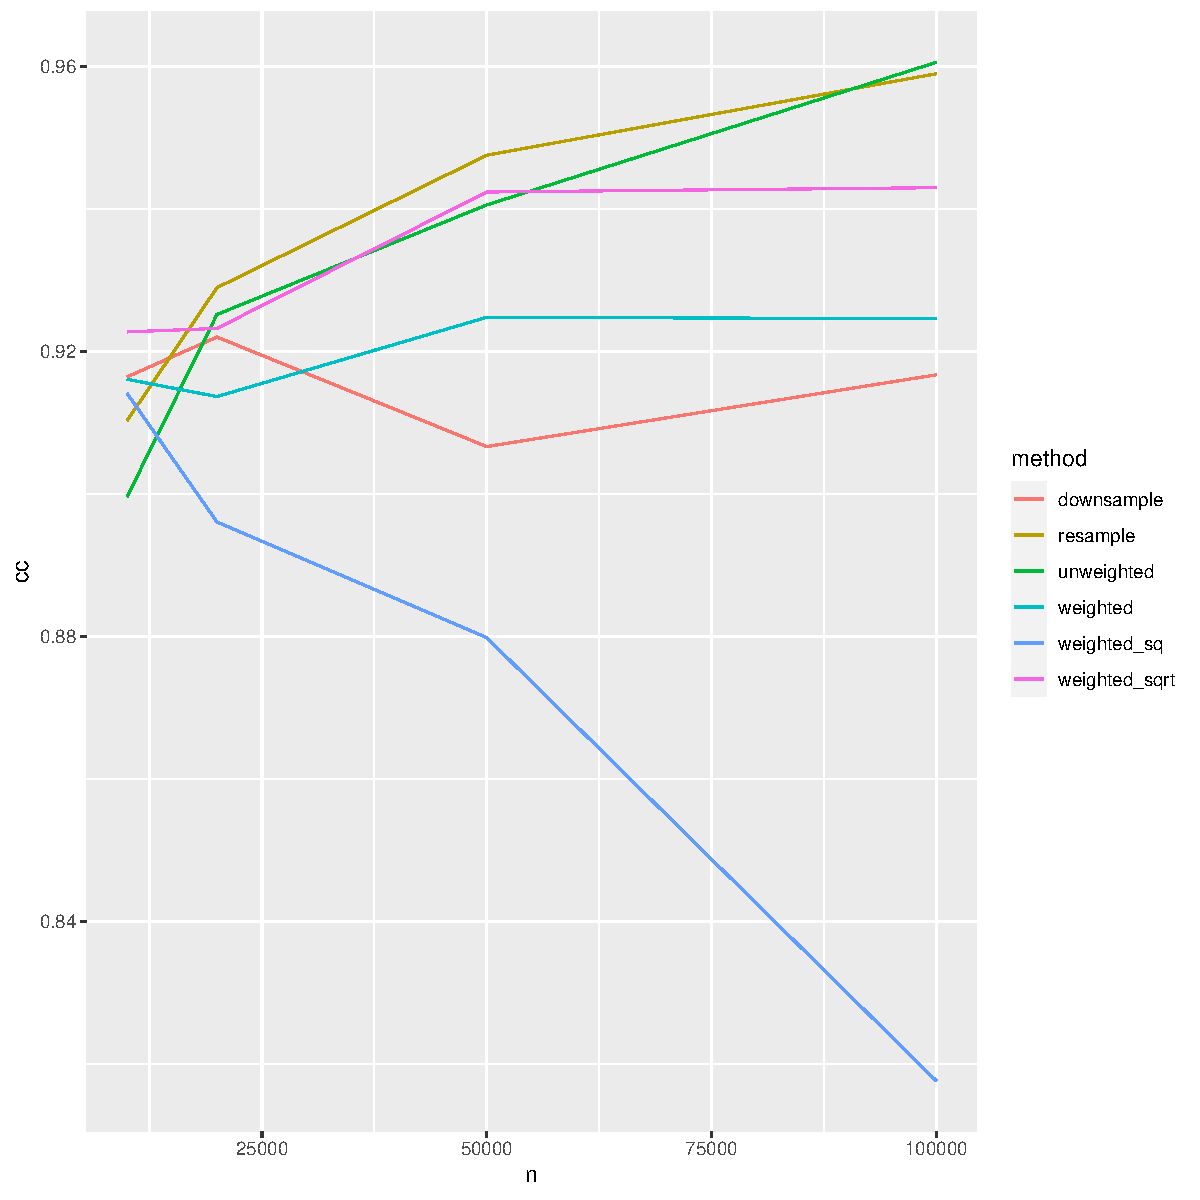
\includegraphics[width=.9\textwidth]{aucs_large.pdf}
\end{center}




\pagebreak
\subsubsection*{11/02 update}


\subsubsection*{Tuning}

\begin{itemize}
	\item subsampling each iteration, learning rate, tree depth
	\item Some improvement is still possible
	\item Dependent on the training set size
	\begin{itemize}
		\item Tuned on small smaple size, improvments don't necessarly carry to larger sample size
		\item prohibitive to tune on large dataset
	\end{itemize}
\end{itemize}


\subsubsection*{Training set size}

\begin{itemize}
	\item Training becomes \textit{very} slow
	\item Early results show improvement beyond 100K
	\item Exploring ways to speed up training (lightgbm, catboost)
\end{itemize}



\newpage
\begin{center}
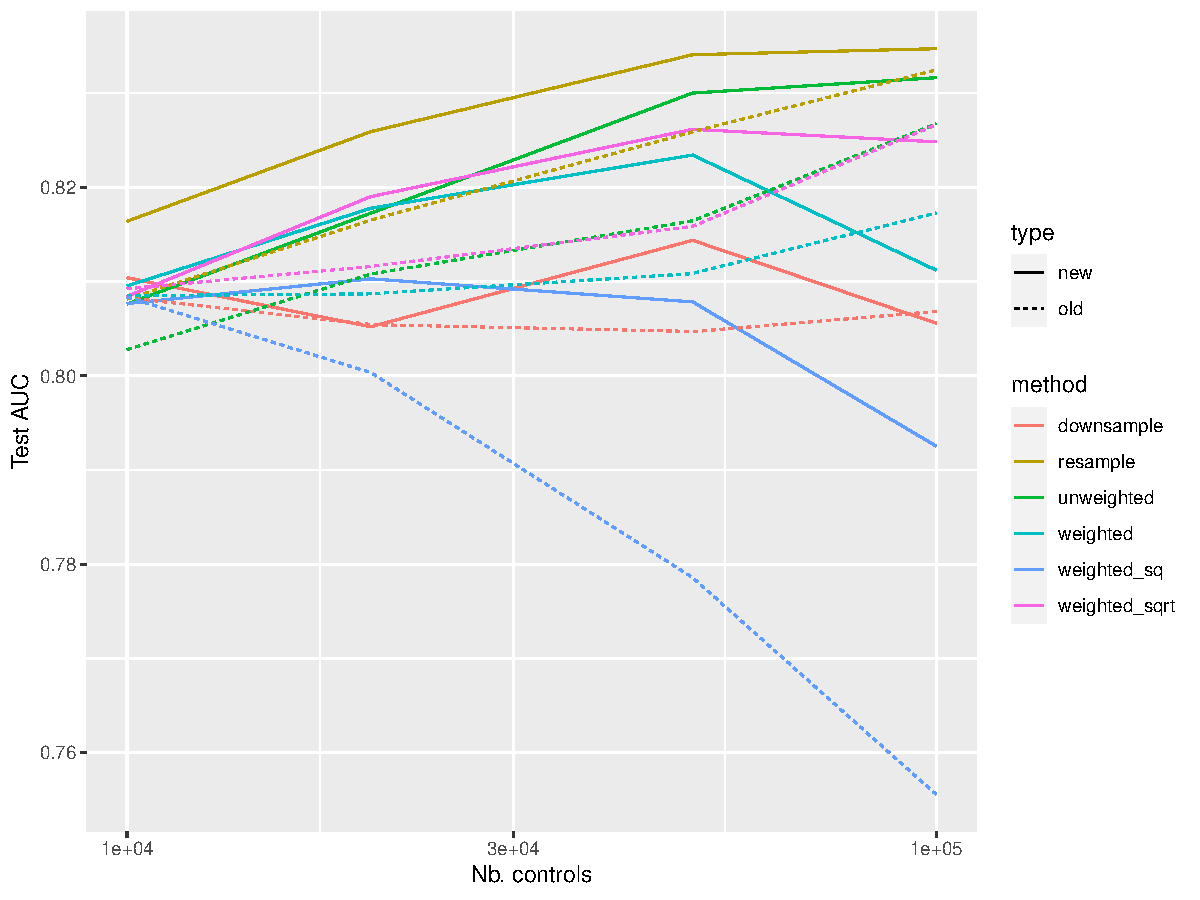
\includegraphics[width=.9\textwidth]{aucs_large_test_new.pdf}
\end{center}

\begin{center}
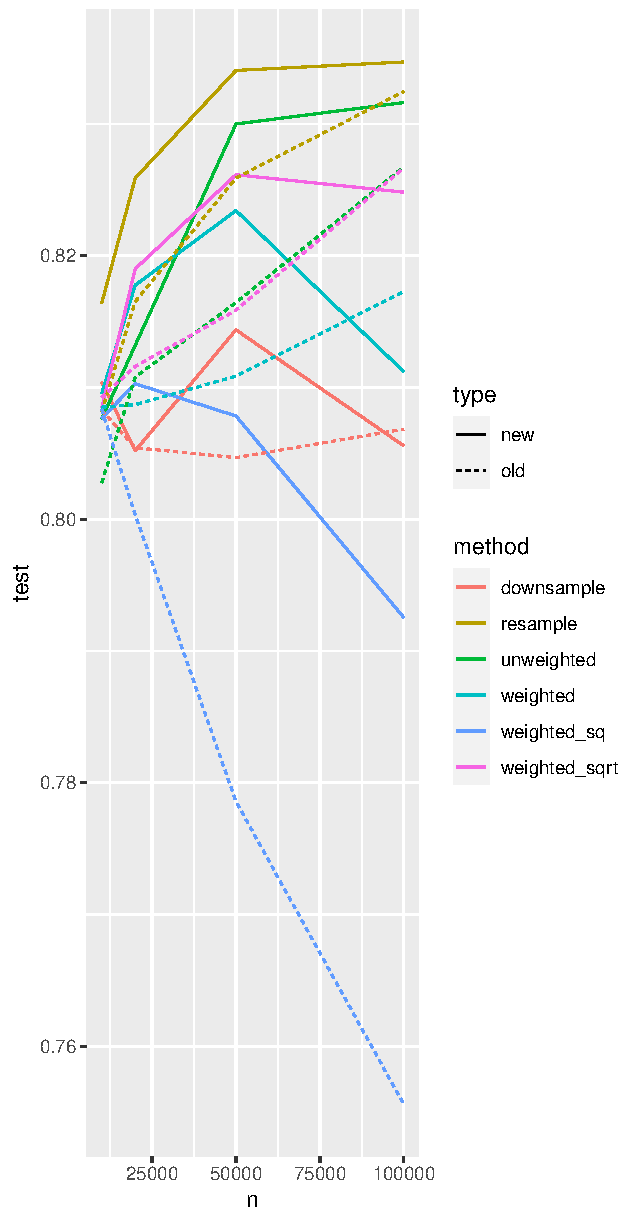
\includegraphics[width=.9\textwidth]{aucs_large_cc_new.pdf}
\end{center}



\pagebreak
\subsubsection*{11/09 update}

\subsubsection*{Training set size}

\begin{itemize}
	\item Added results for $>100K$ controls
	\item Goal:
	\begin{itemize}
		\item Harness all data
		\item Study how the increasing case/control imbalance affects results
	\end{itemize}
	\item Similar train/valid/test split as before
	\begin{itemize}
		\item 2M control + 11K cases (increased from 1M previously to allow the 1M case)
		\item All splits are stratified (cases/control proportion preserved)
		\item test: 25\%, train+valid: 75\%
		\item $N$: number of controls in train+valid
		\item subsample train+valid controls down to $N$
		\item train: 67\%, valid: 33\%
		\item NB: test set is fixed with $N$, validation set increases with $N$
	\end{itemize}
	\item Imputation:
	\begin{itemize}
		\item Simple random sampling from the training set into validation and testing sets
	\end{itemize}
	\item \texttt{xgboost} parameters:
	\begin{itemize}
		\item Default values, except:
		\item \texttt{subsample = 0.5}
		\item \texttt{max\_depth = 5}
		\item \texttt{eta = 0.5} (stepsize)
		\item NB: these values are represented with vertical dashed lines in the following ``Tuning'' section
	\end{itemize}
	\item Methods:
	\begin{description}
		\item[downsample] sample controls down to the number of cases
		\item[resample] sample (w/ replacement) the cases up to the number of controls (note that controls appearing more than once get different imputation)
		\item[unweighted] no resample, no reweighting
		\item[weighted] no resampling, cases upweighted by $n_{\text{controls}} / n_{\text{cases}}$
		\item[weighted\_sqrt] no resampling, cases upweighted by $\sqrt{n_{\text{controls}} / n_{\text{cases}}}$
		\item[weighted\_sq] no resampling, cases upweighted by $(n_{\text{controls}} / n_{\text{cases}})^2$ (dropped from graph because much worse values and changed the scale too much to see others well)
	\end{description}
	\item Plots:
	\begin{itemize}
		\item y-axis: Test set AUC and Validation set AUC
		\item x-axis: Nb. of controls before train/valid split
		\item colors: which method is used to deal with imbalance
		\item linetype: new vs. old tuning. The new tuning was performed manually with 100K controls; the old tuning with 10K controls. For more on tuning, see next section.
	\end{itemize}
	\item Results and analysis:
	\begin{itemize}
		\item Single repetition, so there is some variablity due to the sampling. To get a sense of the scale of the variability, the ``downsample'' method should be the same across the range. I might do multiple repititions in the future, but this gets very long for large $N$, so I am avoiding it for now.
		\item The ``resampling'' method seems to be the best across the board
		\item The ``unweighted'' method seems more stable?
		\item Not much to gain beyond 50K-100K (decrease? within variability?). The best tuning parameters might not be the same for larger datasets, as is apparent between old/new tuning curves.
	\end{itemize}
\end{itemize}

\begin{center}
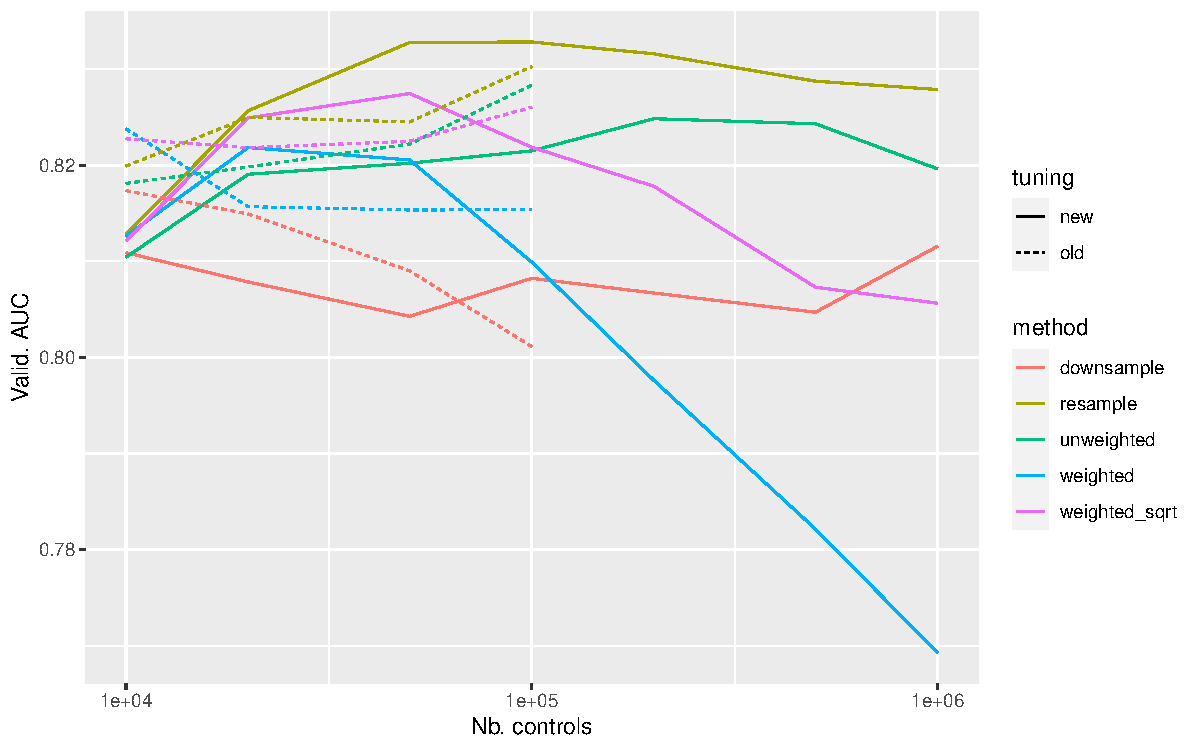
\includegraphics[width=.9\textwidth]{best_aucs_large_valid.pdf}
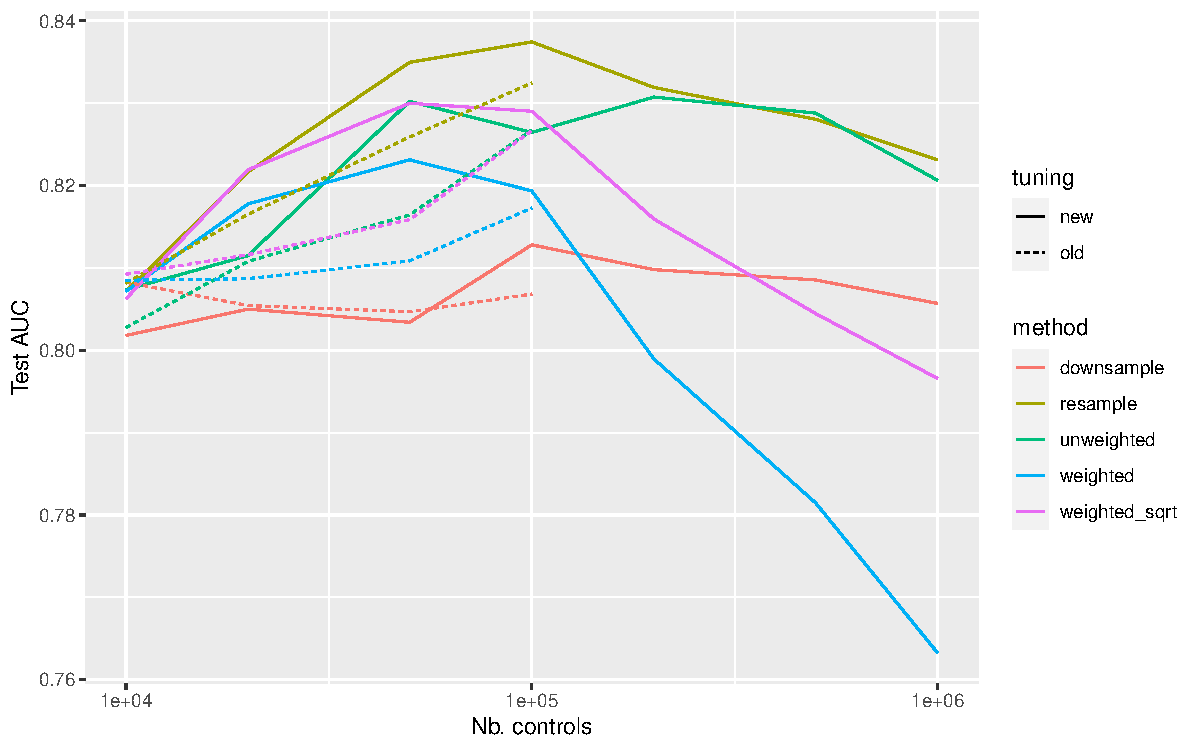
\includegraphics[width=.9\textwidth]{best_aucs_large_test.pdf}
\end{center}

\pagebreak
\subsubsection*{Tuning}

\begin{itemize}
	\item Protocol:
	\begin{itemize}
		\item Same as above, except:
		\begin{itemize}
			\item Fix Nb. controls to $N=100K$
			\item Use ``resample'' method only
		\end{itemize}
		\item Fix all parameters to their default value stated above (and blotted with a vertical dashed line), vary one parameter along a plausible range
	\end{itemize}
	\item Parameters:
		\begin{description}
			\item[max\_depth] Control the complexity of the tree added at each iteration (deeper trees have more explanatory power, but can overfit)
			\item[subsample] Determines what percetage of the training set is used to fit the next tree (more subsampling prevents overfitting but slows down fitting and may lead to under-fitting)
			\item[eta] (step-size) controls how much the new tree contributes to the model (small step-size prevents overfitting, but slows down fitting)
		\end{description}
	\item Results and analysis:
	\begin{description}
		\item[max\_depth] Above depth 4-5, not much variation on valid/test AUCs; some improvment on train/cc AUCs
		\item[subsample] Except for small proportions, not much variation for all 4 datasets; best seems to be around 0.4-0.75
		\item[eta] waiting for results ...
	\end{description}
\end{itemize}


\subsubsection*{Next steps}

\begin{itemize}
	\item Tuning for larger number of controls
	\item Alternative metrics
\end{itemize}


\begin{center}
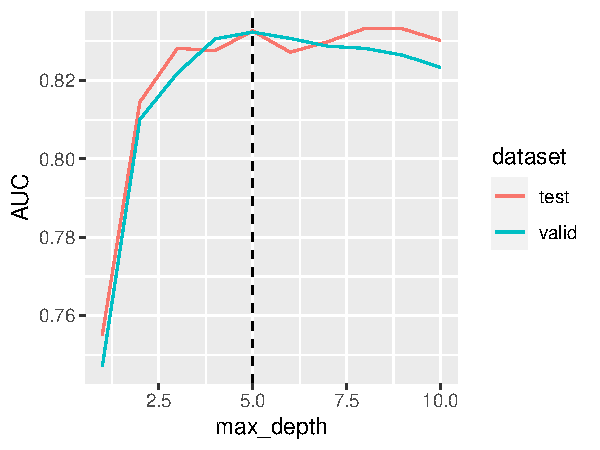
\includegraphics[width=.9\textwidth]{best_aucs_tuning_max_depth.pdf}
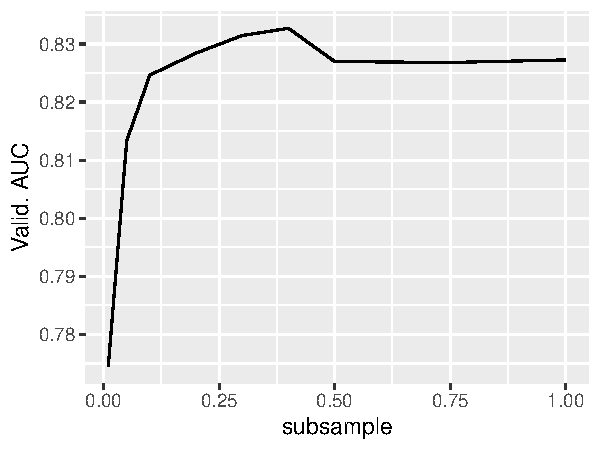
\includegraphics[width=.9\textwidth]{best_aucs_tuning_subsample.pdf}
\end{center}



\pagebreak
\subsubsection*{11/16/2021 update}

\textbf{Tuning:}
\begin{itemize}
	\item AUROC, N=100K controls
	\item step-size: added results, see graph below
	\item for small eta, I didn't reach the stopping criterion, so take results with a grain of salt
	\item Seems like the ``default'' values I was using were mostly good
	\item Working on N=1M (\textit{very slow...})
\end{itemize}

\textbf{Multiple tests sets:}
\begin{itemize}
	\item All: original test set
	\item Complete cases: subset to only complete observations
	\item x-y\% missing: subset to observations with (x,y]\% of missing values
	\item AUROC graph below (resmapling cases):
	\begin{itemize}
		\item Seems to stabilize beyond 100K
		\item 10-30\% missing values have much larger AUC
		\item Complete cases is much more variable since smaller
	\end{itemize}
\end{itemize}
\begin{table}[ht]
\centering
\begin{tabular}{lrrr}
  \toprule
\textbf{Test set} & \textbf{Sample size} & \textbf{Nb. cases}& \textbf{\% cases} \\
  \midrule
All & 502849 & 2849 & 0.56\%  \\ \addlinespace
Complete cases & 1571 & 12 & 0.76\%  \\ \addlinespace
0-5\% missing & 83640 & 286 & 0.34\%  \\ \addlinespace
5-10\% missing & 133194 & 369 & 0.28\%  \\ \addlinespace
10-30\% missing & 163377 & 1122 & 0.69\%  \\ \addlinespace
30-100\% missing & 121067 & 1060 & 0.86\%  \\
   \bottomrule
\end{tabular}
\end{table}

\textbf{Metrics:}
\begin{itemize}
	\item AUC ROC: area under the ROC curve (sens, 1-spec)
	\item AUC PRC: area under the precision-recall curve (prec, rec)
	\item TPR: true positive rate (\textit{recall, sensitivity}, TP/P, ``\% of cases that would be tested'')
	\item PPV: positive predictive value (\textit{precision}, TP/DP, ``\% of cases among those tested''
	\item Detection prevalance: (DP/N, ``\% of patients tested'')
\end{itemize}

\pagebreak
\begin{center}
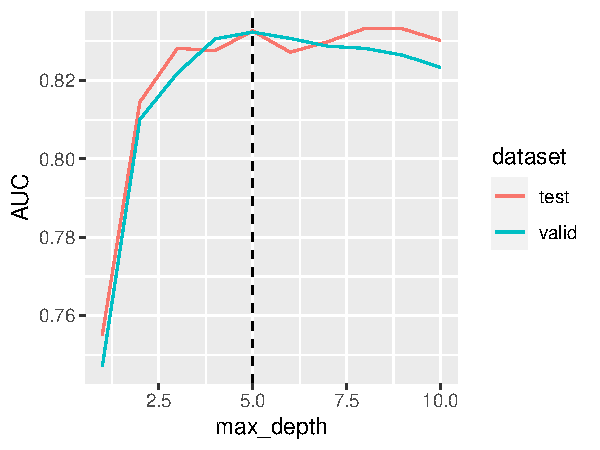
\includegraphics[width=.7\textwidth]{best_aucs_tuning_max_depth.pdf}
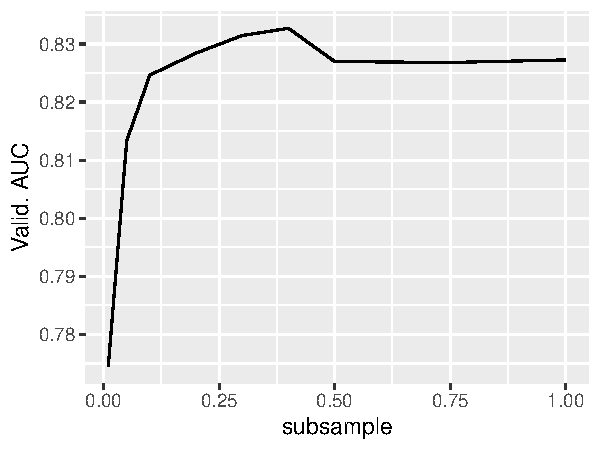
\includegraphics[width=.7\textwidth]{best_aucs_tuning_subsample.pdf}
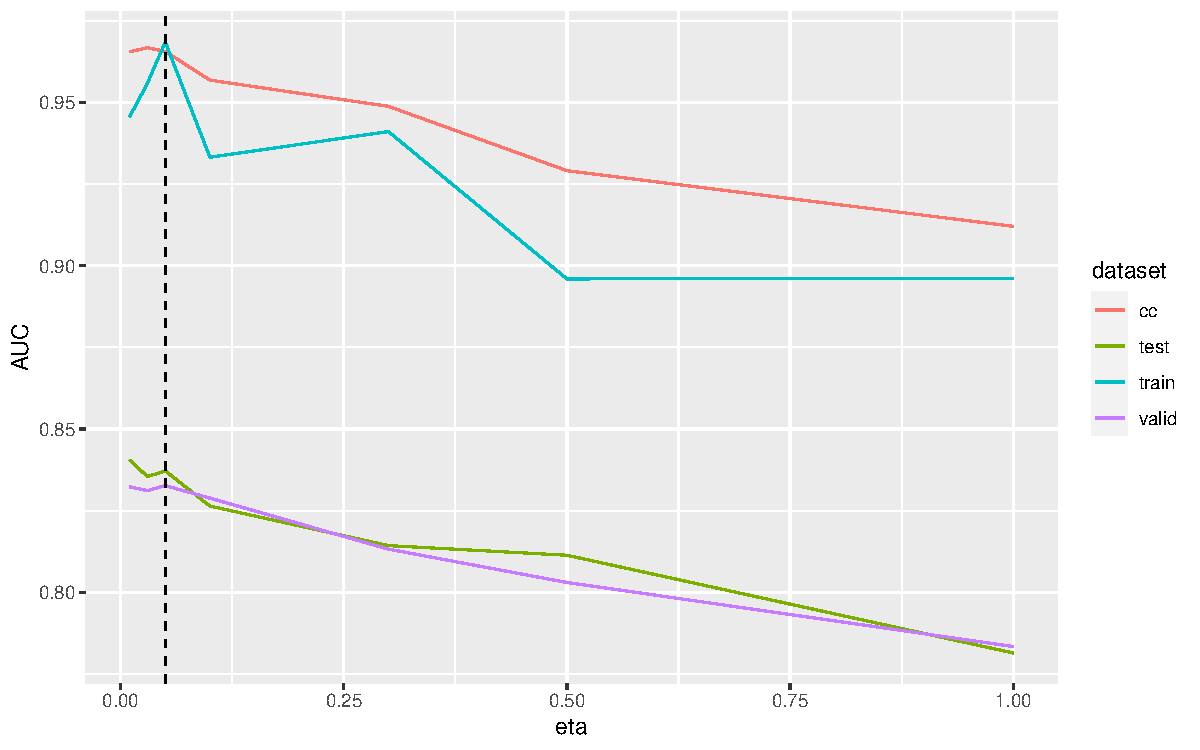
\includegraphics[width=.7\textwidth]{best_aucs_tuning_eta.pdf}
\end{center}


\pagebreak
\begin{center}
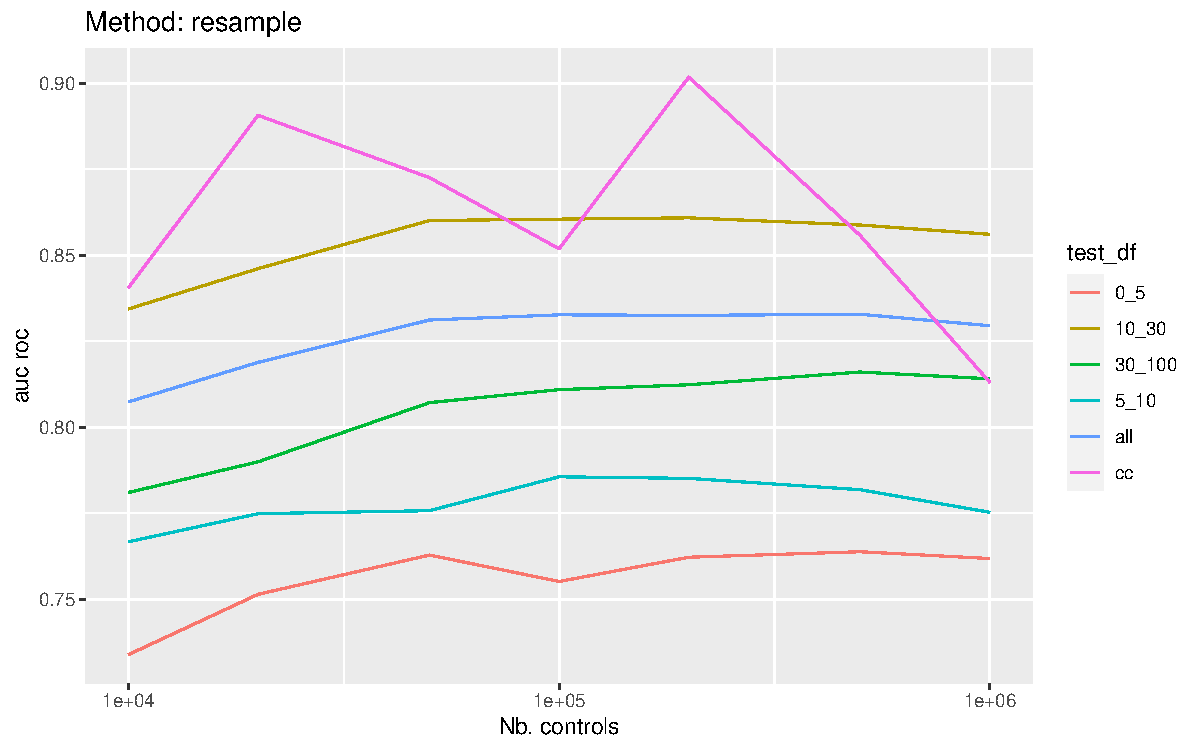
\includegraphics[width=.9\textwidth]{size_resample_roc.pdf}
\end{center}


\pagebreak
\begin{center}
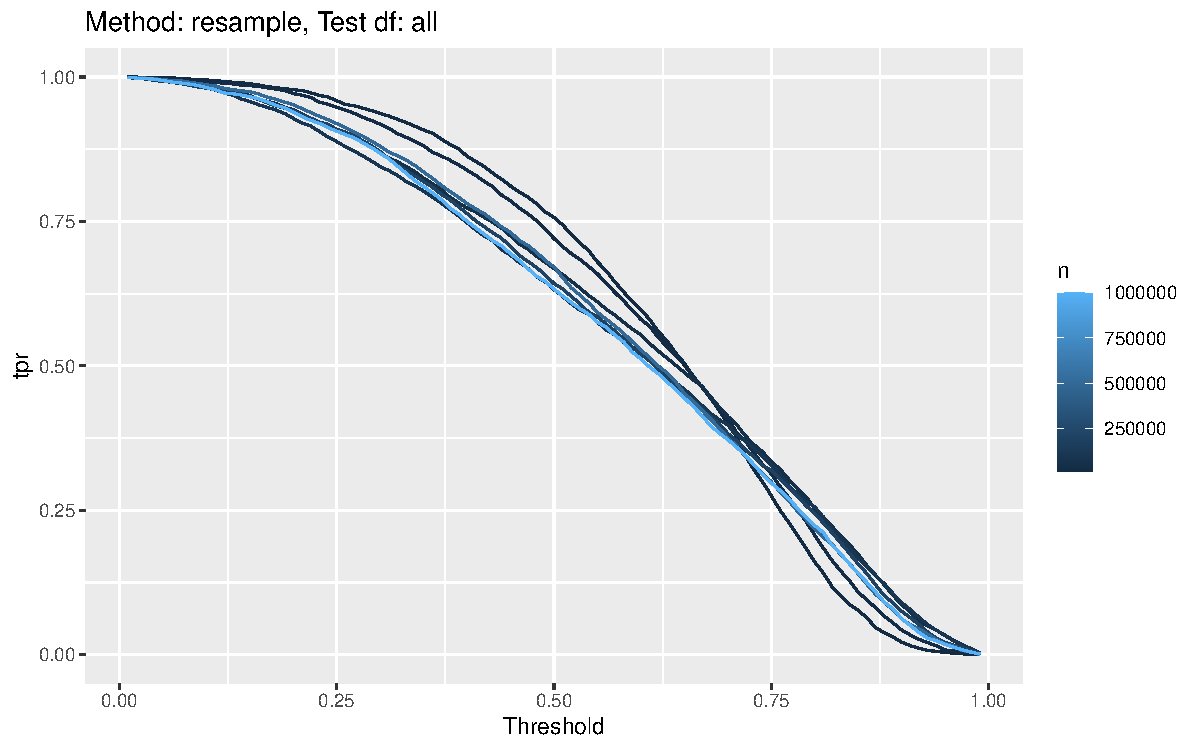
\includegraphics[width=.7\textwidth]{size_resample_all_tpr.pdf}
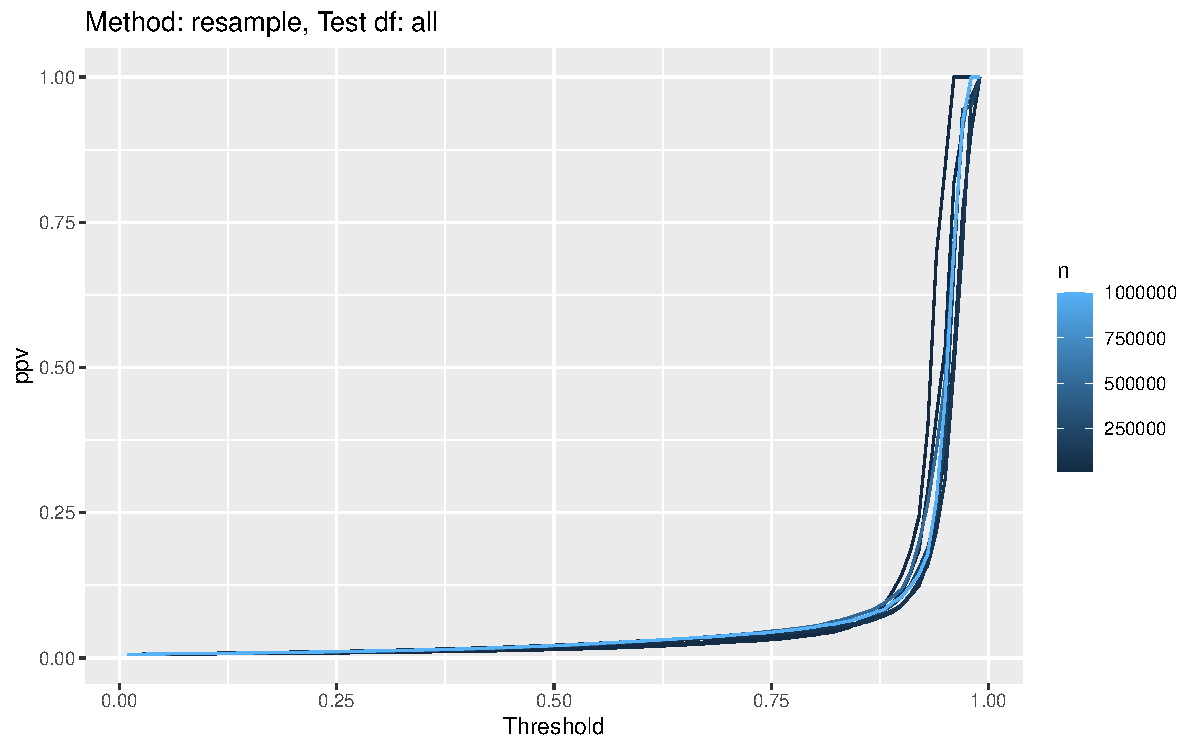
\includegraphics[width=.7\textwidth]{size_resample_all_ppv.pdf}
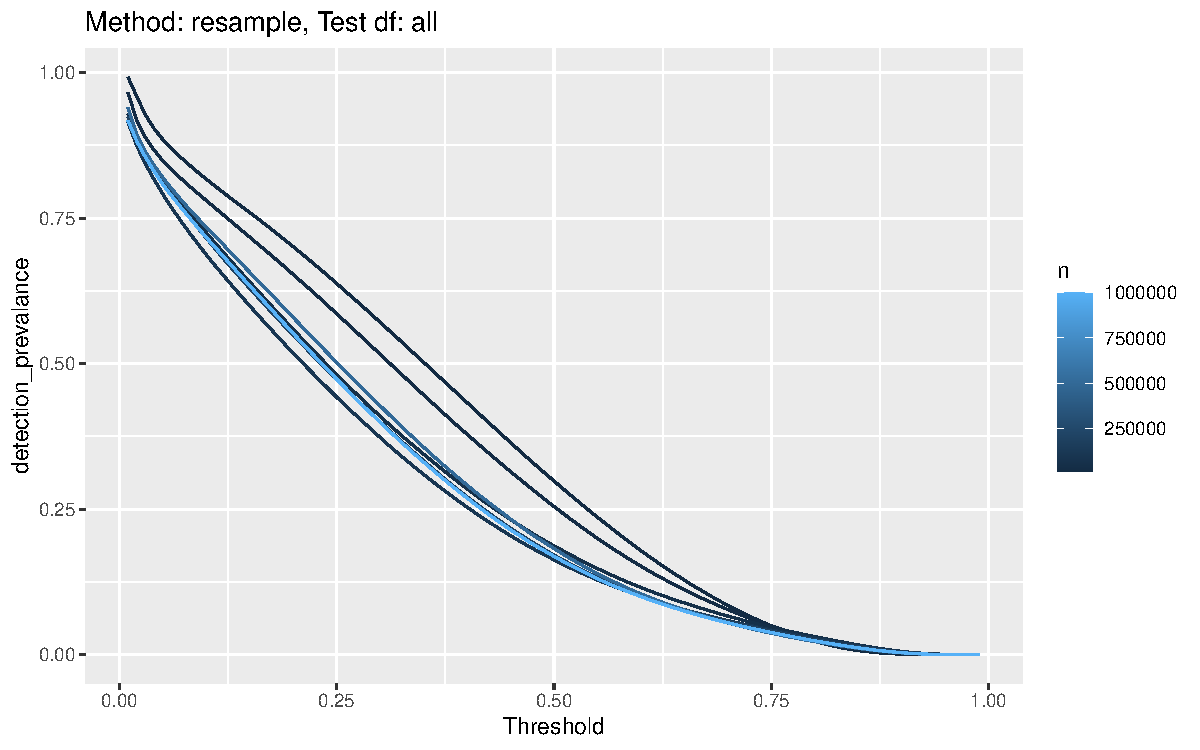
\includegraphics[width=.7\textwidth]{size_resample_all_detection_prevalance.pdf}
\end{center}


\pagebreak
\begin{center}
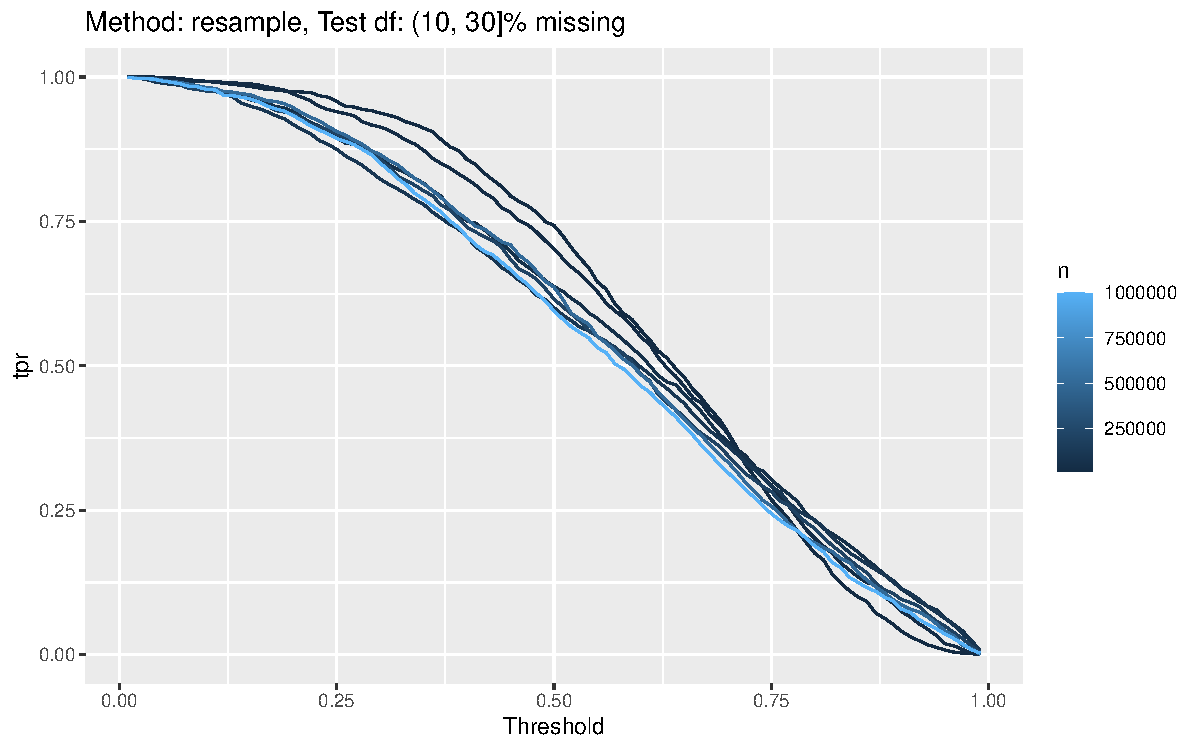
\includegraphics[width=.7\textwidth]{size_resample_1030missing_tpr.pdf}
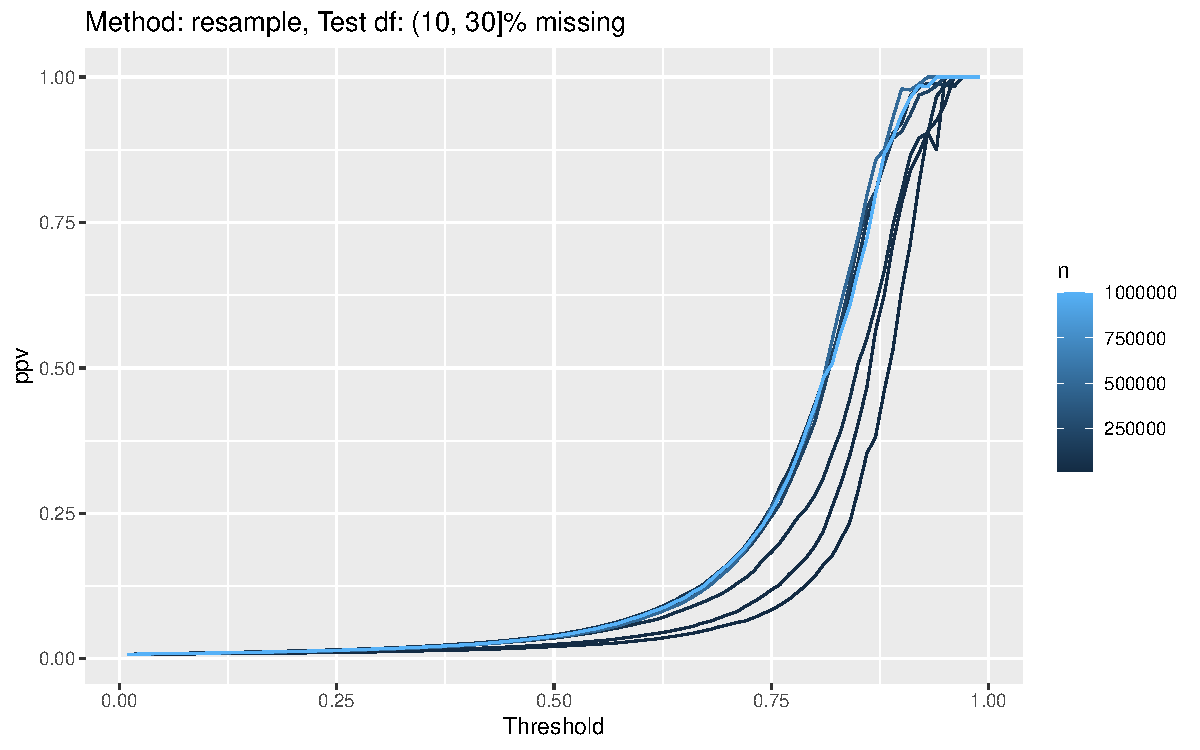
\includegraphics[width=.7\textwidth]{size_resample_1030missing_ppv.pdf}
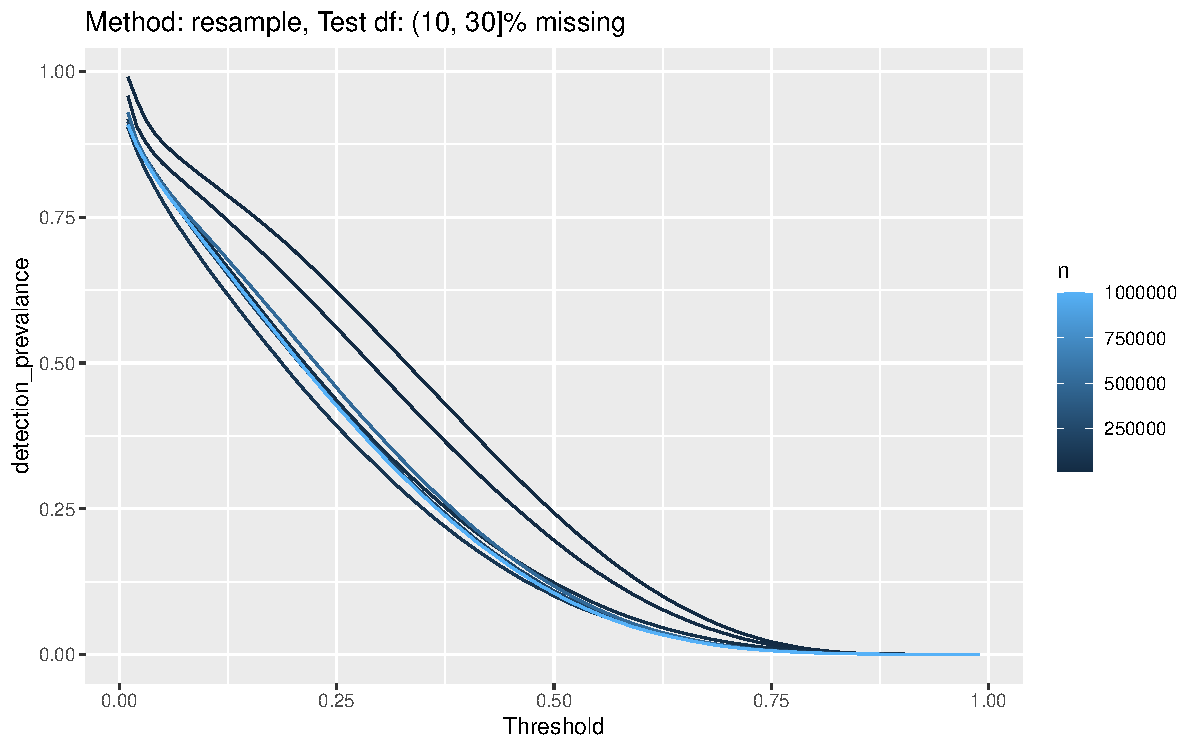
\includegraphics[width=.7\textwidth]{size_resample_1030missing_detection_prevalance.pdf}
\end{center}



\pagebreak
\subsubsection*{11/23/2021 update}

\paragraph*{Missing values}
	\begin{itemize}
		\item Last week: split test set by proportion of missing values
		\item New: split test set by proportion of missing values within groups of variables
		\item Better for: 10-30\% of missing values, 14-33\% of missing lab variables, missing smoking variables
		\item Worse for: 0-10\% of missing values, 1-100\% missing charlson variables, 0-6 and 100\% missing lab variables
		\item NB: high case \% for missing charlson scores (but smaller total observations); higher case \% for 100\% missing lab variables
	\end{itemize}

\paragraph*{Calibration}

\begin{itemize}
	\item Using the ``resample'' technique centers the scores around 50\%,
	but the probabilities become uncalibrated (need to be careful with the interpretation)
	\item For ``unweighted'' the model is calibrated for the case proportion in the training set (~0.5\%)
	\item weight/resample to case incidence?
	\item Optimal threshold around 30-70\% for ``resample''; around 1-5\% for ``unweighted''
	\item Note that AUC only depends on the rank of the predicted probabilities,
	not on the probabilities themselves
\end{itemize}

\newpage

\begin{table}[ht]
\centering\small
\begin{tabular}{lrrr}
  \toprule
\textbf{Test set} & \textbf{Sample size} & \textbf{Nb. cases}& \textbf{\% cases} \\
  \midrule
all & 502849 & 2849 & 0.57\% \\ \addlinespace
cc & \textbf{1571} & 12 & 0.76\% \\
all\_0\_5 & 83640 & 286 & 0.34\% \\
all\_5\_10 & 133193 & 369 & 0.28\% \\
all\_10\_30 & 163373 & 1122 & 0.69\% \\
all\_30\_100 & 121072 & 1060 & 0.88\% \\\addlinespace
lab\_vars\_0\_6 & 89372 & 304 & 0.34\% \\
lab\_vars\_6\_14 & 165220 & 593 & 0.36\% \\
lab\_vars\_14\_33 & 120373 & 843 & 0.70\% \\
lab\_vars\_33\_100 & 88946 & 444 & 0.50\% \\
lab\_vars\_100\_101 & 38938 & 665 & \textbf{1.71\%} \\\addlinespace
charlson\_vars\_0\_1 & 495273 & 2537 & 0.51\% \\
charlson\_vars\_1\_101 & \textbf{7576} & 312 & \textbf{4.12\%} \\\addlinespace
demo\_vars\_0\_1 & 416583 & 2244 & 0.54\% \\
demo\_vars\_1\_101 & 86266 & 605 & 0.70\% \\\addlinespace
other\_vars\_0\_101 & 502849 & 2849 & 0.57\% \\\addlinespace
smoke\_vars\_0\_50 & 284455 & 2044 & 0.72\% \\
smoke\_vars\_50\_101 & 218394 & 805 & 0.37\% \\
   \bottomrule
\end{tabular}
\end{table}

\begin{center}
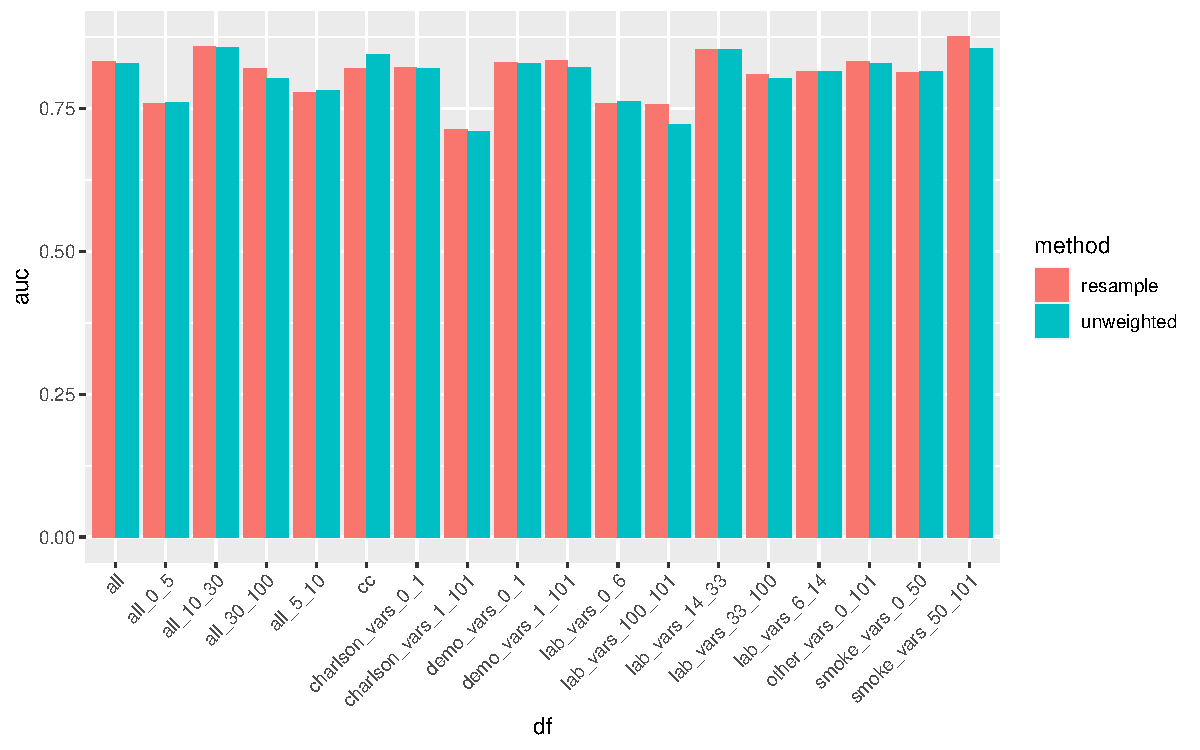
\includegraphics[width=\textwidth]{aucs.pdf}
\end{center}

\newpage
\begin{center}
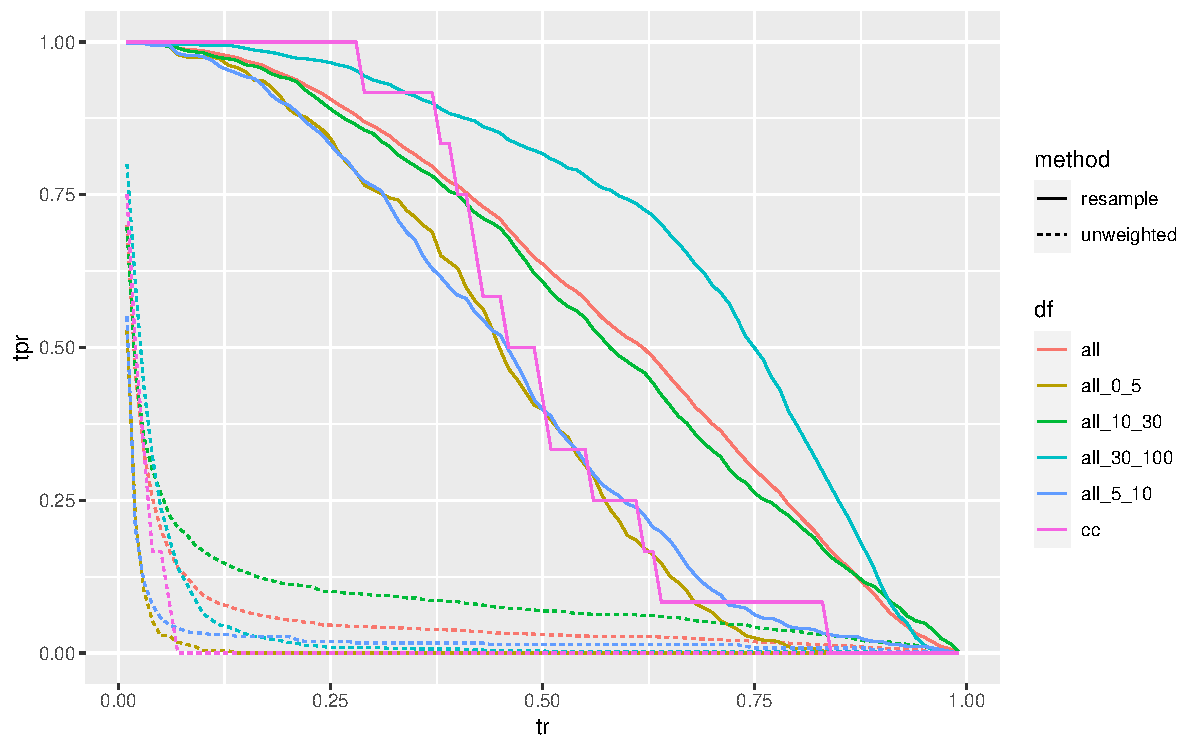
\includegraphics[width=.7\textwidth]{tpr_missing.pdf}
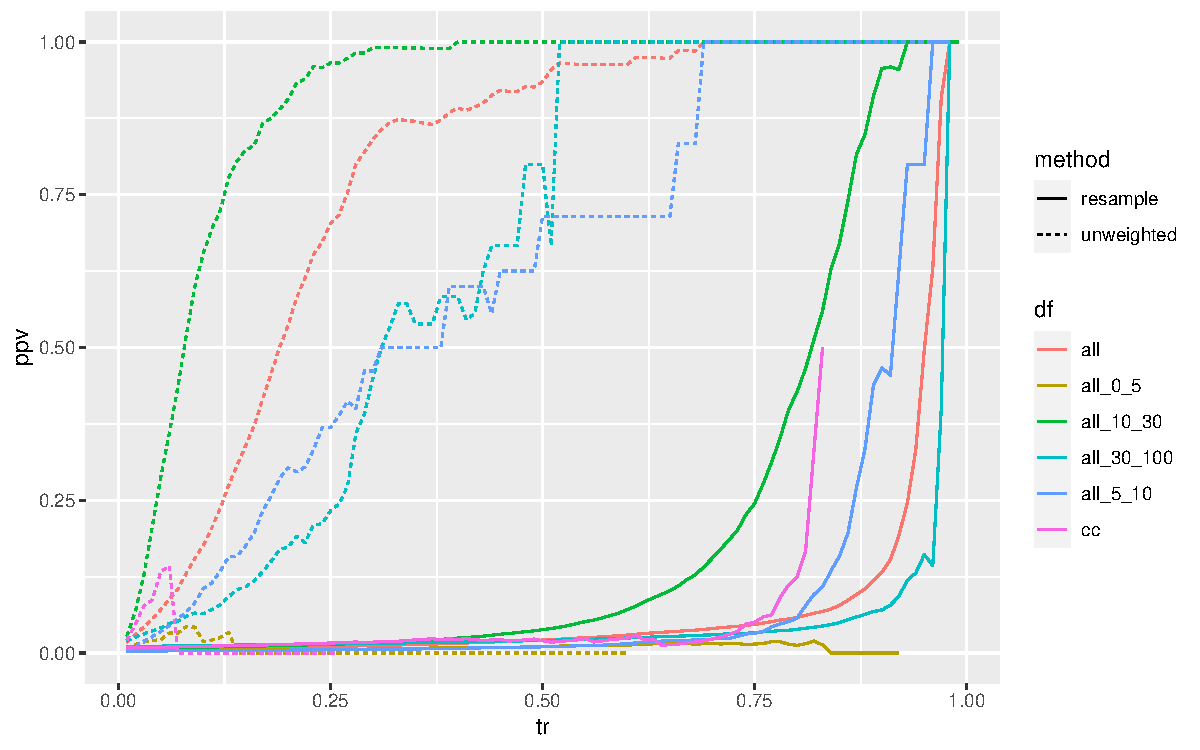
\includegraphics[width=.7\textwidth]{ppv_missing.pdf}
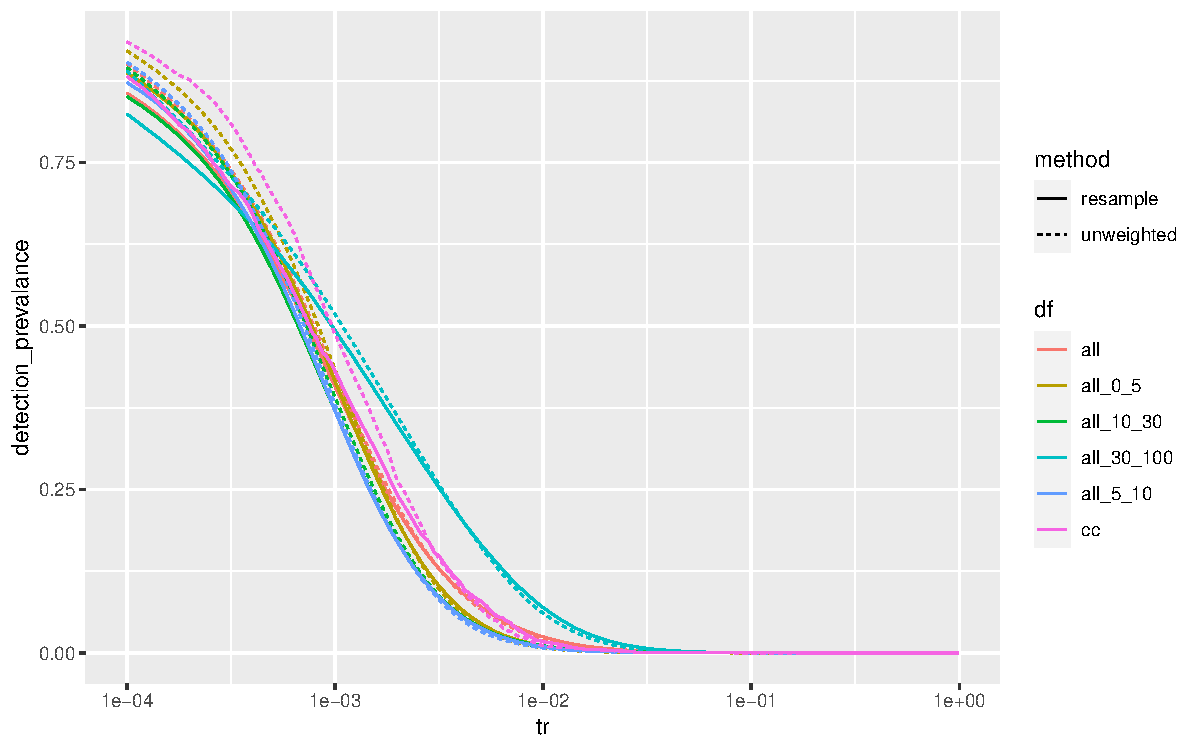
\includegraphics[width=.7\textwidth]{dp_missing.pdf}
\end{center}
\pagebreak
\begin{center}
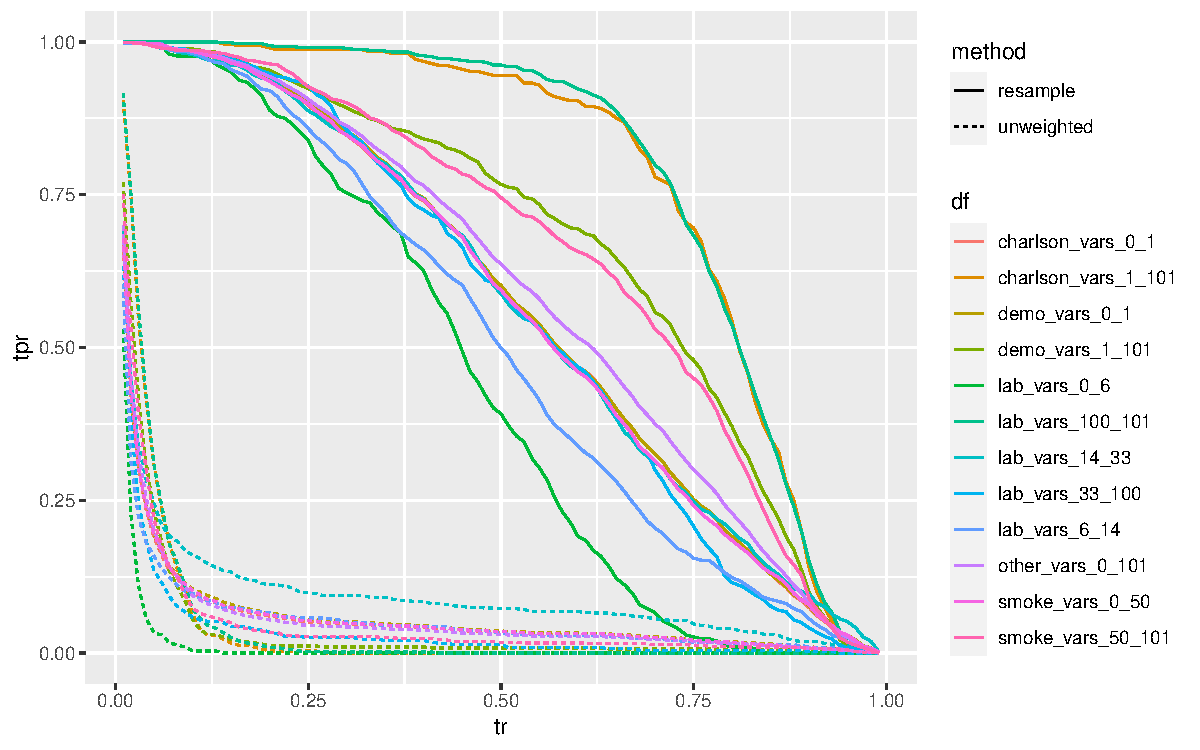
\includegraphics[width=.7\textwidth]{tpr_vars.pdf}
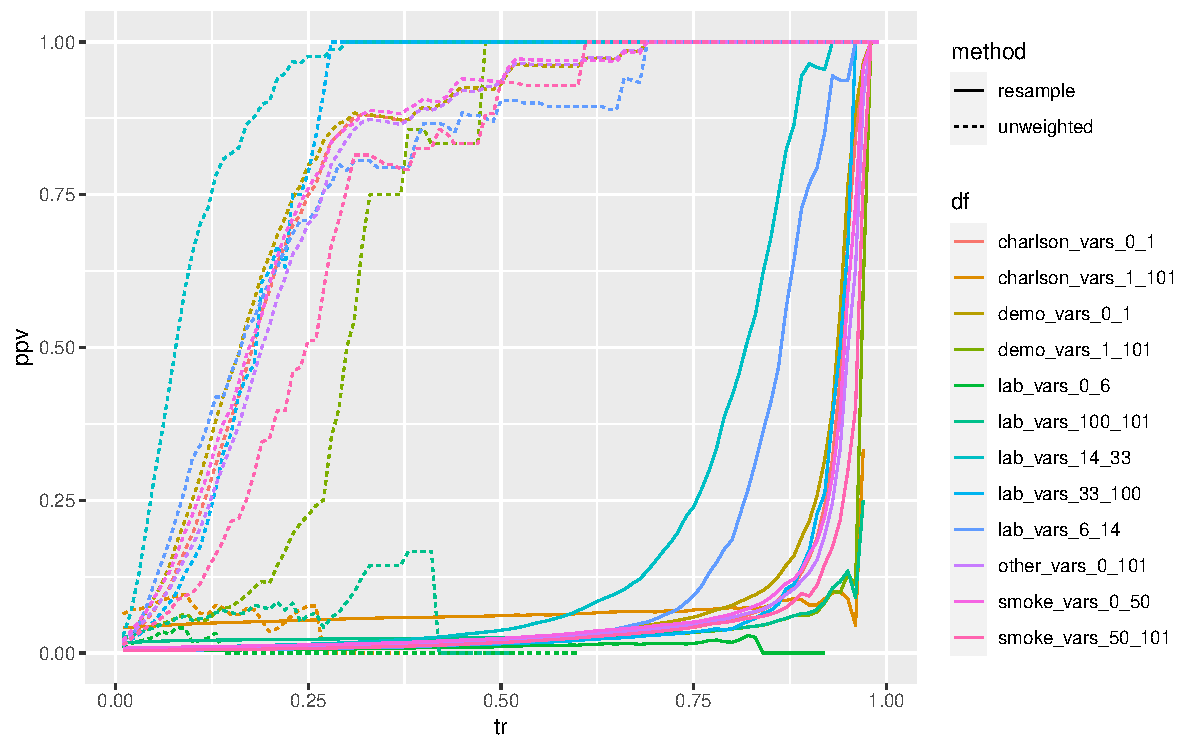
\includegraphics[width=.7\textwidth]{ppv_vars.pdf}
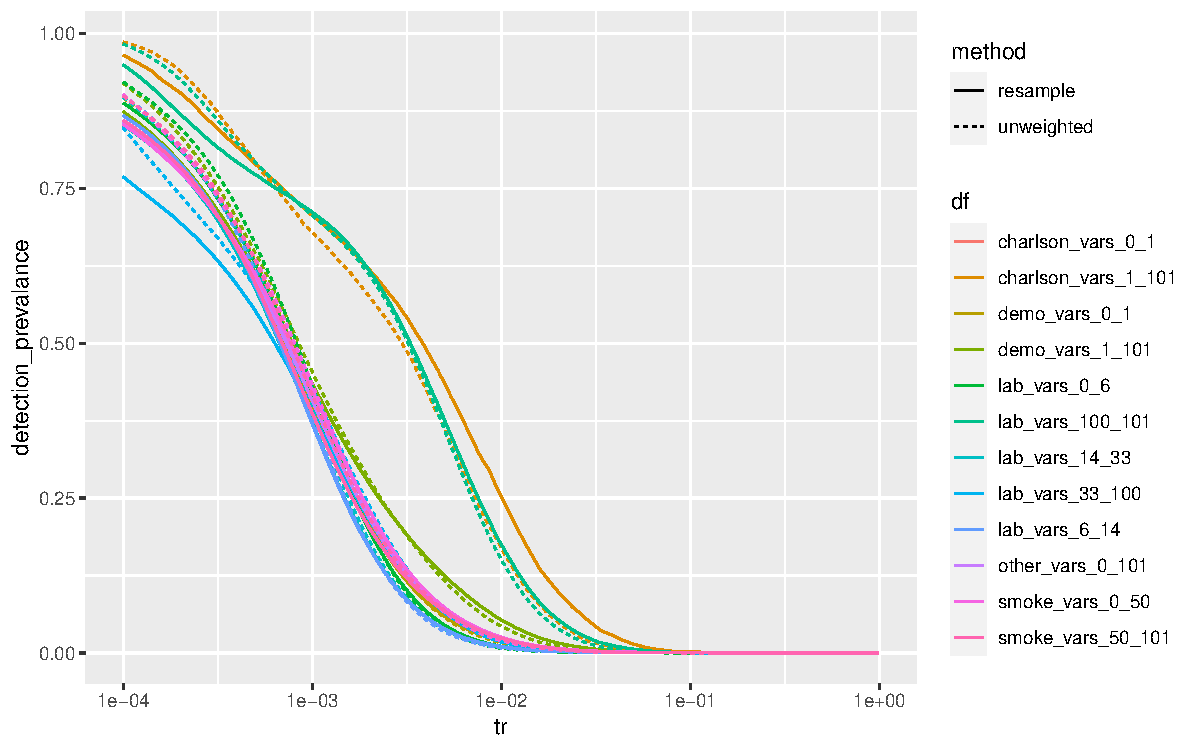
\includegraphics[width=.7\textwidth]{dp_vars.pdf}
\end{center}

\pagebreak
\begin{center}
\includegraphics[width=.45\textwidth]{roc/resample_all.pdf}
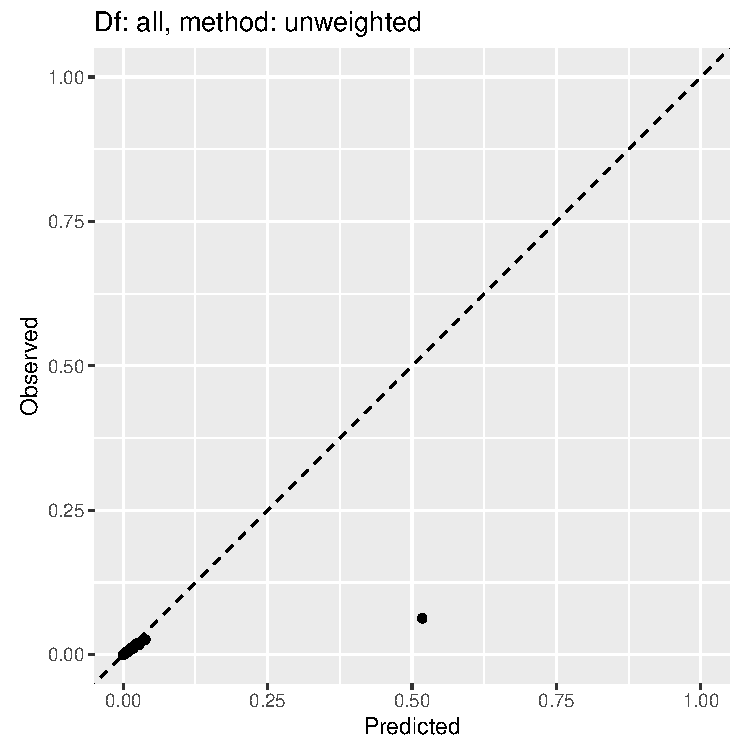
\includegraphics[width=.45\textwidth]{roc/unweighted_all.pdf}
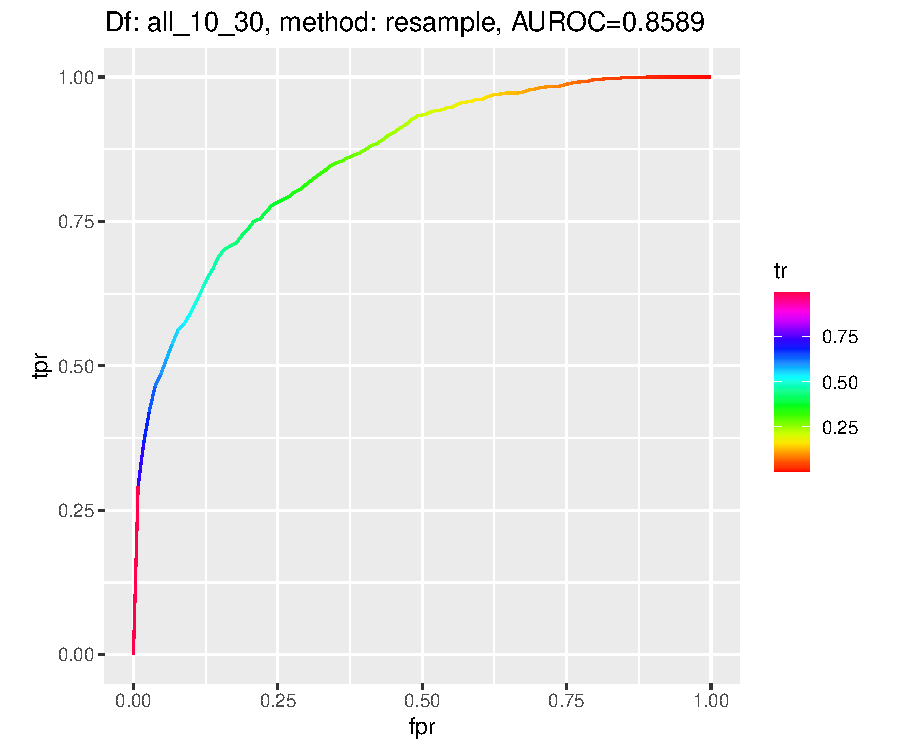
\includegraphics[width=.45\textwidth]{roc/resample_all_10_30.pdf}
\includegraphics[width=.45\textwidth]{roc/unweighted_all_10_30.pdf}
\includegraphics[width=.45\textwidth]{roc/resample_charlson_vars_1_101.pdf}
\includegraphics[width=.45\textwidth]{roc/unweighted_charlson_vars_1_101.pdf}
\end{center}


\pagebreak
\begin{center}
\includegraphics[width=.45\textwidth]{calibration_curves/resample_all.pdf}
\includegraphics[width=.45\textwidth]{calibration_curves/unweighted_all.pdf}
\includegraphics[width=.45\textwidth]{calibration_curves/resample_all_log.pdf}
\includegraphics[width=.45\textwidth]{calibration_curves/unweighted_all_log.pdf}
\end{center}


\pagebreak
\begin{center}
\includegraphics[width=.45\textwidth]{calibration_curves/resample_charlson_vars_1_101.pdf}
\includegraphics[width=.45\textwidth]{calibration_curves/unweighted_charlson_vars_1_101.pdf}
\includegraphics[width=.45\textwidth]{calibration_curves/resample_charlson_vars_1_101_log.pdf}
\includegraphics[width=.45\textwidth]{calibration_curves/unweighted_charlson_vars_1_101_log.pdf}
\end{center}



\pagebreak
\subsubsection*{11/30/2021 update}

\textbf{Recalibration}
\begin{itemize}
	\item ``resample'': upsample cases up to a balanced training set; downweight cases so they have the same total weight as the original dataset
	\begin{itemize}
		\item Example
		\item original training set: 1M controls + 5K cases
		\item after resampling: 1M controls + 1M cases
		\item reweighing: controls(1M, 1) and cases(1M, 11K/6M)
	\end{itemize}
	\item ``unweighted'': reweight cases to have the same weight as in the original dataset
	\begin{itemize}
		\item reweighing: controls(1M, 1) and cases(5K, 1M*11K/5K/6M)
	\end{itemize}
	\item Same simulations as last week but with twice as many controls
	\item Note that the fitted models are calibrated for the 11K/6M proportion
	but that is not what the testing sets are (2.5K/500K), so we expect some miscalibration on the test sets (there's a factor of $\sim 3$ between the two)
\end{itemize}

\begin{center}
\includegraphics[width=\textwidth]{2M_aucs.pdf}
\end{center}

\newpage
\begin{center}
\includegraphics[width=.7\textwidth]{2M_tpr_missing.pdf}
\includegraphics[width=.7\textwidth]{2M_ppv_missing.pdf}
\includegraphics[width=.7\textwidth]{2M_dp_missing.pdf}
\end{center}

\pagebreak
\begin{center}
\includegraphics[width=.45\textwidth]{roc/2M_resample_all.pdf}
\includegraphics[width=.45\textwidth]{roc/2M_unweighted_all.pdf}
\includegraphics[width=.45\textwidth]{roc/2M_resample_all_10_30.pdf}
\includegraphics[width=.45\textwidth]{roc/2M_unweighted_all_10_30.pdf}
\includegraphics[width=.45\textwidth]{roc/2M_resample_charlson_vars_1_101.pdf}
\includegraphics[width=.45\textwidth]{roc/2M_unweighted_charlson_vars_1_101.pdf}
\end{center}

\pagebreak
\begin{center}
\includegraphics[width=.45\textwidth]{calibration_curves/2M_resample_all.pdf}
\includegraphics[width=.45\textwidth]{calibration_curves/2M_unweighted_all.pdf}
\includegraphics[width=.45\textwidth]{calibration_curves/2M_resample_all_log.pdf}
\includegraphics[width=.45\textwidth]{calibration_curves/2M_unweighted_all_log.pdf}
\end{center}

\pagebreak
\subsubsection*{12/07/2021 update}

\paragraph*{More on calibration}

\begin{itemize}
	\item Inspection of the miscalibration observed last week showed that
	it is due to the miscalibration in the testing set. 
	\item See plot below. The dottod line has slope 6.6M/2M which is
	exactly the ratio between the testing set and the calibration
\end{itemize}

\begin{center}
\includegraphics[width=.60\textwidth]{calibration_curves/2M_resample_all_zoom.pdf}
\end{center}

\begin{itemize}
	\item Training on the whole data set is currently running: we should get correct calibration
	\item Below is the calibration table depending on the threshold
\end{itemize}

\pagebreak


\textit{Threshold in /100000, values in \%, using miscalibrated model (6.6M/2M), rule of thumb: multiply threshold by 3.2}\\
\begin{minipage}{0.5\textwidth}\small
\begin{tabular}{rccc}
\toprule
\textbf{Threshold} & \textbf{TPR} 
& \textbf{PPV} & \textbf{Det. prev.} \\
\midrule
   10 & 99.72 & 0.66 & 85.64 \\ 
     12 & 99.61 & 0.67 & 83.93 \\ 
     14 & 99.51 & 0.68 & 82.33 \\ 
     16 & 99.44 & 0.70 & 80.80 \\ 
     18 & 99.30 & 0.71 & 79.38 \\ \addlinespace
     20 & 99.19 & 0.72 & 77.98 \\ 
     22 & 99.05 & 0.73 & 76.64 \\ 
     24 & 98.84 & 0.74 & 75.31 \\ 
     26 & 98.84 & 0.76 & 73.99 \\ 
     28 & 98.60 & 0.77 & 72.76 \\ \addlinespace
     30 & 98.46 & 0.78 & 71.48 \\ 
     32 & 98.35 & 0.79 & 70.24 \\ 
     34 & 98.21 & 0.81 & 69.07 \\ 
     36 & 97.93 & 0.82 & 67.92 \\ 
     38 & 97.82 & 0.83 & 66.80 \\ \addlinespace
     40 & 97.65 & 0.84 & 65.69 \\ 
     42 & 97.44 & 0.85 & 64.60 \\ 
     44 & 97.19 & 0.87 & 63.53 \\ 
     46 & 96.98 & 0.88 & 62.50 \\ 
     48 & 96.67 & 0.89 & 61.47 \\ \addlinespace
     50 & 96.21 & 0.90 & 60.47 \\ 
     52 & 96.00 & 0.91 & 59.46 \\ 
     54 & 95.86 & 0.93 & 58.50 \\ 
     56 & 95.68 & 0.94 & 57.51 \\ 
     58 & 95.37 & 0.96 & 56.55 \\ \addlinespace
     60 & 94.91 & 0.97 & 55.62 \\ 
     62 & 94.66 & 0.98 & 54.73 \\ 
     64 & 94.38 & 0.99 & 53.85 \\ 
     66 & 94.10 & 1.01 & 52.98 \\ 
     68 & 93.86 & 1.02 & 52.12 \\ \addlinespace
     70 & 93.33 & 1.03 & 51.31 \\ 
     72 & 92.98 & 1.04 & 50.50 \\ 
     74 & 92.49 & 1.05 & 49.71 \\ 
     76 & 92.35 & 1.07 & 48.92 \\ 
     78 & 92.07 & 1.08 & 48.17 \\ 
\bottomrule
\end{tabular}

\end{minipage} \hfill
\begin{minipage}{0.5\textwidth}\small
\begin{tabular}{rccc}
\toprule
\textbf{Threshold} & \textbf{TPR} 
& \textbf{PPV} & \textbf{Det. prev.} \\
\midrule
     80 & 91.65 & 1.10 & 47.41 \\ 
     82 & 91.33 & 1.11 & 46.66 \\ 
     84 & 91.08 & 1.12 & 45.94 \\ 
     86 & 90.70 & 1.14 & 45.24 \\ 
     88 & 90.17 & 1.15 & 44.56 \\ \addlinespace
     90 & 89.93 & 1.16 & 43.90 \\ 
     92 & 89.36 & 1.17 & 43.23 \\ 
     94 & 89.08 & 1.18 & 42.61 \\ 
     96 & 88.77 & 1.20 & 41.96 \\ 
     98 & 88.31 & 1.21 & 41.34 \\ \addlinespace
    100 & 87.89 & 1.22 & 40.75 \\ 
    120 & 84.49 & 1.35 & 35.34 \\ 
    140 & 80.94 & 1.48 & 30.94 \\ 
    160 & 78.31 & 1.62 & 27.34 \\ 
    180 & 75.36 & 1.76 & 24.32 \\ \addlinespace
    200 & 71.85 & 1.87 & 21.81 \\ 
    220 & 69.71 & 2.01 & 19.68 \\ 
    240 & 67.22 & 2.13 & 17.87 \\ 
    260 & 65.39 & 2.27 & 16.29 \\ 
    280 & 63.53 & 2.41 & 14.93 \\ \addlinespace
    300 & 61.60 & 2.54 & 13.74 \\ 
    320 & 59.99 & 2.67 & 12.71 \\ 
    340 & 58.23 & 2.80 & 11.79 \\ 
    360 & 56.55 & 2.93 & 10.95 \\ 
    380 & 55.46 & 3.07 & 10.22 \\ \addlinespace
    400 & 54.12 & 3.20 & 9.57 \\ 
    420 & 52.51 & 3.32 & 8.95 \\ 
    440 & 51.07 & 3.43 & 8.43 \\ 
    460 & 49.74 & 3.54 & 7.96 \\ 
    480 & 48.51 & 3.66 & 7.51 \\ \addlinespace
    500 & 47.24 & 3.78 & 7.08 \\ 
    600 & 41.87 & 4.33 & 5.48 \\ 
    700 & 37.77 & 4.91 & 4.35 \\  
    800 & 34.40 & 5.48 & 3.56 \\ 
    900 & 31.59 & 6.07 & 2.95 \\
\bottomrule
\end{tabular}

\end{minipage}




\pagebreak
\subsubsection*{12/14/2021 update}

\begin{itemize}
	\item Follow-up on last week: 
	\begin{itemize}
		\item We were unsure why the miscalibration was in the observed direction
		\item Solution: we needed to remember that the testing sets
		contained 3x too many cases compared to the training set
		\item This explains why the observed proportion was 3x higher than expected
		\item The fitted probabilities were correct, but the case incidence in the testing set was incorrect
	\end{itemize}
	\item Results using all 6M controls are in!
	\item Essentially the same as before with slightly improved AUC (0.8459 vs 0.8439); calibration in the testing set is improved
	\item We have the same proportion on all sets (training, validation, testing) which makes the model calibrated to the correct incidence and the
	evaluation uses the correct incidence as well.
	\item Threshold selection: similar evaluation metrics except ppv/3
\end{itemize}

\pagebreak
\begin{center}
\includegraphics[width=.45\textwidth]{calibration_curves/all_resample_all.pdf}
\includegraphics[width=.45\textwidth]{calibration_curves/all_unweighted_all.pdf}
\includegraphics[width=.45\textwidth]{calibration_curves/all_resample_all_log.pdf}
\includegraphics[width=.45\textwidth]{calibration_curves/all_unweighted_all_log.pdf}
\end{center}

\newpage
\begin{center}
\includegraphics[width=.7\textwidth]{all_tpr_missing.pdf}
\includegraphics[width=.7\textwidth]{all_ppv_missing.pdf}
\includegraphics[width=.7\textwidth]{all_dp_missing.pdf}
\end{center}


\begin{minipage}{0.5\textwidth}\small
\begin{tabular}{rccc}
\toprule
\textbf{Threshold} & \textbf{TPR} 
& \textbf{PPV} & \textbf{Det. prev.} \\
\midrule
   10 & 99.79 & 0.21 & 82.47 \\ 
     12 & 99.68 & 0.21 & 80.65 \\ 
     14 & 99.51 & 0.22 & 78.94 \\ 
     16 & 99.33 & 0.22 & 77.34 \\ 
     18 & 99.23 & 0.22 & 75.82 \\  \addlinespace
     20 & 99.12 & 0.23 & 74.37 \\ 
     22 & 98.91 & 0.23 & 72.96 \\ 
     24 & 98.56 & 0.24 & 71.60 \\ 
     26 & 98.28 & 0.24 & 70.27 \\ 
     28 & 98.07 & 0.24 & 68.99 \\ \addlinespace
     30 & 97.86 & 0.25 & 67.72 \\ 
     32 & 97.61 & 0.25 & 66.51 \\ 
     34 & 97.30 & 0.26 & 65.33 \\ 
     36 & 96.91 & 0.26 & 64.16 \\ 
     38 & 96.77 & 0.26 & 63.03 \\ \addlinespace
     40 & 96.60 & 0.27 & 61.91 \\ 
     42 & 96.28 & 0.27 & 60.83 \\ 
     44 & 95.75 & 0.27 & 59.77 \\ 
     46 & 95.37 & 0.28 & 58.72 \\ 
     48 & 95.05 & 0.28 & 57.69 \\ \addlinespace
     50 & 94.49 & 0.29 & 56.70 \\ 
     52 & 94.28 & 0.29 & 55.71 \\ 
     54 & 94.03 & 0.29 & 54.76 \\ 
     56 & 93.72 & 0.30 & 53.81 \\ 
     58 & 93.37 & 0.30 & 52.91 \\ \addlinespace
     60 & 92.91 & 0.31 & 52.00 \\ 
     62 & 92.56 & 0.31 & 51.14 \\ 
     64 & 92.31 & 0.31 & 50.28 \\ 
     66 & 91.79 & 0.32 & 49.45 \\ 
     68 & 91.30 & 0.32 & 48.64 \\ \addlinespace
     70 & 91.19 & 0.33 & 47.84 \\ 
     72 & 90.91 & 0.33 & 47.06 \\ 
     74 & 90.59 & 0.34 & 46.30 \\ 
     76 & 90.14 & 0.34 & 45.56 \\ 
     78 & 89.79 & 0.34 & 44.82 \\ 
     
\bottomrule
\end{tabular}

\end{minipage} \hfill
\begin{minipage}{0.5\textwidth}\small
\begin{tabular}{rccc}
\toprule
\textbf{Threshold} & \textbf{TPR} 
& \textbf{PPV} & \textbf{Det. prev.} \\
\midrule
     80 & 89.61 & 0.35 & 44.11 \\ 
     82 & 89.26 & 0.35 & 43.41 \\ 
     84 & 88.94 & 0.36 & 42.73 \\ 
     86 & 88.49 & 0.36 & 42.06 \\ 
     88 & 88.03 & 0.36 & 41.41 \\ \addlinespace
     90 & 87.71 & 0.37 & 40.77 \\ 
     92 & 87.43 & 0.37 & 40.14 \\ 
     94 & 87.05 & 0.38 & 39.54 \\ 
     96 & 86.38 & 0.38 & 38.95 \\ 
     98 & 86.00 & 0.38 & 38.37 \\ \addlinespace
    100 & 85.68 & 0.39 & 37.80 \\ 
    120 & 82.59 & 0.43 & 32.72 \\ 
    140 & 78.98 & 0.47 & 28.58 \\ 
    160 & 76.20 & 0.52 & 25.18 \\ 
    180 & 73.82 & 0.57 & 22.37 \\  \addlinespace
	200 & 71.29 & 0.61 & 20.00 \\ 
    220 & 68.87 & 0.66 & 18.01 \\ 
    240 & 66.80 & 0.70 & 16.30 \\ 
    260 & 64.55 & 0.75 & 14.84 \\ 
    280 & 62.48 & 0.79 & 13.57 \\   \addlinespace
    300 & 60.62 & 0.83 & 12.46 \\ 
    320 & 58.97 & 0.88 & 11.50 \\ 
    340 & 57.04 & 0.92 & 10.65 \\ 
    360 & 56.02 & 0.97 & 9.89 \\ 
    380 & 54.62 & 1.02 & 9.21 \\   \addlinespace
    400 & 53.32 & 1.06 & 8.61 \\ 
    500 & 47.31 & 1.28 & 6.33 \\ 
    600 & 42.86 & 1.51 & 4.87 \\ 
    700 & 39.24 & 1.74 & 3.86 \\ 
    800 & 36.57 & 2.00 & 3.14 \\    \addlinespace
    900 & 33.17 & 2.18 & 2.61 \\ 
   1000 & 31.27 & 2.43 & 2.20 \\ 
   2000 & 21.83 & 5.87 & 0.64 \\
   5000 & 11.51 & 21.28 & 0.09 \\ 
   10000 & 7.83 & 53.61 & 0.03 \\ 
\bottomrule
\end{tabular}

\end{minipage}


\pagebreak
\begin{center}
\includegraphics[width=.45\textwidth]{roc/all_resample_all.pdf}
\includegraphics[width=.45\textwidth]{roc/all_unweighted_all.pdf}
\includegraphics[width=.45\textwidth]{roc/all_resample_all_10_30.pdf}
\includegraphics[width=.45\textwidth]{roc/all_unweighted_all_10_30.pdf}
\includegraphics[width=.45\textwidth]{roc/all_resample_charlson_vars_1_101.pdf}
\includegraphics[width=.45\textwidth]{roc/all_unweighted_charlson_vars_1_101.pdf}
\end{center}

\pagebreak
\begin{center}
\includegraphics[width=\textwidth]{all_aucs.pdf}
\end{center}





\pagebreak
\subsubsection*{01/04/2022 update}

\paragraph*{Some follow-ups}
\begin{itemize}
	\item Patient data importance:
	\begin{itemize}
		\item Smoking status (current: 121/239, former:52/239)
		\item HIV indicator (231/239)
	\end{itemize}
	\item Calibration metrics
	\begin{itemize}
		\item resampling, using all data (50-25-25 split)
		\item Create 51 bins with equal number of observations
		\begin{itemize}
			\item i.e., every 2nd percentile
			\item i.e., the 0.00, 0.02, ..., 0.98, 1.00 quantiles
			\item n.b., the last bin is very large [0.0106, 1.0000] and causes problem to compute ``expected'' counts
		\end{itemize}
		\item Using all 51 bins:
		\begin{itemize}
			\item Pearson correlation (0.920, 95\% c.i. [0.864,0.954])
			\item Spearman correlation (0.988)
			\item Hosmer-Lemeshow (H=30593, df=49, p$<$2.2e-16)
		\end{itemize}
		\item Using all but last bin:
		\begin{itemize}
			\item Pearson correlation (0.997, 95\% c.i. [0.995, 0.998])
			\item Spearman correlation (0.988)
			\item Hosmer-Lemeshow (H=42.7, df=48, p=0.690)
		\end{itemize}
	\end{itemize}
\end{itemize}


\paragraph*{Comparison to Kunzmann}

\begin{itemize}
	\item ``Esophagal condition'': 
	\begin{itemize}
		\item I could only match GERD and H2R
		
	\end{itemize}
	\item Their cohort has much fewer smokers (US vs UK?, 40\% missing?)
	\item Estimated OR compared to theirs
	\begin{itemize}
		\item Age \& Sex seem to have similar effect
		\item BMI and smoking seem to have a weaker effect (smoking status
		has a lot of missing values, so SRS imputation should hide effect)
		\item Esophagal condition, despite the mismatch, seem to have a similar effect
	\end{itemize}
\end{itemize}




\begin{table}[h]
\begin{tabular}{llrrcc}
\toprule
\multicolumn{2}{l}{Variable} & No EAC & EAC & Kunzmann OR (CI) & OR\\
\midrule
\multicolumn{2}{l}{Age} &&&& \\
& 0-50 & 1,094,536 & 187 & -- &  0.20\\
& 50-55 & 435,106 & 400 & 1.00 (reference) & 1.00\\
& 55-60 & 563,542 & 1,097 & 1.99 (1.11--3.65) & 2.19\\
& 60-65 & 792,624 & 2,053 & 2.76 (1.60--4.74) & 2.96\\
& 65+ & 2,082,924 & 4,770 & 4.03 (2.36--6.89) & 3.18\\ \addlinespace
\multicolumn{2}{l}{Sex} &&&& \\
& Female & 346,096 & 50 & 1.00 (reference) & 1.00\\
& Male & 4,632,189 & 8496 & 5.16 (3.58--7.44) & 6.60\\ \addlinespace
\multicolumn{2}{l}{BMI} &&&& \\
& 0-25 & 1,024,990 & 1,531 & 1.00 (reference) & 1.00\\
& 25-30 & 1,753,719 & 2,640 & 1.50 (1.02--2.21) & 1.00\\
& 30-35 & 1,135,392 & 1,841 & 1.91 (1.25--2.94) & 1.16\\
& 35+ & 664,785 & 1,310 & 2.97 (1.79--4.94) & 1.57\\ \addlinespace
\multicolumn{2}{l}{Smoking} &&&& \\
& Never & 405,221 & 502 & 1.00 (reference) & 1.00\\
& Former & 2,031,897 & 3,705 & 2.03 (1.47--2.80) & 1.05\\
& Current & 2,253,878 & 4,083 & 3.83 (2.59--5.66) & 1.35\\ \addlinespace
\multicolumn{2}{l}{Esophagal condition} &&&& \\
& No & 346,096 & 50 & 1.00 (reference) & 1.00\\
& Yes & 4,632,189 & 8496 & 1.88 (1.39--2.54) & 1.44\\
\bottomrule
\end{tabular}
\end{table}


\paragraph*{Sensitivity analyses}

\begin{itemize}
	\item 2--5: 
	\begin{itemize}
		\item 4 years of data, predicting 1 years ahead
		\item usual analysis
	\end{itemize}
	\item 4--5: 
	\begin{itemize}
		\item 2 years of data, predicting 3 years ahead
		\item i.e., using year -5 and -4 to predict outcome
	\end{itemize}
	\item same pipeline as before, using 100K controls
	\item AUCs: 0.7837 (2--5) vs 0.7565 (4--5)
	\item Models are miscalibrated, needs to be improved ... 
\end{itemize}




\paragraph*{Other updates}

\begin{itemize}
	\item Currently working on wrapping everything in a R package
	for simpler/easier usage and deployment.
	\item Also, implementation of some functions making sensitivity analyses easier (i.e., automating the data preprocessing)
	\item Starts with the assumptions that the user would input the same file
	as we got (patient info, medication, codes, labs)
\end{itemize}




\pagebreak
\subsubsection*{01/04/2022 update follow-up}

\paragraph*{Sample sizes}
\begin{itemize}
	\item Training set (75\%): 4,986,831 observations, 8,546 cases, 4,978,285 controls
	\begin{itemize}
		\item Further split in training + validation
		\item Training set (50\%): 3,324,554 observations, 5,697 cases 3,318,857 controls
		\item Validation set (25\%): 1,662,277 observations, 2,849 cases 1,659,428 controls
	\end{itemize}
	\item Testing set (25\%): 1,662,277 observations, 2,849 cases, 1,659,428 controls
\end{itemize}


\paragraph*{HUNT method}
\begin{itemize}
	\item This is not a logistic regression model so there is not
	really an ``intercept'' per se, only a baseline hazard when
	all variables are turned off. The baseline hazard seems to be 3.6.
	\item In any case, this does not really matter for computing
	AUC and plotting the ROC curve as we would only multiply all
	rates by some factor and this would produce the same results
	\item I will not be providing classification metrics 
	(sensitivity, specificity, etc.) as this would require choosing 
	a threshold. Let me know if you'd like to have them anyway.
\end{itemize}


\paragraph*{Comparison to HUNT and Kunzmann}
\begin{itemize}
	\item Take the original testing set (25\%: 2,849 cases, 1.66M controls)
	\item Subset to observations that are complete for both HUNT and Kunzmann 
	(i.e., with observed age, sex, bmi, smoking status, GERD, H2R, PPI)
	\item Bin variables in the same way as original papers; construct the same indicators (smoking and esophagal condition)
	\item Resulting test set: 1,816 cases, 872,093 controls
	\item Used to compute a score using all three methods (xgboost, HUNT, Kunzmann)
	\item Plot ROC curves, and compute AUC
	\begin{itemize}
		\item xgboost: 0.7869407
		\item HUNT: 0.6500223
		\item Kunzmann: 0.7046042
	\end{itemize}
\end{itemize}
\begin{center}
\includegraphics[width=\textwidth]{xgb_kunzmann_hunt_roc.pdf}
\end{center}

\newpage


\paragraph*{Window comparison}
\begin{itemize}
	\item Years 2--5 vs 4--5 to predict outcome
	\item Same patients in both test sets (same test set as previously: 2.8K cases, 1.66M controls)
	\item Model: trained on 2--5 data
	\item AUCs:
	\begin{itemize}
		\item 2--5: 0.8468027
		\item 4--5: 0.7950466
	\end{itemize}
\end{itemize}
\begin{center}
\includegraphics[width=\textwidth]{window_roc.pdf}
\end{center}





\pagebreak
\subsubsection*{01/11/2022 update}

\begin{itemize}
	\item Server maintenance over the last few days ... 
	\item Sensitivity analyses:
		\begin{itemize}
			\item Data preparation for any prediction window (fewer years, later prediction, etc.)
			\begin{itemize}
				\item e.g. 5-1 to predict 0, 5-4 to predict 0, 2-1 to predict 0, etc.
				\item The R package will allow to construct these dataset very easily (just change parameters)
			\end{itemize}
			\item EAC vs EGJAC: 
			\begin{itemize}
			\item how to get this information? (ICD 10: C15.x vs C15.5?; ICD9: 150.x vs 150.2/5?) 
			\item We were always working with `CaseControl' which was precomputed
			\item Goal: Compare whether separate models does better than a single model? 
			\item Compare to HUNT \& Kunzmann to check if this explain the big discrepancy?
			\end{itemize}
		\end{itemize}
	\item Implementation:
		\begin{itemize}
			\item Working on an R package (hosted on GitLab)
			\item Input: SAS files structured as before containing info for a set of patients
			\item Read SAS Files, construct standardized data frame, 
			use xgboost model to obtain predictions (averaged over multiple SRS for missing values)
			\item Output: (ID, risk score). Format? 
			\item Standard R package documentation
		\end{itemize}
\end{itemize}



\pagebreak
\subsubsection*{01/18/2022 update}

Added screening guidelines to ROC plot (see below)
\begin{itemize}
		\item Kunzmann uses more BMI and age bins than HUNT
		\item Kunzmann uses medication data in addition to GERD
		\item The guidelines uses even less information and simpler combination 
		\item NB: we cannot have the exact Kunzmann given our data, especially the `esophagal condition' indicator is incomplete
		\item NB: similarly for guidelines, we are missing family history and other clinical information
\end{itemize}

\begin{center}
\includegraphics[width=\textwidth]{xgb_kunzmann_hunt_roc.pdf}
\end{center}

\clearpage

Other updates
\begin{itemize}
	\item Waiting on EAC/EGJAC indicators
	\item R package:
	\begin{itemize}
		\item Data processing functions complete
		\item Next: use model to obtain scores and ouput
	\end{itemize}
	\item Prediction window sensitivity analyses:
	\begin{itemize}
		\item Takes a long time to preprocess the data
		\item Ran into a small bug, could not finish processing
		\item Once processing is done, easy to get performance
	\end{itemize}
\end{itemize}




\pagebreak
\subsubsection*{01/25/2022 update}

\textbf{Last week follow-up}
\begin{itemize}
	\item There was a slight logical error in my calculation of the screening guideline
	\item Still essentially the same results, except two are pushed to top right
	\item Any guidline requiring GERD is capped
	\begin{itemize}
		\item Prevalance is around 34\% in cases
		\item This means Sensitivity can be at most 34\% for those guidelines
		\item Prevalance around 27\% in controls; other risk factors reduce the FPR a bit
	\end{itemize}
\end{itemize}


\begin{center}
\includegraphics[width=\textwidth]{xgb_kunzmann_hunt_screening_roc.pdf}
\end{center}

\begin{table}
\centering
\begin{tabular}{crrrr}
\toprule 
 & \multicolumn{2}{c}{Controls} & \multicolumn{2}{c}{Cases}\tabularnewline
\cmidrule(lr){2-3}\cmidrule(l){4-5} 
Nb. of risk factors & N & \% & N & \%\tabularnewline
\midrule
0 & 1,853 & 0.2 & 0 & 0.0\tabularnewline
1 & 9,410 & 1.2 & 1 & 0.1\tabularnewline
2 & 44,871 & 5.6 & 4 & 0.2\tabularnewline
3 & 160,169 & 20.1 & 110 & 6.5\tabularnewline
4 & 313,723 & 39.5 & 635 & 37.6\tabularnewline
5 & 217,734 & 27.4 & 731 & 43.3\tabularnewline
6 & 47,169 & 5.9 & 207 & 12.3\tabularnewline
\cmidrule(lr){2-3}\cmidrule(l){4-5} 
 & 794,911 & 100.0 & 1,688 & 100.0\tabularnewline
\bottomrule
\end{tabular}
\end{table}

\clearpage\newpage

\textbf{Sensitivity analysis on prediction window}
\begin{itemize}
	\item I finally have the results!
	\item Predicting from farther away (+ decreasing aggregation window)
	\begin{itemize}
		\item Removing the latest year has essentially no effect
		\item Removing the last two years or more has a noticable effect
	\end{itemize}
	\item Decreasing aggregation window (still predicting 1 year later)
	\begin{itemize}
		\item Dropping the first year has almost no effect on performance
		\item Having only 1 year leads to a large gap
	\end{itemize}
\end{itemize}

\begin{center}
\includegraphics[width=\textwidth]{sensitivity_window/roc_curves_5-x.pdf}
\end{center}



\begin{center}
\includegraphics[width=\textwidth]{sensitivity_window/roc_curves_x-1.pdf}
\end{center}



%\begin{verbatim}
%
%--------------------------------------------------------------
%CaseControl 
%       n  missing distinct     Info      Sum     Mean      Gmd 
%  796599        0        2    0.006     1688 0.002119 0.004229 
%
%--------------------------------------------------------------
%smoke_current 
%       n  missing distinct     Info      Sum     Mean      Gmd 
%  796599        0        2    0.744   361422   0.4537   0.4957 
%
%--------------------------------------------------------------
%smoke_former 
%       n  missing distinct     Info      Sum     Mean      Gmd 
%  796599        0        2    0.722   321496   0.4036   0.4814 
%
%--------------------------------------------------------------
%Gender 
%       n  missing distinct     Info      Sum     Mean      Gmd 
%  796599        0        2    0.175   747167   0.9379   0.1164 
%
%--------------------------------------------------------------
%GerdAtIndex 
%       n  missing distinct     Info      Sum     Mean      Gmd 
%  796599        0        2    0.596   217718   0.2733   0.3972 
%
%--------------------------------------------------------------
%White 
%       n  missing distinct 
%  796599        0        2 
%                        
%Value       FALSE   TRUE
%Frequency  164661 631938
%Proportion  0.207  0.793
%--------------------------------------------------------------
%smoke_ever 
%       n  missing distinct 
%  796599        0        2 
%                        
%Value       FALSE   TRUE
%Frequency  113681 682918
%Proportion  0.143  0.857
%--------------------------------------------------------------
%k_age_bin 
%       n  missing distinct 
%  796599        0        5 
%
%lowest : (50,55]  (0,50]   (55,60]  (60,65]  (65,100]
%                                                       
%Value       (50,55]   (0,50]  (55,60]  (60,65] (65,100]
%Frequency     83366   183077   108154   138410   283592
%Proportion    0.105    0.230    0.136    0.174    0.356
%--------------------------------------------------------------
%k_bmi_bin 
%       n  missing distinct 
%  796599        0        4 
%                                              
%Value        (0,25]  (25,30]  (30,35] (35,100]
%Frequency    192481   296917   193545   113656
%Proportion    0.242    0.373    0.243    0.143
%--------------------------------------------------------------
%h_age_bin 
%       n  missing distinct 
%  796599        0        4 
%                                              
%Value        (0,50]  (50,60]  (60,70] (70,100]
%Frequency    183077   191520   251849   170153
%Proportion    0.230    0.240    0.316    0.214
%--------------------------------------------------------------
%h_bmi_bin 
%       n  missing distinct 
%  796599        0        2 
%                            
%Value        (0,30] (30,100]
%Frequency    489398   307201
%Proportion    0.614    0.386
%--------------------------------------------------------------
%h_smoke_any 
%       n  missing distinct     Info      Sum     Mean      Gmd 
%  796599        0        2    0.367   682918   0.8573   0.2447 
%
%--------------------------------------------------------------
%k_ec 
%       n  missing distinct 
%  796599        0        2 
%                        
%Value       FALSE   TRUE
%Frequency  460283 336316
%Proportion  0.578  0.422
%--------------------------------------------------------------
%  CaseControl n_risk_factors  `n()`
%         <dbl>          <dbl>  <int>
% 1           0              0   1835
% 2           0              1   9410
% 3           0              2  44871
% 4           0              3 160169
% 5           0              4 313723
% 6           0              5 217734
% 7           0              6  47169
% 8           1              1      1
% 9           1              2      4
%10           1              3    110
%11           1              4    635
%12           1              5    731
%13           1              6    207
%--------------------------------------------------------------
%Proportion of "positives" by group
%  CaseControl ACG2016 ACG2022 ACP2012 AGA2011 AGA_CPU2022 ASGE2019 BSG2013 ESGE2017
%1           0  195388  202881  156560  758533      738795   216497  169244   208830
%1           0   0.246   0.255   0.197   0.954       0.929    0.272   0.213    0.263
%
%2           1     565     571     535    1686        1683      575     551      575
%2           1   0.335   0.338   0.317   0.999       0.997    0.341   0.326    0.341
%--------------------------------------------------------------
%           CaseControl
%GerdAtIndex      0      1
%          0 577768   1113
%          1 217143    575
%--------------------------------------------------------------
%\end{verbatim}

\textbf{Next steps}
\begin{itemize}
	\item EAC v EGJAC
	\item Finalizing R package
	\item Study multiple imputations (effect on performance, variance of predicted
	risk by \% of missing values and which values are missing)
\end{itemize}





\pagebreak
\subsubsection*{02/01/2022 update}

\textbf{Follow-up on last week}
\begin{itemize}
	\item Fairer comparison when predicting farther in the future
	\item Prediction window of length 2, slides over the 5y period
	\item All observations have similar amount of data, but prediction
	is farther and farther back in time (1, 2, 3 years prior)
	\item No difference between years 1 and 2, but a significant drop at the 3rd year
	\item Similar conclusion as last week
\end{itemize}



\begin{center}
\includegraphics[width=\textwidth]{sensitivity_window/roc_curves_2.pdf}
\end{center}


\newpage
\textbf{Performance on identity-defined test subsets}
\begin{itemize}
	\item Same test set as before (1.5M Controls, 3K cases)
	\item Gender: 
	\begin{itemize}
		\item 93\% Male, 7\% Female
		\item Female: 26/115K cases/control
	\end{itemize}
\end{itemize}

\begin{center}
\includegraphics[width=\textwidth]{sensitivity_identity/roc_curves_Gender.pdf}
\end{center}

\newpage
\begin{itemize}
	\item Race: 
	\begin{itemize}
		\item 80\% White, 1\% Asian, 17\% Black, 1\% Hawaiian/Pacific, 1\% Indian/Alaskan
	\end{itemize}
\end{itemize}

\begin{center}
\includegraphics[width=\textwidth]{sensitivity_identity/roc_curves_Race.pdf}
\end{center}


\newpage
\textbf{Sensitivity analysis: missing values}
\begin{itemize}
	\item For each observation:
	\begin{itemize}
		\item Get 100 imputations
		\item Get predicted risk for each imputation
		\item Compute signal-to-noise ratio over the 100 risks
	\end{itemize}
	\item High SNR means that the predicted risk does not change much 
	with imputed values; small SNR means high dependence on the imputed values
	\item Partition the test set by the number of missing values
	\item Subsets defined by whether each demographic variable is missing
\end{itemize}


\begin{center}
\includegraphics[width=\textwidth]{sensitivity_missing/nb_missing_values.pdf}
\end{center}

\begin{center}
\includegraphics[width=\textwidth]{sensitivity_missing/demo_missing_values.pdf}
\end{center}

\newpage
\textbf{Sensitivity analysis: ICD10}
\begin{itemize}
	\item Data processed, results to come
	\item I settled on using 17229 as the last end date (then use
	-3 to -1 year)
\end{itemize}

\begin{center}
\includegraphics[width=\textwidth]{sensitivity_icd10/histogram.pdf}
\end{center}

\textbf{Sensitivity analysis: Cancer type}
\begin{itemize}
	\item Trained separate models, comparison to come
\end{itemize}




\pagebreak
\subsubsection*{02/08/2022 update}


\paragraph*{ICD 9/10}
\begin{itemize}
	\item Updated histogram on previous page, now shows cases/controls
	\item It appears I have 9 years of controls, but 14 years of cases
	\item Implies no ICD controls
\end{itemize}



\paragraph*{Sensitivity analysis: Cancer type}
\begin{itemize}
	\item 3 outcomes: ANY, EAC, EGJAC (what is $y$ in the test set)
	\item 3 models: ANY, EAC, EGJAC (what is $y$ in the training set)
	\item Evaluate test performance of all three models on all three
	 outcomes (same $X$, different $y$, same patients)
	\item As expected, model x performs best on outcome x
	\item EGJAC seems much easier to predict than EAC, even though 
	there are fewer of them
	\item The ANY model is almost as good as individual models on each of
	EAC or EGJAC
	\item EGJAC is particularly worse at predicting ANY/EAC
\end{itemize}


\begin{table}[ht]
\centering
\begin{tabular}{rrrr}
  \toprule
  \multicolumn{4}{l}{\textbf{Test AUC}}\\
  & \multicolumn{3}{c}{Outcome}\\ \cmidrule(l){2-4}
Model & ANY & EAC & EGJAC \\ 
  \midrule
ANY & 0.848 & 0.806 & 0.960 \\ 
  EAC & 0.819 & 0.824 & 0.805 \\ 
  EGJAC & 0.775 & 0.698 & 0.986 \\ 
  \midrule
  \multicolumn{4}{l}{\textbf{Nb. of cases}}\\\addlinespace
  Whole sample & 11395 & 8430 & 2965 \\
  Test set & 2849 & 2087 & 762 \\
   \bottomrule
\end{tabular}
\end{table}

\begin{center}
\includegraphics[width=\textwidth]{sensitivity_cancertype/roc_curves_outcome_model.pdf}
\end{center}



\pagebreak
\subsubsection*{02/15/2022 update}

Cancer type analysis: follow-up
\begin{itemize}
	\item Subset to ``complete cases'' (wrt HUNT/Kunzmann), about 50\%
	of the original data
	\item Essentially the same results
	\item HUNT and Kunzmann: similar performance across all three outcomes
\end{itemize}


\begin{table}[ht]
\centering
\begin{tabular}{rrrr}
  \toprule
  \multicolumn{4}{l}{\textbf{Test AUC}}\\
  & \multicolumn{3}{c}{Outcome}\\ \cmidrule(l){2-4}
Model & ANY & EAC & EGJAC \\ 
  \midrule
HUNT & 0.649 & 0.650 & 0.646 \\ 
  Kunzmann & 0.708 & 0.707 & 0.712 \\ 
  \addlinespace
  ANY & 0.841 & 0.791 & 0.971 \\ 
  EAC & 0.799 & 0.802 & 0.792 \\ 
  EGJAC & 0.758 & 0.675 & 0.994 \\ 
  \midrule
  \multicolumn{4}{l}{\textbf{Nb. of cases}}\\\addlinespace
  Whole sample & 6687 & 4910 & 1777 \\
  Test set & 1688 & 1218 &  470 \\ 
   \bottomrule
\end{tabular}
\end{table}

\begin{center}
\includegraphics[width=\textwidth]{sensitivity_cancertype/roc_curves_ANY_model.pdf}
\end{center}
\begin{center}
\includegraphics[width=\textwidth]{sensitivity_cancertype/roc_curves_EAC_model.pdf}
\end{center}
\begin{center}
\includegraphics[width=\textwidth]{sensitivity_cancertype/roc_curves_EGJAC_model.pdf}
\end{center}





\pagebreak
\subsubsection*{03/01/2022 update}


\subsubsection*{New data}
\begin{itemize}
	\item I was able to process it and fit the full model over the weekend
	\item As well as some submodels for sensitivity analyses
	\item I identified a few issues, however:
	\begin{itemize}
		\item There are more cases than before (about 2x), I was expecting only
		new controls? 
		\item There were \textbf{repeated IDs} which I missed before running 
		everything (1:10,254,489, 2:27,378, 3:300, 4:16)
		\item It seems it occurs for most/all cases
		(10,287,428 + 22,781, after dropping repeated: 10,254,474 + 22,781, diff: 32954 + 0)
		\item Re-running processing at the moment
		\item Whe trying to compute Kunzmann \& HUNT, I found that Gerd was missing 
		for all cases and only for about 50\% of controls
		\item This wasn't the case before ...
	\end{itemize}
\end{itemize}


\subsubsection*{Analyses}
\begin{itemize}
	\item [ready] Calibration, ROC, AUC
	\item [ready] Threshold table
	\item [ready] Variable importance (aggregated by group/category)
	\item [ready] Partial dependence of Demographic, Comorbidities and most important features
	\item [ready] Aggregation window comparison (x-1, sliding window of size 2)
	\item [ready] Cancer type analysis
	\item [ready] Identity (Gender, Race)
	\item [to do] Comparison to Kunzmann, HUNT and guidelines
	\item [to do] ICD 10 considerations
	\item [to do] Effect of missing values, multiple imputation
	\item [to do] Others?
\end{itemize}





\begin{minipage}{0.5\textwidth}\small
\begin{tabular}{rccc}
\toprule
\textbf{Threshold} & \textbf{TPR} 
& \textbf{PPV} & \textbf{Det. prev.} \\
\midrule
 10 & 99.81 & 0.51 & 74.92 \\ 
   20 & 99.36 & 0.61 & 63.30 \\ 
   30 & 98.76 & 0.69 & 55.49 \\ 
   40 & 98.20 & 0.77 & 49.49 \\ 
   50 & 97.69 & 0.85 & 44.58 \\ \addlinespace
   55 & 97.45 & 0.89 & 42.44 \\ 
   60 & 97.13 & 0.93 & 40.50 \\ 
   65 & 96.75 & 0.97 & 38.69 \\ 
   70 & 96.44 & 1.01 & 37.02 \\ 
   75 & 96.08 & 1.05 & 35.45 \\  \addlinespace
   80 & 95.76 & 1.09 & 33.99 \\ 
   85 & 95.42 & 1.13 & 32.65 \\ 
   90 & 95.02 & 1.17 & 31.38 \\ 
   95 & 94.62 & 1.21 & 30.19 \\ 
  100 & 94.38 & 1.25 & 29.09 \\  \addlinespace
  105 & 93.97 & 1.29 & 28.03 \\ 
  110 & 93.60 & 1.34 & 27.05 \\ 
  115 & 93.24 & 1.38 & 26.11 \\ 
  120 & 92.98 & 1.42 & 25.24 \\ 
  125 & 92.65 & 1.47 & 24.39 \\  \addlinespace
  130 & 92.29 & 1.51 & 23.60 \\ 
  135 & 92.03 & 1.55 & 22.85 \\ 
  140 & 91.70 & 1.60 & 22.13 \\ 
  145 & 91.50 & 1.65 & 21.44 \\ 
  150 & 91.15 & 1.69 & 20.79 \\  \addlinespace
  155 & 90.83 & 1.74 & 20.18 \\ 
  160 & 90.49 & 1.78 & 19.59 \\ 
     
\bottomrule
\end{tabular}

\end{minipage} \hfill
\begin{minipage}{0.5\textwidth}\small
\begin{tabular}{rccc}
\toprule
\textbf{Threshold} & \textbf{TPR} 
& \textbf{PPV} & \textbf{Det. prev.} \\
\midrule
  165 & 90.12 & 1.83 & 19.03 \\ 
  170 & 89.85 & 1.88 & 18.49 \\ 
  175 & 89.60 & 1.92 & 17.98 \\ 
  180 & 89.35 & 1.97 & 17.48 \\ 
  185 & 89.03 & 2.02 & 17.01 \\  \addlinespace
  190 & 88.65 & 2.07 & 16.55 \\ 
  195 & 88.36 & 2.12 & 16.12 \\ 
  200 & 88.10 & 2.17 & 15.70 \\ 
  210 & 87.63 & 2.27 & 14.91 \\ 
  220 & 87.19 & 2.37 & 14.19 \\  \addlinespace
  230 & 86.68 & 2.48 & 13.51 \\ 
  240 & 86.21 & 2.58 & 12.89 \\ 
  250 & 85.62 & 2.68 & 12.31 \\ 
  260 & 85.20 & 2.79 & 11.77 \\ 
  270 & 84.79 & 2.91 & 11.25 \\  \addlinespace
  280 & 84.31 & 3.02 & 10.77 \\ 
  290 & 83.83 & 3.13 & 10.33 \\ 
  300 & 83.29 & 3.24 & 9.91 \\ 
  325 & 82.40 & 3.54 & 8.98 \\ 
  350 & 81.30 & 3.84 & 8.17 \\  \addlinespace
  375 & 80.44 & 4.15 & 7.48 \\ 
  400 & 79.76 & 4.48 & 6.87 \\ 
  425 & 79.02 & 4.81 & 6.34 \\ 
  450 & 78.44 & 5.16 & 5.87 \\ 
  475 & 77.77 & 5.51 & 5.45 \\
  500 & 77.12 & 5.86 & 5.08 \\ 
  \addlinespace\addlinespace\addlinespace  \addlinespace
\bottomrule
\end{tabular}

\end{minipage}


\begin{center}
\includegraphics[width=\textwidth]{figures/roc.pdf}
\end{center}


\begin{center}
\includegraphics[width=0.6\textwidth]{figures/calibration50_zoom.pdf}
\includegraphics[width=0.6\textwidth]{figures/calibration50_log.pdf}
\end{center}


\begin{center}
\includegraphics[width=\textwidth]{figures/vi_cat.pdf}
\end{center}
\begin{center}
\includegraphics[width=\textwidth]{figures/vi_group_Demographic_.pdf}
\end{center}
\begin{center}
\includegraphics[width=\textwidth]{figures/vi_group_Medication_.pdf}
\end{center}
\begin{center}
\includegraphics[width=\textwidth]{figures/vi_group_Clinical_.pdf}
\end{center}
\begin{center}
\includegraphics[width=\textwidth]{figures/vi_group_Comorbidities_.pdf}
\end{center}
\begin{center}
\includegraphics[width=\textwidth]{figures/vi_group_Lab_.pdf}
\end{center}


\begin{center}
\includegraphics[width=0.45\textwidth]{figures/pdp/ageatindex.pdf}
\includegraphics[width=0.45\textwidth]{figures/pdp/bmi.pdf}\\
\includegraphics[width=0.45\textwidth]{figures/pdp/gluc_mean.pdf}
\includegraphics[width=0.45\textwidth]{figures/pdp/GerdAtIndex.pdf}\\
\end{center}


\begin{center}
\includegraphics[width=\textwidth]{figures/roc_Race.pdf}
\end{center}

\begin{center}
\includegraphics[width=\textwidth]{figures/roc_Gender.pdf}
\end{center}

\clearpage

\begin{table}[ht]
\centering
\begin{tabular}{rrrr}
\toprule
  \multicolumn{4}{l}{\textbf{Test AUC}}\\
  & \multicolumn{3}{c}{Outcome}\\ \cmidrule(l){2-4}
Model & ANY & EAC & EGJAC \\ 
  \midrule
ANY & 0.930 & 0.920 & 0.945 \\ 
  EAC & 0.931 & 0.931 & 0.907 \\ 
  EGJAC & 0.927 & 0.808 & 0.958 \\ 
   \bottomrule
\end{tabular}
\end{table}
\begin{center}
\includegraphics[width=\textwidth]{figures/risk_testANY.pdf}
\end{center}

\begin{figure}
\begin{center}
\includegraphics[width=\textwidth]{figures/risk_testEAC.pdf}
\caption{Features that predict EGJAC are not well adjusted to predict EAC}
\end{center}
\end{figure}

\begin{figure}
\begin{center}
\includegraphics[width=\textwidth]{figures/risk_testEGJAC.pdf}
\caption{Features that predict EAC are not well adjusted to predict EGJAC (not as severe as the other way, though)}
\end{center}
\end{figure}


\begin{center}
\includegraphics[width=\textwidth]{figures/roc_window_5-x.pdf}
\end{center}
\begin{center}
\includegraphics[width=\textwidth]{figures/roc_window_2.pdf}
\end{center}




\pagebreak
\subsubsection*{03/17/2022 update}


\begin{figure}[h]
\centering
\includegraphics[width=\textwidth]{figures/histogram.pdf}
\caption{New data processed, everything looks good! No repeated entries;
correct number of cases.}
\end{figure}


\begin{figure}[h]
\centering
\includegraphics[width=\textwidth]{figures/comparison.pdf}
\caption{Similar performance as before, still outperforms Kunzmann, HUNT and
guidelines by a large margin.}
\end{figure}


\begin{figure}[h]
\centering
\includegraphics[width=0.6\textwidth]{figures/calibration50_log.pdf}
\includegraphics[width=0.6\textwidth]{figures/calibration50_zoom.pdf}
\caption{Calibration looks good, although it seems we might be  slightly
over-estimating risk above 100/100,000. In particular, it doesn't seem
perfect for the target range 100-200.}
\end{figure}

\clearpage
\begin{figure}[h]
\centering
\includegraphics[width=0.45\textwidth]{figures/vi_cat.pdf}
\includegraphics[width=0.45\textwidth]{figures/vi_group_Demographic_.pdf}
\includegraphics[width=0.45\textwidth]{figures/vi_group_Comorbidities_.pdf}
\includegraphics[width=0.45\textwidth]{figures/vi_group_Medication_.pdf}
\includegraphics[width=0.45\textwidth]{figures/vi_group_Clinical_.pdf}
\includegraphics[width=0.45\textwidth]{figures/vi_group_Lab_.pdf}
\end{figure}

\clearpage
\begin{figure}[h]
\centering
\includegraphics[width=0.45\textwidth]{figures/pdp/ageatindex.pdf}
\includegraphics[width=0.45\textwidth]{figures/pdp/bmi.pdf}
\includegraphics[width=0.45\textwidth]{figures/pdp/weight.pdf}
\includegraphics[width=0.45\textwidth]{figures/pdp/Black.pdf}
\caption{I spoke with Peter, and I think I know why weight/BMI seem off.}
\end{figure}

\clearpage
\begin{table}[h]
\centering
\begin{tabular}{rrrrrrr}
  \toprule
BMI & (0,20] & (20,25] & (25,30] & (30,35] & (35,40] & (40,100] \\ 
  \midrule
Control & 99.55 & 99.79 & 99.86 & 99.87 & 99.87 & 99.87 \\ 
  Case & 0.45 & 0.21 & 0.14 & 0.13 & 0.13 & 0.13 \\ 
   \bottomrule
\end{tabular}
\caption{Proportion of cases/controls stratified by BMI. Looking at earlier 
analyses by Peter (e.g., p.11), it seems we have the same issue. I discussed 
with Peter and he told me that was a result of BMI being collect at the index
date, not 1 year prior. Could we check at what time BMI was collected for the 
new data? \& same for weight. Can we also check that smoking status is 1 year
prior? I think these are the only ones that I do not compute myself that 
could change over time.}
\end{table}

\clearpage
\begin{figure}[h]
\centering
\includegraphics[width=0.45\textwidth]{figures/pdp/copd.pdf}
\includegraphics[width=0.45\textwidth]{figures/pdp/GerdAtIndex.pdf}
\includegraphics[width=0.45\textwidth]{figures/pdp/pvd.pdf}
\includegraphics[width=0.45\textwidth]{figures/pdp/diab_nc.pdf}
\end{figure}


\clearpage
\begin{figure}[h]
\centering
\includegraphics[width=0.45\textwidth]{figures/pdp/ppi_int.pdf}
\includegraphics[width=0.45\textwidth]{figures/pdp/colonoscopy_n.pdf}
\includegraphics[width=0.45\textwidth]{figures/pdp/labs_fobt_n.pdf}
\end{figure}


\clearpage
\begin{figure}[h]
\centering
\includegraphics[width=0.45\textwidth]{figures/pdp/hgb_max.pdf}
\includegraphics[width=0.45\textwidth]{figures/pdp/hct_max.pdf}
\includegraphics[width=0.45\textwidth]{figures/pdp/wbc_min.pdf}
\includegraphics[width=0.45\textwidth]{figures/pdp/mch_tv.pdf}
\end{figure}

\clearpage
\begin{table}[h]
\centering
\begin{tabular}{rrrr}
\toprule
  \multicolumn{4}{l}{\textbf{Test AUC}}\\
  & \multicolumn{3}{c}{Testing}\\ \cmidrule(l){2-4}
Training & ANY & EAC & EGJAC \\ 
  \midrule
ANY & 0.833 & 0.800 & 0.921 \\ 
  EAC & 0.811 & 0.811 & 0.816 \\ 
  EGJAC & 0.899 & 0.680 & 0.961 \\ 
   \bottomrule
\end{tabular}
\caption{Cancer type analysis: similar results as before, but, interestingly, 
it seems that training on EGJAC improves tesing on ANY? I need to check this again,
 it is suspicious. There is an issue with how the test sample is constructed,
I think I will redo this analysis.}
\end{table}


\clearpage
\begin{figure}[h]
\centering
\includegraphics[width=0.6\textwidth]{figures/roc_ANY.pdf}
\includegraphics[width=0.6\textwidth]{figures/roc_EAC.pdf}
\includegraphics[width=0.6\textwidth]{figures/roc_EGJAC.pdf}
\end{figure}


\clearpage
\begin{figure}[h]
\centering
\includegraphics[width=0.6\textwidth]{figures/risk_testANY.pdf}
\includegraphics[width=0.6\textwidth]{figures/risk_testEAC.pdf}
\includegraphics[width=0.6\textwidth]{figures/risk_testEGJAC.pdf}
\end{figure}



\clearpage
\begin{figure}[h]
\centering
\includegraphics[width=0.8\textwidth]{figures/roc_Race.pdf}
\includegraphics[width=0.8\textwidth]{figures/roc_Gender.pdf}
\caption{Similar results as before. NB: the first comparison is
not perfect since BMI/weight/age is still taken 1 year prior.}
\end{figure}


\clearpage
\begin{figure}[h]
\centering
\includegraphics[width=0.8\textwidth]{figures/roc_window_2.pdf}
\includegraphics[width=0.8\textwidth]{figures/roc_window_x-1.pdf}
\end{figure}


\clearpage
\begin{figure}[h]
\centering
\includegraphics[width=0.8\textwidth]{figures/roc_n_imputations.pdf}
\includegraphics[width=0.8\textwidth]{figures/prediction_switch_21x10.pdf}
\caption{Not much to gain with multiple imputation, it seems most of the
action is around the 200-300 threshold, so it doesn't seem to influnce
predictions that much! See, e.g., between 100 and 150, we get almost no change
in predictions.}
\end{figure}

\clearpage

\begin{table}[ht]
\centering
\caption{}
\begin{tabular}{lrrr}
  \toprule
Value & Clinical T & Clinical N & Clinical M \\ 
  \midrule
None & 10257853 & 10257841 & 10257914 \\ 
Total Non-null & 10429 & 10441 & 10368 \\ 
\addlinespace
88 & 2 & 2 & 2 \\
\addlinespace 
c0 & 18 & 4274 & 6524 \\ 
c1 & 1131 & 3554 & 3113 \\ 
c1A & 245 & 0 & 109 \\ 
c1B & 237 & 0 & 225 \\ 
c2 & 1239 & 945 & 0 \\ 
c2A & 78 & 0 & 0 \\ 
c2B & 34 & 0 & 0 \\ 
c3 & 3464 & 479 & 0 \\ 
c3A & 0 & 1 & 0 \\ 
c4 & 685 & 0 & 0 \\ 
c4A & 136 & 0 & 0 \\ 
c4B & 261 & 0 & 0 \\ 
\addlinespace
cX & 2751 & 1186 & 367 \\ 
pIS & 148 & 0 & 0 \\ 
p1 & 0 & 0 & 28 \\ 
   \bottomrule
\end{tabular}
\end{table}





\pagebreak
\subsubsection*{03/30/2022 update}

\begin{itemize}
	\item Started processing new cases
	\item A few follow-ups from last week
	\item Stages \& ICD 10
\end{itemize}


\begin{figure}[h]
\centering
\includegraphics[width=\textwidth]{figures/risk_stage.pdf}
\end{figure}


\begin{table}[ht]
\centering
\begin{tabular}{rrr}
  \hline
stage & auc & n \\ 
  \hline
all & 0.834 & 2814 \\ 
  \addlinespace
  I & 0.843 & 280 \\ 
  II & 0.837 & 212 \\ 
  III & 0.832 & 633 \\ 
  IV & 0.838 & 1023 \\ 
  \addlinespace
  I+ & 0.836 & 2196 \\ 
  II+ & 0.835 & 1916 \\ 
  III+ & 0.835 & 1704 \\ 
  IV+ & 0.838 & 1023 \\ 
   \hline
\end{tabular}
\caption{Essentially no difference between stages. Maybe stage III has lower
predicted risk and lower AUC, but not a lot.}
\end{table}



\clearpage


\begin{figure}[h]
\centering
\includegraphics[width=\textwidth]{figures/lab_corr.pdf}
\end{figure}

\begin{table}[ht]
\centering
\begin{tabular}{rllr}
  \hline
 & var1 & var2 & correlation \\ 
  \hline
  2 & mchc & mch & 0.569 \\ 
  3 & chlor & na & 0.578 \\ 
  6 & creat & bun & 0.617 \\ 
  8 & gluc & A1c & 0.707 \\ 
  10 & mcv & mch & 0.742 \\ 
  11 & alt & ast & 0.782 \\ 
  13 & hgb & rbc & 0.857 \\ 
  15 & chol & ldl & 0.875 \\ 
  18 & rbc & hct & 0.884 \\ 
  20 & hgb & hct & 0.976 \\ 
   \hline
\end{tabular}
\caption{HGB and HCT are indeed very higly correlated}
\end{table}


\clearpage


\begin{figure}[h]
\centering
\includegraphics[width=\textwidth]{figures/roc_icd10.pdf}
\caption{We are doing somewhat better on ICD10-only data!}
\end{figure}


\clearpage


\begin{figure}[h]
\centering
\includegraphics[width=0.4\textwidth]{figures/pdp/hct_max.pdf}
\includegraphics[width=0.4\textwidth]{figures/pdp/hgb_max.pdf} \\
\includegraphics[width=0.7\textwidth]{figures/pdp_hct_hgb.pdf}
\end{figure}


\clearpage
\pagebreak
\subsubsection*{04/26/2022 update}


\paragraph*{Representative sample (sex)}

\begin{table}[h]
\centering
\begin{tabular}{lrrr}
\toprule
\multicolumn{4}{l}{\textbf{Complete cases only}} \\
Sex & Cases & Controls & Total \\
\midrule
F & 4 & 41197 & 41201 \\
M & *33 & **41168 & 41201 \\
Total & 37 & 82365 & 82402 \\
 \midrule
\multicolumn{4}{l}{\textbf{Sex available, rest imputed}} \\
\midrule
F & 9 & 147178 & 147187 \\
M & *75 & **147112 & 147187 \\
Total & 84 & 294290 & 294374 \\
 \bottomrule
 \multicolumn{4}{r}{\textit{*sampled to 8.33:1 ratio}}\\
 \multicolumn{4}{r}{\textit{**sampled to 1:1 ratio}}
\end{tabular}
\end{table}

\begin{figure}[h]
\centering
\includegraphics[width=\textwidth]{figures/comparison_sex_complete.pdf}
\end{figure}

\begin{figure}[h]
\centering
\includegraphics[width=\textwidth]{figures/comparison_sex_imputed.pdf}
\end{figure}
  
  
 
\clearpage
\paragraph*{Age effect}

\begin{itemize}
	\item Proportion of cases by age, SHAP values, PDP and predicted risk per age
	\item All seem to indicate a drop after 60-65
\end{itemize}

\begin{figure}[h]
\centering
\includegraphics[width=\textwidth]{figures/cond_prop_age.pdf}
\end{figure}

\begin{figure}[h]
\centering
\includegraphics[width=\textwidth]{figures/risk_age.pdf}
\caption{25-, 50- and 75th percentiles}
\end{figure}

\begin{figure}[h]
\centering
\includegraphics[width=\textwidth]{figures/shap_age.pdf}
\end{figure}

\begin{figure}[h]
\centering
\includegraphics[width=\textwidth]{figures/pdp/ageatindex.pdf}
\end{figure}



 
\clearpage
\paragraph*{Variable importance via SHAP values}

\begin{itemize}
	\item SHAP values are an alternative way to inspect variable importance
	\item very broadly: for each observation, how much that feature changes the 
	model output (here: log-odds)
	\item Can be aggregated ($\text{mean}|\text{SHAP}|$) to global importance
	\item Additive measure so we can aggregate features into groups
	\item Gives a somewhat different ranking that standard VI (which gives 
	how much a feature changes the loss function)
\end{itemize}


\begin{figure}[h]
\centering
\includegraphics[width=\textwidth]{figures/shap_category.pdf}
\end{figure}
\begin{figure}[h]
\centering
\includegraphics[width=0.8\textwidth]{figures/shap_groups.pdf}
\end{figure}

\clearpage
\paragraph*{To do}
\begin{itemize}
	\item EAC v EGJAC: SHAP values
	\item PDP/SHAP before after dropping
	\item Smaller model?
	\item Finish R package (include model, quality control)
\end{itemize}


\clearpage
\pagebreak
\subsubsection*{05/03/2022 update}

\paragraph*{R package update}
\begin{itemize}
	\item Added EAC and EGJAC models
	\item Added some quality control checks
\end{itemize}


\clearpage
\pagebreak
\paragraph*{Birth cohort effect}
\begin{itemize}
	\item Using index date, age at index and knowing data ends at 2019,
	I am able to get birth year ($\pm 1$ year)
	\item 70-83yo is where the switch between $\leq 1935$ to $>1935$
	\item There is a significant change in case prevalance between the two cohorts
	for a fixed age
	\item prevalance seems flat beyond $\sim 60$yo
	\item PDP and predicted risk show some gap during the transition period
	\item There is a sudden drop at around 73yo in PDP and SHAP, which could
	indicate that the model is trying its best at modeling the birth cohort effect
\end{itemize}

\begin{figure}[h]
\centering
\includegraphics[width=0.8\textwidth]{figures/age_birth.pdf}
\end{figure}

\begin{figure}[h]
\centering
\includegraphics[width=0.8\textwidth]{figures/prop_cases_age_birth.pdf}
\end{figure}

\begin{figure}[h]
\centering
\includegraphics[width=0.8\textwidth]{figures/risk_age_birth.pdf}
\end{figure}
\begin{figure}[h]
\centering
\includegraphics[width=0.8\textwidth]{figures/age_pdp.pdf}
\end{figure}
\begin{figure}[h]
\centering
\includegraphics[width=0.8\textwidth]{figures/shape_age_birth.pdf}
\end{figure}

\clearpage
\pagebreak
\subsubsection*{05/10/2022 update}

\paragraph*{Birth cohort effect -- follow-up}

\begin{itemize}
	\item Fitted four models (on 1M controls):
	\begin{itemize}
		\item NONE: do nothing special, same model as before
		\item DROP: only fit on subjects after 1935
		\item IND: add the 1935 indicator
		\item NUM: use birth year as a feature directly
	\end{itemize}
	\item Compare prediction performance (Test AUC)
	\begin{itemize}
		\item Stratified by a few birth cohort
	\end{itemize}
	\item PDP and SHAP curves
	\item NUM: can check PDP and SHAP of birth year and compare
	\item Notes: 
	\begin{itemize}
		\item Since we use 1M controls, calibration and raw numbers will be off, 
		but the trends are still meaningful
	\end{itemize}
	\item Results:
	\begin{itemize}
		\item NUM produces the best predicted risks up to 1965; it is
		also the best overall (note that it improves on the current model)
		\item 1935 does not seem the best cutoff, more like a curve or at least the
		interval 1935-1955 has higher incidence than the rest
		\item Trees will find the ``best'' cutoff anyway ...
		\item Training only on $>1935$ subjects (DROP) or using the indicator (IND)
		 seems to alleviate the drop in age effect after 65yo, but not as well
		 as using birth year as feature (NUM)
	\end{itemize}
\end{itemize}


\begin{table}[ht]
\centering
\begin{tabular}{lrrrr}
  \toprule
  & \multicolumn{4}{c}{Test AUC} \\ \cmidrule(l){2-5}
Cohort & NONE & IND & NUM & DROP \\ 
  \midrule
All & 0.845 & 0.836 & \textbf{0.850} & 0.829 \\ 
  1900-1925 & 0.818 & 0.803 & \textbf{0.826} & 0.785 \\ 
  1925-1935 & 0.800 & 0.788 & \textbf{0.805} & 0.770 \\ 
  1935-1945 & 0.797 & 0.792 & \textbf{0.806} & 0.780 \\ 
  1945-1955 & 0.820 & 0.813 &\textbf{ 0.829} & 0.804 \\ 
  1955-1965 & 0.816 & 0.817 & \textbf{0.827} & 0.812 \\ 
  1965-1975 & \textbf{0.893} & 0.878 & 0.878 & 0.875 \\ 
  1975-2000 & \textbf{ 0.758} & 0.742 & 0.718 & 0.728 \\ 
   \bottomrule
\end{tabular}
\end{table}


\begin{figure}[h]
\centering
\includegraphics[width=1.0\textwidth]{figures/birthyear/age_birth.pdf}
\includegraphics[width=1.0\textwidth]{figures/birthyear/prop_cases_age_birth.pdf}
\end{figure}

\begin{figure}[h]
\centering
\includegraphics[width=1.0\textwidth]{figures/birthyear/pdp_models.pdf}
\includegraphics[width=1.0\textwidth]{figures/birthyear/shap_models.pdf}
\end{figure}


\begin{figure}[h]
\centering
\includegraphics[width=0.9\textwidth]{figures/birthyear/shap_num_age.pdf}
\includegraphics[width=0.9\textwidth]{figures/birthyear/shap_num_by.pdf}
\includegraphics[width=0.9\textwidth]{figures/birthyear/pdp_by.pdf}
\end{figure}

\begin{figure}[h]
\centering
\includegraphics[width=1.0\textwidth]{figures/birthyear/shap_num_age_by.pdf}
\includegraphics[width=1.0\textwidth]{figures/birthyear/shap_models.pdf}
\caption{Aggregating the effect of age and birth cohort in the NUM model
recovers the SHAP curves for age of the other models. Hence, we are decomposing the 
effect.}
\end{figure}



\clearpage
\pagebreak
\subsubsection*{05/17/2022 update}

\begin{itemize}
	\item Updated GERD calculation
	\item Refitted model with new GERD
	\begin{itemize}
		\item Improved Test AUC (0.85$\to$0.90)
		\item Increased contribution of GERD, stronger effect
	\end{itemize}	 
\end{itemize}

\begin{figure}[h]
\centering
\includegraphics[width=1.0\textwidth]{figures/roc.pdf}
\end{figure}

\begin{figure}[h]
\centering
\includegraphics[width=1.0\textwidth]{figures/comparison_ANY.pdf}
\end{figure}

\begin{figure}[h]
\centering
\includegraphics[width=1.0\textwidth]{figures/vi_group.pdf}
\end{figure}
\begin{figure}[h]
\centering
\includegraphics[width=1.0\textwidth]{figures/vi_group_Comorbidities_.pdf}
\end{figure}

\begin{figure}[h]
\centering
\includegraphics[width=1.0\textwidth]{figures/shap_groups.pdf}
\end{figure}

\begin{figure}[h]
\centering
\includegraphics[width=0.45\textwidth]{figures/pdp/GerdAtIndex.pdf}
\includegraphics[width=0.45\textwidth]{figures/pdp_new/gerd.pdf}
\includegraphics[width=0.45\textwidth]{figures/shap/GerdAtIndex.pdf}
\includegraphics[width=0.45\textwidth]{figures/shap_new/gerd.pdf}
\end{figure}




\clearpage
\pagebreak
\subsubsection*{05/24/2022 update}

Calibration with respect to birth cohort effect:
\begin{itemize}
	\item Stratify by age, birth year and index date	 
	\item Predicted risk seems to be somewhat high for 70-90 yo
	\item Same for 1920-1930 birth cohort \& 1960-1970
	\item Over-estimation for 2004-2008 patients, slight under-estimation for 2008-2016 patients
\end{itemize}



\begin{figure}[h]
\centering
\includegraphics[width=1.0\textwidth]{figures/birthyear/calibration_age_zoom.pdf}
\end{figure}

\begin{figure}[h]
\centering
\includegraphics[width=1.0\textwidth]{figures/birthyear/calibration_birthcohort_zoom.pdf}
\end{figure}

\begin{figure}[h]
\centering
\includegraphics[width=1.0\textwidth]{figures/birthyear/calibration_index_zoom.pdf}
\end{figure}



\clearpage
\pagebreak
\subsubsection*{05/31/2022 update}

Calibration with respect to birth cohort effect:
\begin{itemize}
	\item 10 bins to reduce noise
	\item Calibration for alternative models including birthyear (NONE v. IND, NUM, DROP)
\end{itemize}



\begin{figure}[h]
\centering
\includegraphics[width=1.0\textwidth]{figures/birthyear/calibration_birthcohort_zoom.pdf}
\end{figure}


\begin{figure}[h]
\centering
\includegraphics[width=1.0\textwidth]{figures/birthyear/calibration_age_zoom.pdf}
\end{figure}

\begin{figure}[h]
\centering
\includegraphics[width=1.0\textwidth]{figures/birthyear/calibration10_birthcohort_zoom.pdf}
\end{figure}

\begin{figure}[h]
\centering
\includegraphics[width=1.0\textwidth]{figures/birthyear/calibration10_birthcohort_log.pdf}
\end{figure}




\clearpage
\pagebreak
\subsubsection*{06/07/2022 update}


\paragraph*{Calibration and reporting cut-off} 
Summary of email exchange

\begin{itemize}
	\item It is hard to evaluate calibration for high-risk patients
	\item The ``last bin'' is hard to display because it is large (e.g., 740-100,000 when using 50 bins)
	\item Looking at even finer bins, we can see that calibration is decent even up to around 1,500/100,000, but these get very noisy, so it is unclear if calibration is correct or they just line up well just by chance
	\item I would advise not reporting any precise score above, say, 1,000/100,000 and only report, e.g.,  ``$>$1,000/100,000''.
\end{itemize}

\begin{figure}[h]
\centering
\includegraphics[width=0.49\textwidth]{figures/calibration50_bar_zoom.pdf}
\includegraphics[width=0.49\textwidth]{figures/calibration50_bar_log.pdf}
\end{figure}

\begin{figure}[h]
\centering
\includegraphics[width=0.49\textwidth]{figures/calibration1000_bar_zoom.pdf}
\includegraphics[width=0.49\textwidth]{figures/calibration1000_bar_log.pdf}
\end{figure}

\clearpage

\paragraph*{EGJAC risk scores}
Summary of email exchange
\begin{itemize}
	\item Rich used to three models to get predicted risk for the upcoming cohort
	\item Joel identified that EGJAC risk scores were much lower than ANY and EAC 
	\item I looked at how these distribution matches those in the testing set and I found very similar distributions
	\item This seems to indicate that the observed difference really comes from the model, not from difference in samples
	\item This lead me to look more into EGJAC's model and I found some serious miscalibration (also some for EAC, but way less)
	\item Similar behaviour as when there was imbalance between training prevlance and testing prevalance; I still don't have a good explanation for it yet.
	\item Splitting across case/control, we see the same shift between cases and control (about a 10x increase in risk), but EGJAC has some heavier tail, which seems to explain the better AUC for that model.
\end{itemize}

\begin{table}[ht]
\centering
\begin{tabular}{lrrrrrrrr}
\toprule
Model 	&n 		&Mean 		&SD 			&Min 	&Q1 			&Median 		&Q3 			&Max\\ \midrule
ANY 		&356 	&0.00233 	&0.00879 	&0e+00 	&0.00015 	&0.00063 	&0.00177 	&0.12063\\
EAC 		&356 	&0.00678 	&0.02677 	&1e-05 	&0.00025 	&0.00094 	&0.00274 	&0.34658\\
EGJAC 	&356 	&0.00003 	&0.00020 	&0e+00 	&0.00000 	&0.00000 	&0.00001 	&0.00352\\ \bottomrule
\end{tabular}
\end{table}

\begin{figure}[h]
\centering
\includegraphics[width=1.0\textwidth]{figures/risk_distribution.pdf}
\end{figure}

\begin{figure}[h]
\centering
\includegraphics[width=1.0\textwidth]{figures/risk_distribution_casecontrol.pdf}
\end{figure}


\begin{figure}[h]
\centering
\includegraphics[width=0.49\textwidth]{figures/EAC_calibration50_bar_log.pdf}
\includegraphics[width=0.49\textwidth]{figures/EGJAC_calibration50_bar_log.pdf}
\end{figure}


\clearpage
\paragraph*{GERD and ICD 10s}
Summary of email exchange
\begin{itemize}
	\item Rich noticed that none of the 356 patients had GERD=1, but GERD should be much more common (we had aorund 20\% in the original data)
	\item Current definition of GERD is
	\begin{itemize}
		\item ICD9: 787.1 (Heartburn) + 530.81 (Esophageal reflux, no esophagitis)
		\item ICD10: R12 (Heartburn)
		\item We excluded K21.9 since it requires an EGD?
		\item Does 530.81 require one?
	\end{itemize}
	\item All new patients will only have ICD10 data
	\item There were no R12 in the data, so it was to be expected to have no GERD=1
	\item Looking at prevalance of ICD codes, we see that 530.81 constitute most of the GERD=1 in ICD9 (60:1 ratio) so it is not surprising we have no GERD=1 by dropping K21.9
	\item What should we do about it? It will be important to insure that all patients (training, testing and in practice) have the same definition of features, which is not the case now since most training patients did use reflux to define GERD. 
\end{itemize}

\begin{figure}[h]
\centering
\includegraphics[width=1.0\textwidth]{figures/image.png}
\end{figure}

\end{document}
